\documentclass{article}
\usepackage[utf8]{inputenc}


\font\myfont=cmr12 at 25pt
%\title{\myfont Notes on Permanent Magnet Synchronous Machine (PMSM) Model %Predictive Control (MPC) and Operation Under Open Circuit Fault}
\font\hisfont=cmr12 at 15pt

\author{\hisfont Hakan Saraç}
\date{}


\usepackage{float}
\usepackage{comment}
\usepackage{natbib}
\usepackage{graphicx}
\usepackage{indentfirst}
\usepackage{siunitx}
\usepackage{svg}
\usepackage{hyperref}
\usepackage{amsmath, bm}
\usepackage{graphicx} 
\usepackage{pstool}
\usepackage{listings}
\usepackage{natbib}
\usepackage{graphicx}
\usepackage{epstopdf}
\usepackage{tikz}
\usepackage[utf8]{inputenc}
\usepackage{pgfplots} 
\usepackage{pgfgantt}
\usepackage{pdflscape}
\pgfplotsset{compat=newest} 
\pgfplotsset{plot coordinates/math parser=false}
\lstloadlanguages{Matlab}%
\lstset{ 
	language=Matlab,                		% choose the language of the code
%	basicstyle=10pt,       				% the size of the fonts that are used for the code
	numbers=left,                  			% where to put the line-numbers
	numberstyle=\footnotesize,      		% the size of the fonts that are used for the line-numbers
	stepnumber=1,                   			% the step between two line-numbers. If it's 1 each line will be numbered
	numbersep=5pt,                  		% how far the line-numbers are from the code
%	backgroundcolor=\color{white},  	% choose the background color. You must add \usepackage{color}
	showspaces=false,               		% show spaces adding particular underscores
	showstringspaces=false,         		% underline spaces within strings
	showtabs=false,                 			% show tabs within strings adding particular underscores
%	frame=single,	                			% adds a frame around the code
%	tabsize=2,                				% sets default tabsize to 2 spaces
%	captionpos=b,                   			% sets the caption-position to bottom
	breaklines=true,                			% sets automatic line breaking
	breakatwhitespace=false,        		% sets if automatic breaks should only happen at whitespace
	escapeinside={\%*}{*)}          		% if you want to add a comment within your code
}

\addtolength{\oddsidemargin}{-.875in}
\addtolength{\evensidemargin}{-.875in}
\addtolength{\textwidth}{1.75in}
\addtolength{\topmargin}{-.875in}
\addtolength{\textheight}{1.75in}


\begin{document}
\title{\line(1,0){250}\\\myfont Notes on Permanent Magnet Synchronous Machine (PMSM) Model Predictive Control (MPC) and Operation Under Open Circuit Fault\\\line(1,0){250}}
\maketitle
\newpage
\tableofcontents
\newpage


\section{Introduction}
In this handnote, I will be explaining my findings on PMSM control using MPC. At first, I will introduce the formula sets and PMSM state space model and how to implement MPC. Then, for a 3 phase PMSM I will be explaining my implementation and test results. After that, the implementation of MPC for a two-three-phase group machine will be discussed. Lastly, the two-three-phase group machine will be investigated under open circuit faults.

In the conclusions part, I have mentioned the problems I need to overcome and in the appendix the matlab function codes are provided.


\section{MPC for PMSM}
In the implementation of MPC, there are parameters we need to have in order to be able to make an prediction. For a motor drive application, mainly, we need to predict the torque output of the machine. 

To achieve the torque prediction, in an induction machine, the rotor flux parameters needs to be estimated. In a PMSM, since the rotor flux density is a constant known parameters, the estimation is not necessary. A control block diagram is provided in \citep{ExperimentalImplementationOfModelPredictiveControlForPermanentMagnetSynchronousMotor}.

\begin{figure}[H]
\centering
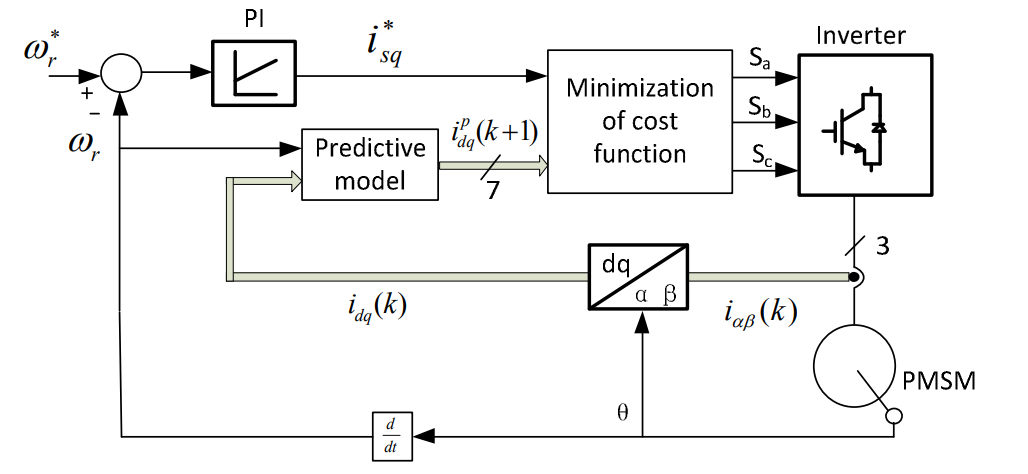
\includegraphics[scale=0.5]{Figures/MPC_PMSM_block_diagram.PNG}
\caption{MPC PMSM control block diagram \citep{ExperimentalImplementationOfModelPredictiveControlForPermanentMagnetSynchronousMotor}}
\label{fig:MpcPmsmBlockDiagram}
\end{figure}

\begin{figure}[H]
\centering
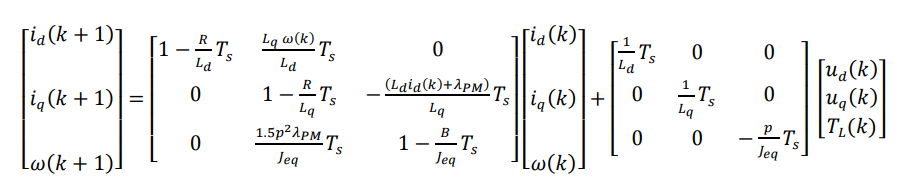
\includegraphics[scale=0.5]{Figures/StateSpaceModel.PNG}
\caption{State Space Model \citep{ExperimentalImplementationOfModelPredictiveControlForPermanentMagnetSynchronousMotor}}
\label{fig:StateSpaceModel}
\end{figure}

\section{One Module Implementation}
\subsection{Model}
The matlab model can be seen in \ref{fig:OneModuleSimulinkModel}. The matlab code inside the large function diagram is provided in Listing \ref{code:SingleModule}. Some of the properties of the simulation and machine parameters can be listed as follows:
\begin{itemize}
    \item Sampling Time = 1e-6
    \item Algorithm Frequency = 40kHz
    \item Rs = 351mOhm
    \item Ls = 3.5mHenry
    \item Back Emf At 600RPM = 80.3 Volt
    \item Flux per pole = 0.18 Weber
    \item Vdc = 270 Volts
\end{itemize}





The system operates in a stable way, however, torque ripple at steady state is considerably high.

\begin{figure}[H]
\centering
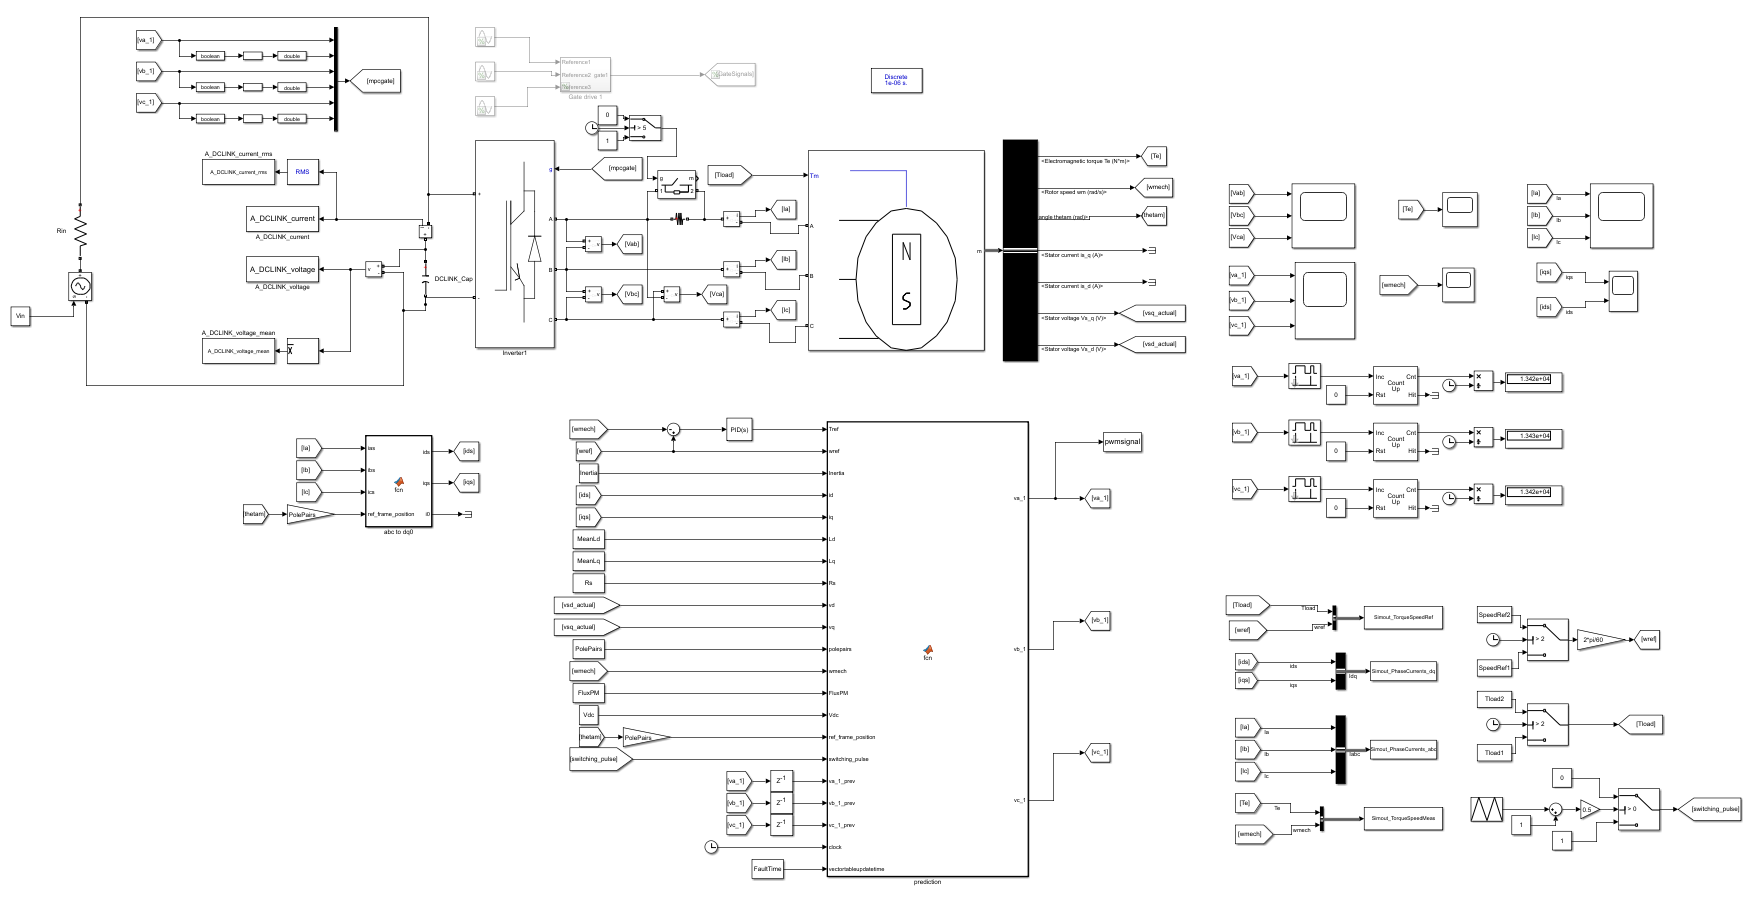
\includegraphics[scale=0.3]{Figures/OneModuleSimulinkModel.PNG}
\caption{One Module Simulink Model}
\label{fig:OneModuleSimulinkModel}
\end{figure}


\subsection{Simulation Results}

The algorithm evaluates the cost function (line \ref{line:One_Module_cost} of Listing \ref{code:SingleModule}) for 8 possible switching vectors for a two level inverter. The evalution is done for 40kHz rate. Due to the property of the MPC algorithm, the switching frequency varies. In one second, the switchings are around 12-14 kHz. For the beginning, the cost function only evaluates the torque error and the Id current. Some limits for the protection can be seen in line 41 of Listing \ref{code:SingleModule}.

The obtained results are listed in Figures \ref{fig:Tload_Wshaft_OneModule}, \ref{fig:Current_dq_OneModule}, \ref{fig:Current_abc_OneModule}.

\begin{figure}[H]
\centering
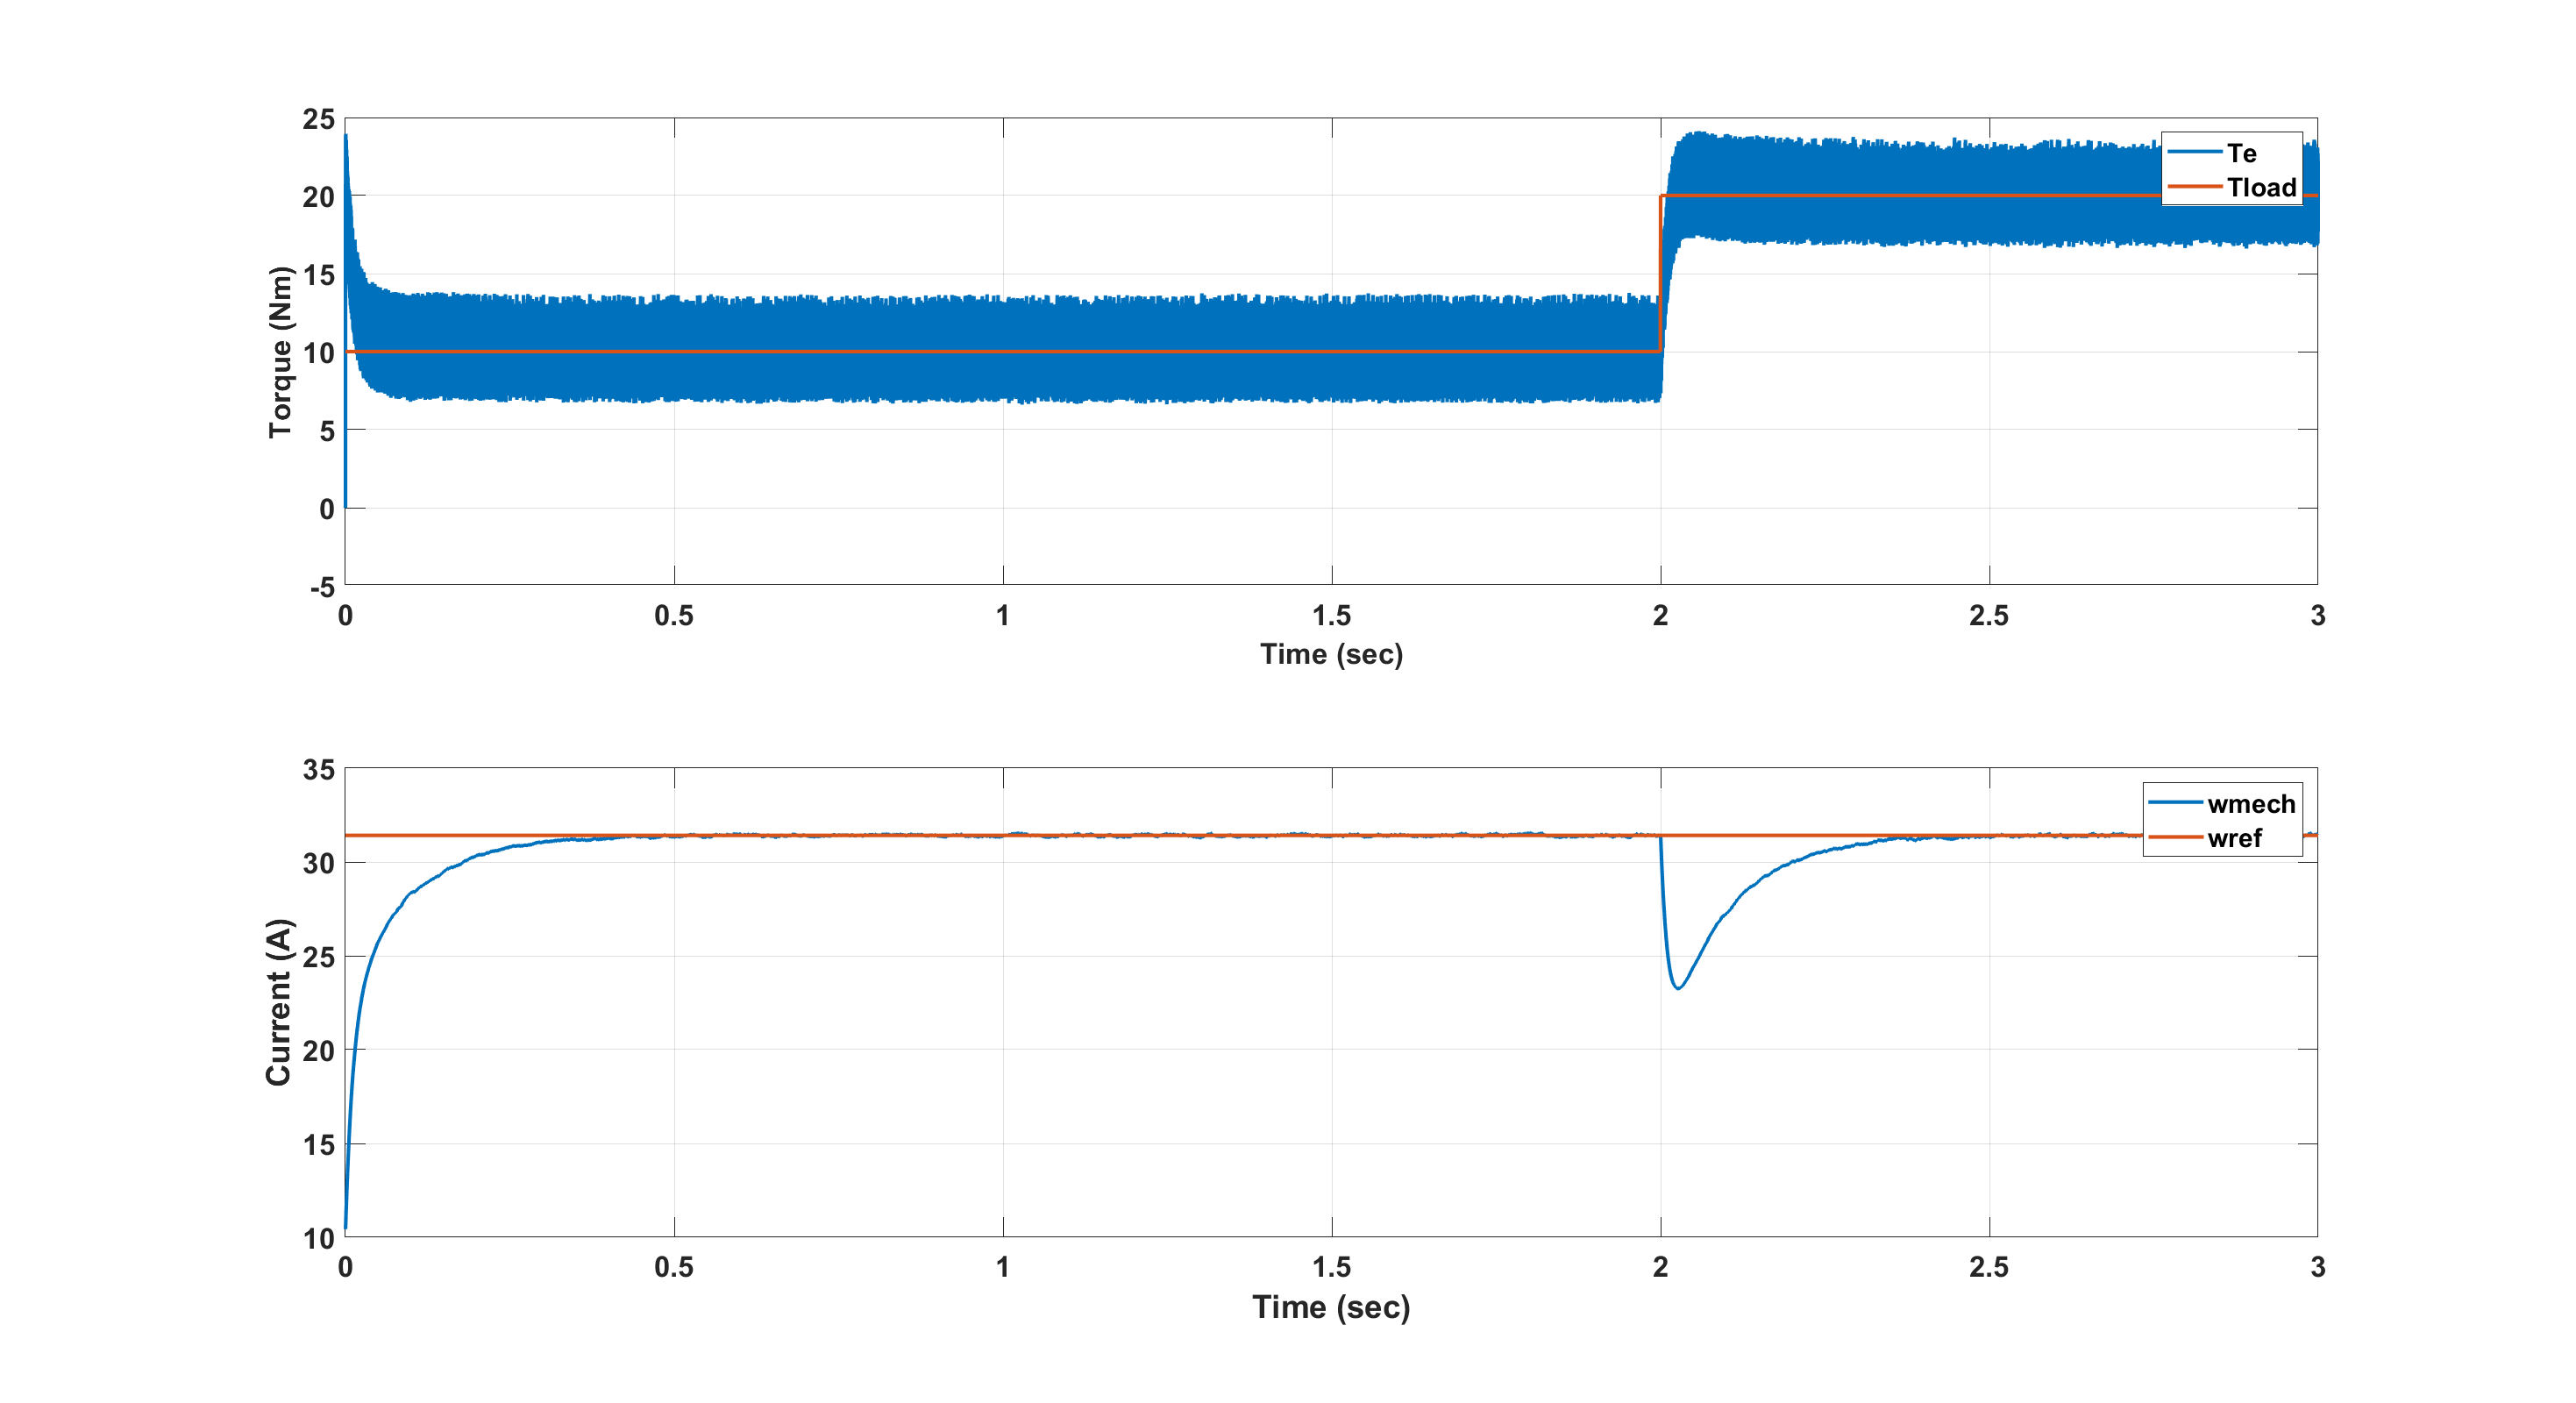
\includegraphics[scale=0.3]{Figures/OneModule/Tload_Wshaft.eps}
\caption{Torque and Rotor Speed for One Module}
\label{fig:Tload_Wshaft_OneModule}
\end{figure}
\begin{figure}[H]
\centering
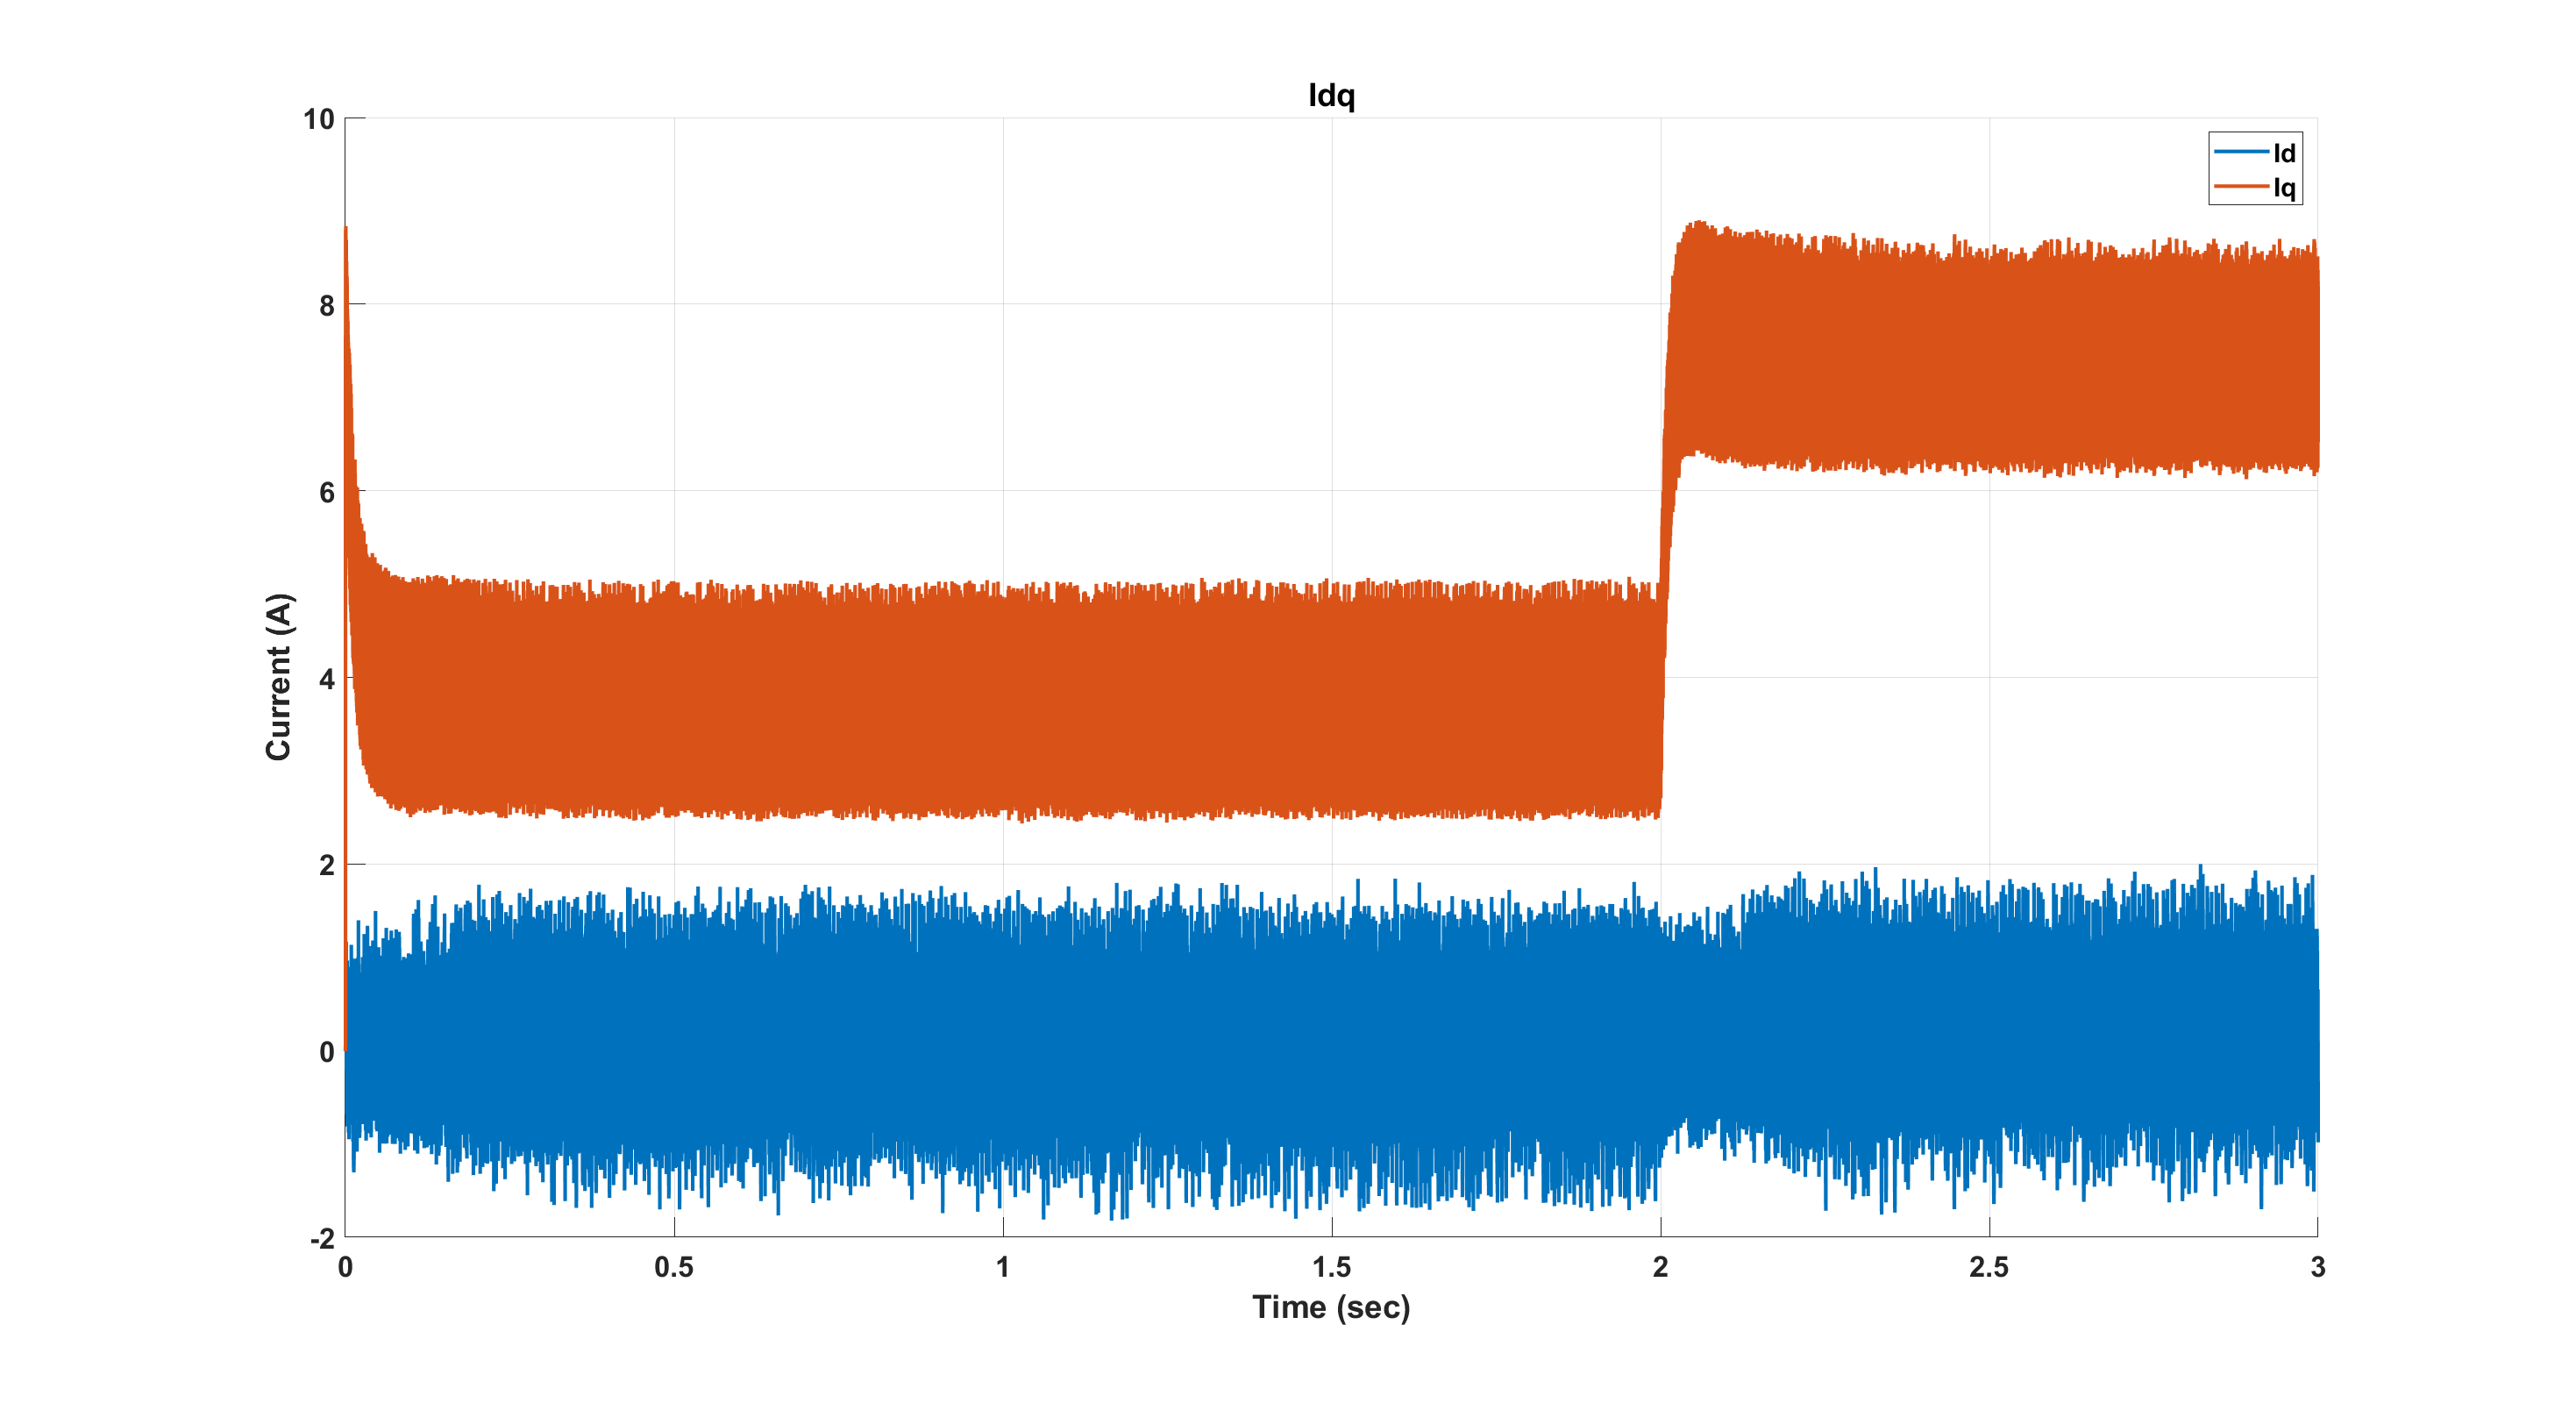
\includegraphics[scale=0.3]{Figures/OneModule/Id_Iq.eps}
\caption{Id Iq for One Module}
\label{fig:Current_dq_OneModule}
\end{figure}
\begin{figure}[H]
\centering
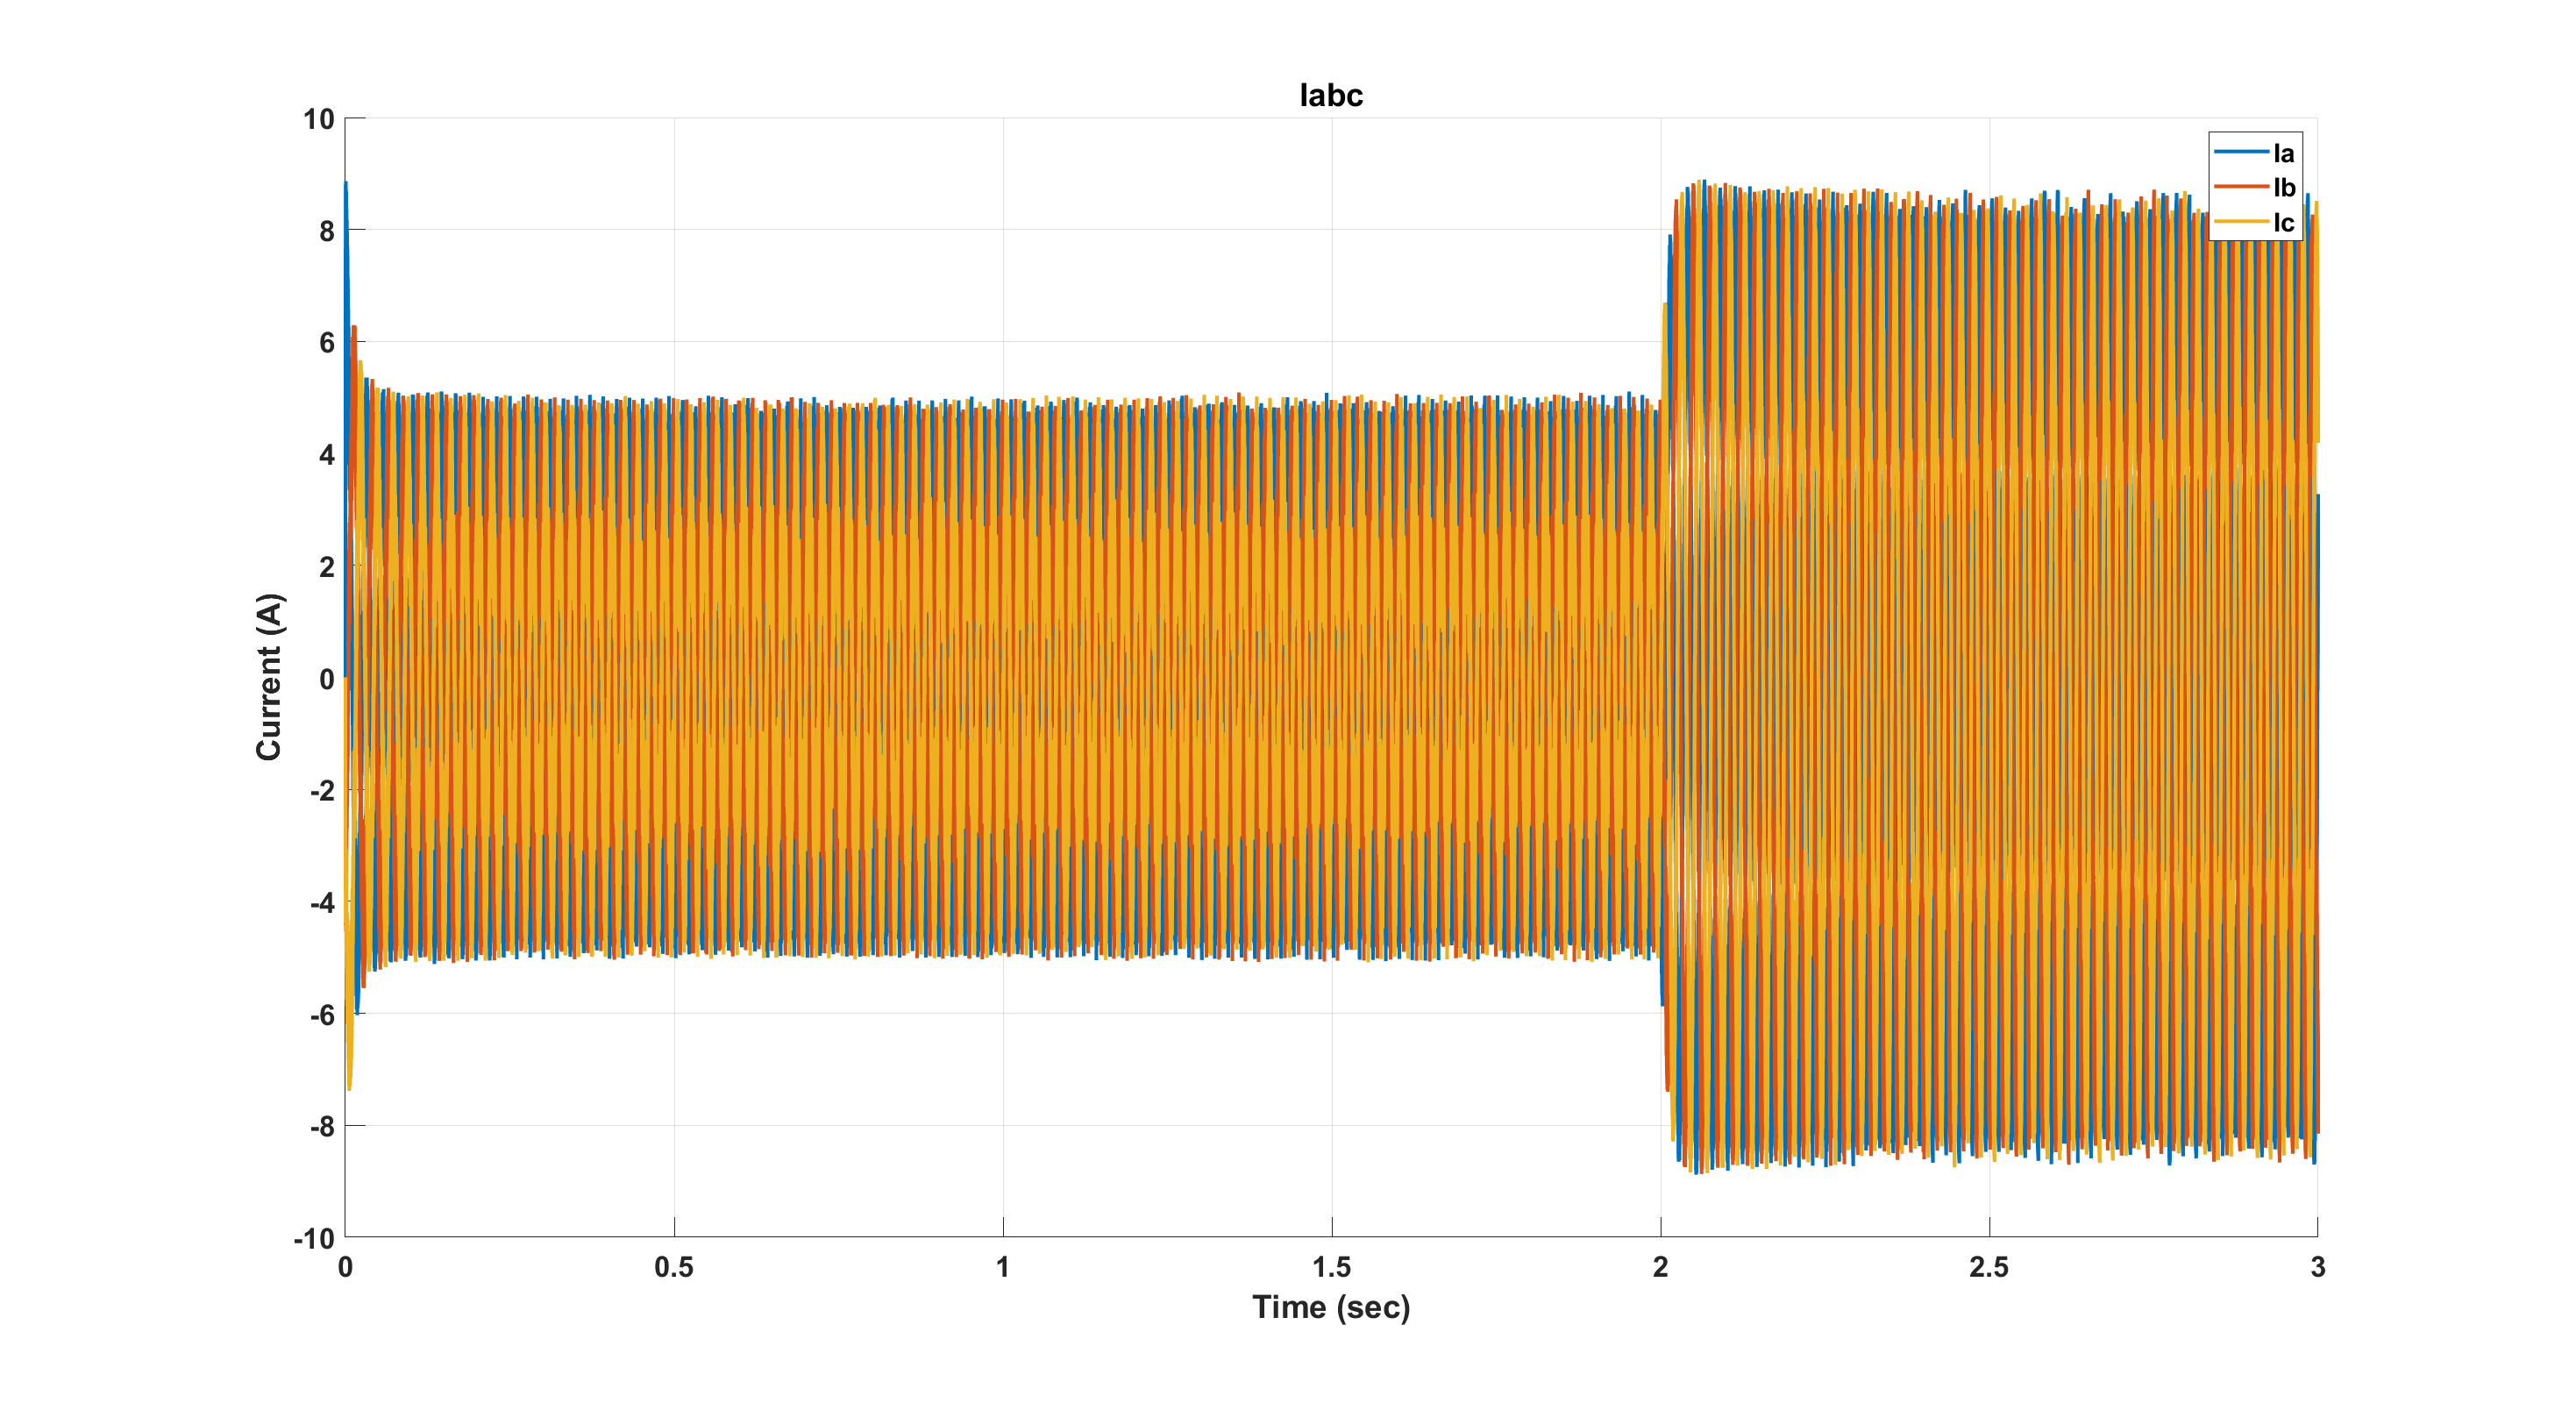
\includegraphics[scale=0.3]{Figures/OneModule/Ia_Ib_Ic.eps}
\caption{Phase Currents for One Module}
\label{fig:Current_abc_OneModule}
\end{figure}



\section{Two Module Implementation}

The configuration of the two module implementation is provided in Figure \ref{fig:DriveSystem}. There are two 3-phase winding groups that are contributing the torque. In construction of this model, first the cost functions are evaluated seperately for each module. 

\begin{figure}[H]
\centering
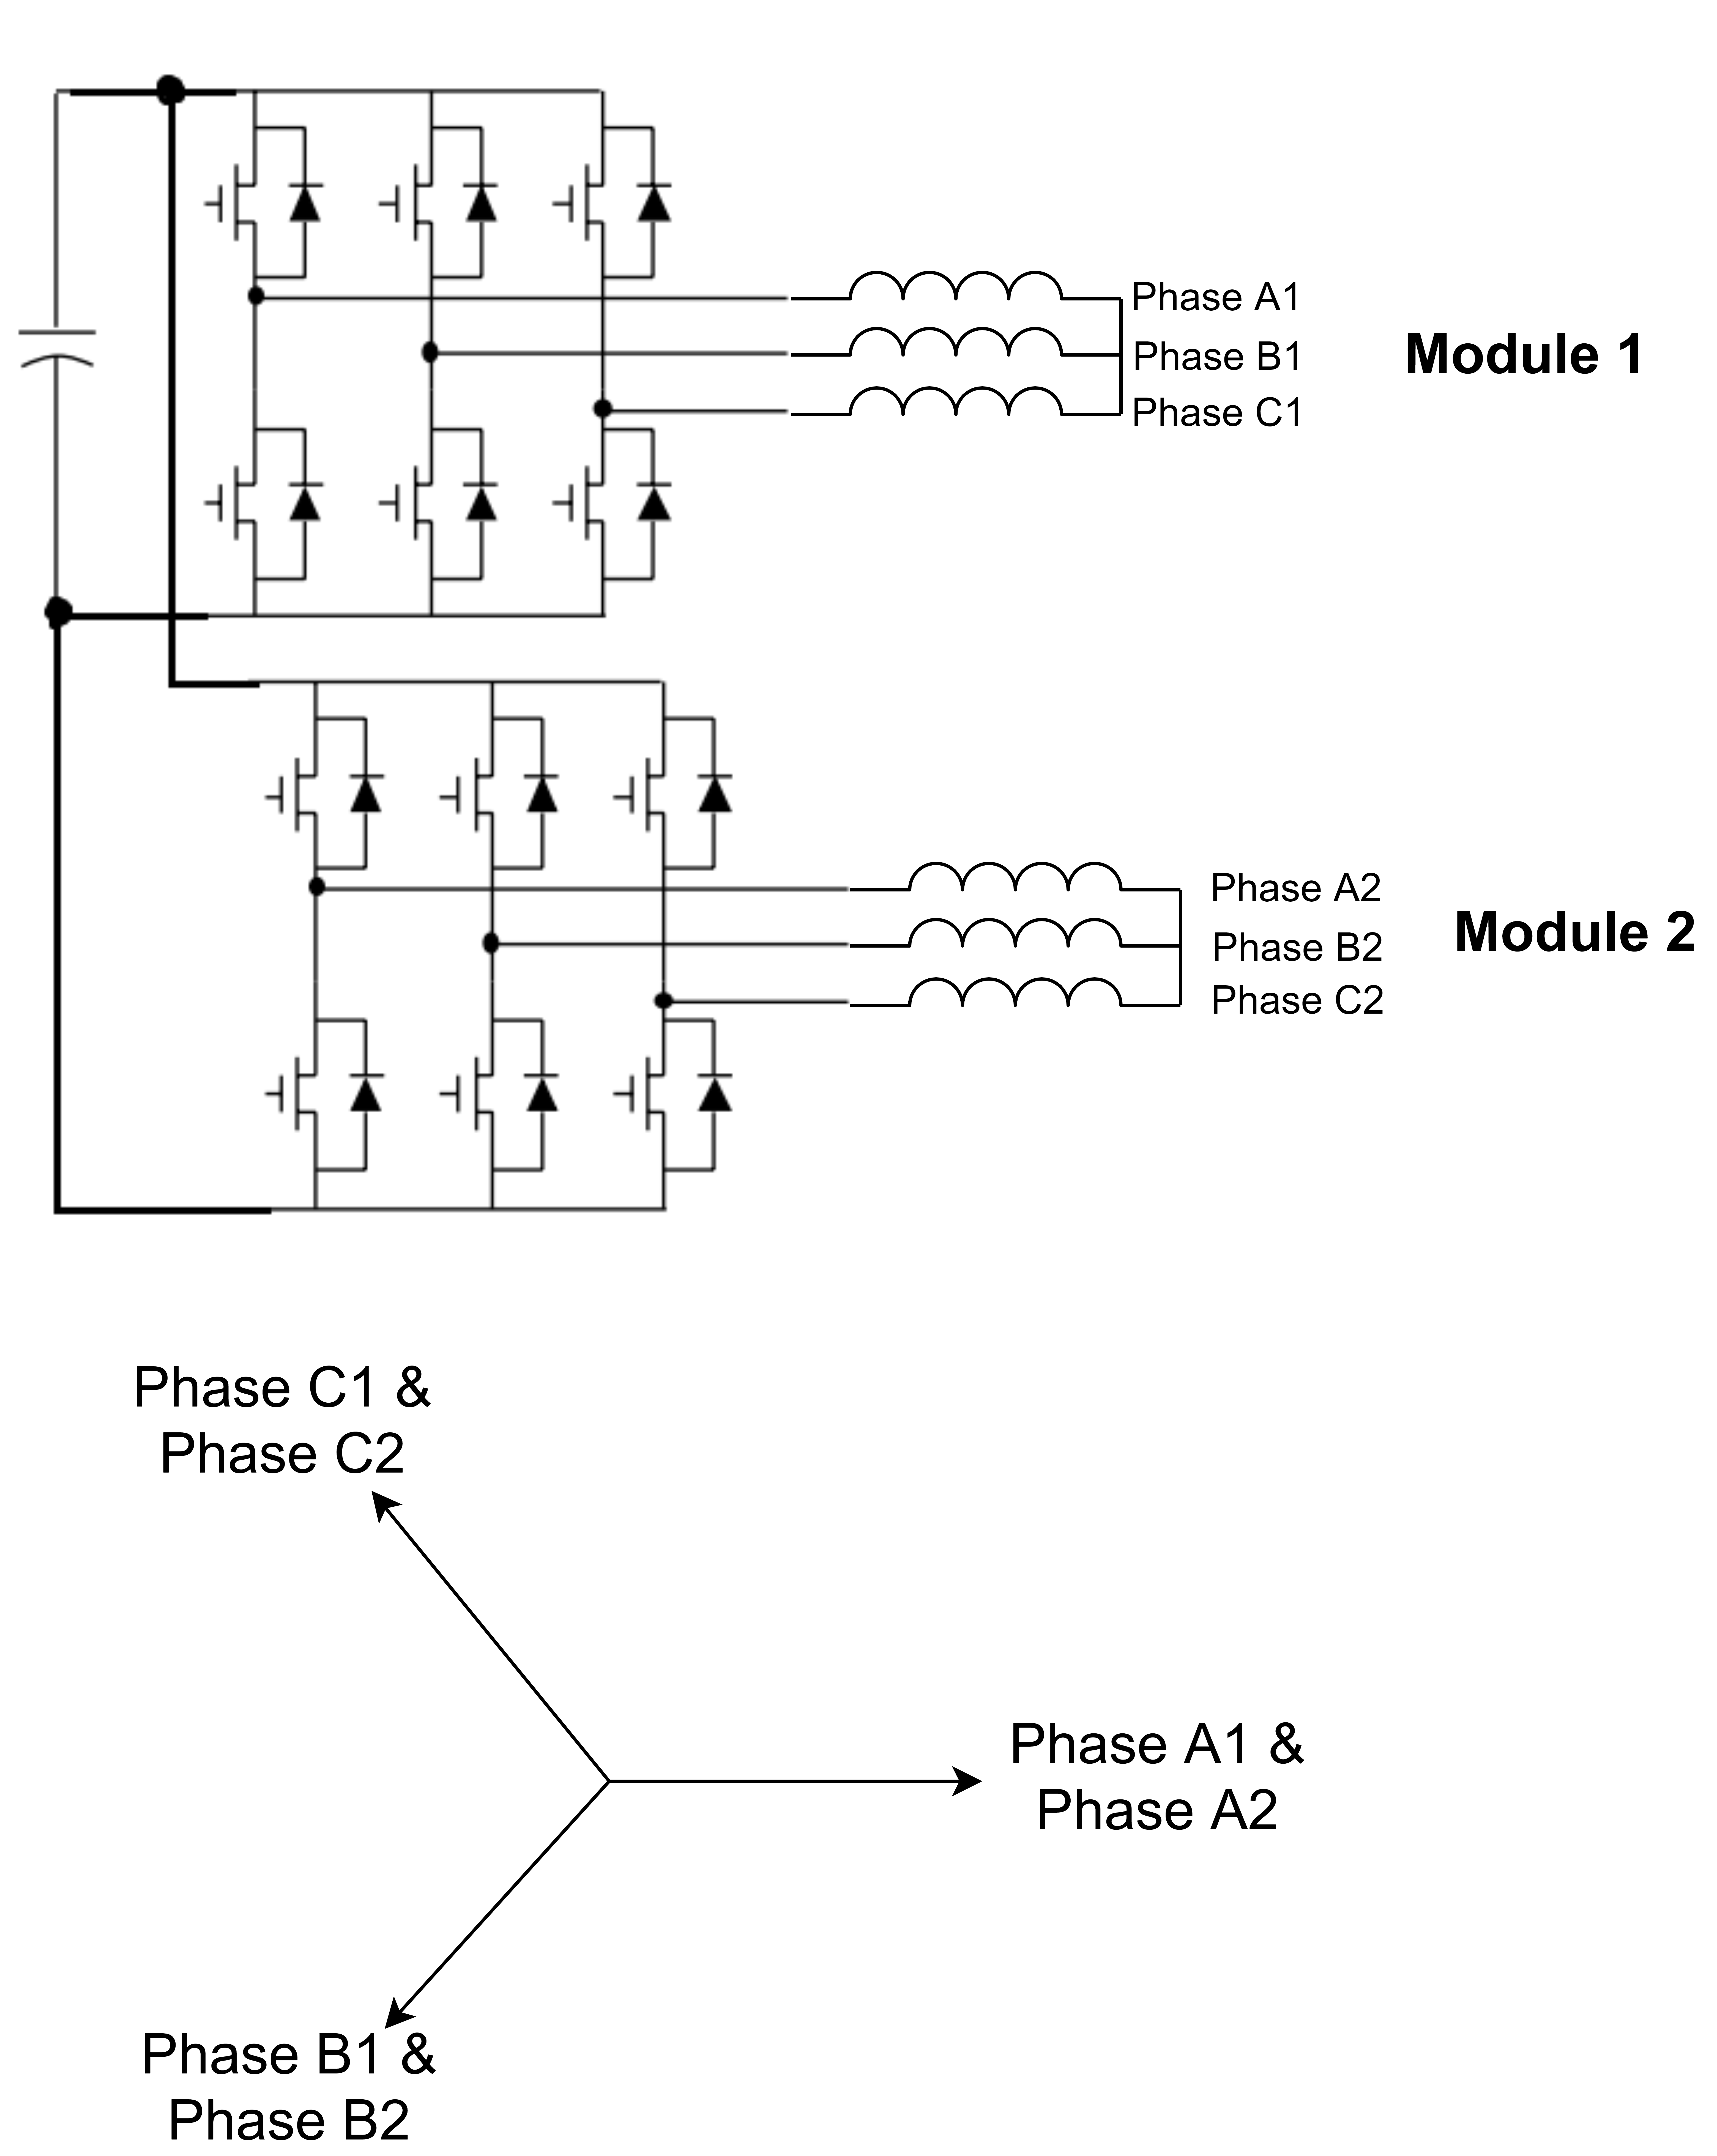
\includegraphics[scale=0.6]{Figures/Drive_System.png}
\caption{The drive circuity and winding configuration}
\label{fig:DriveSystem}
\end{figure}

\newpage

The simulink model is consists of two PMSMs whose shafts are attached to each other, as can be seen in Figure \ref{fig:TwoModuleSimulinkModel}. That way, the machines have the same angular speed and position during the simulation.

\begin{figure}[H]
\centering
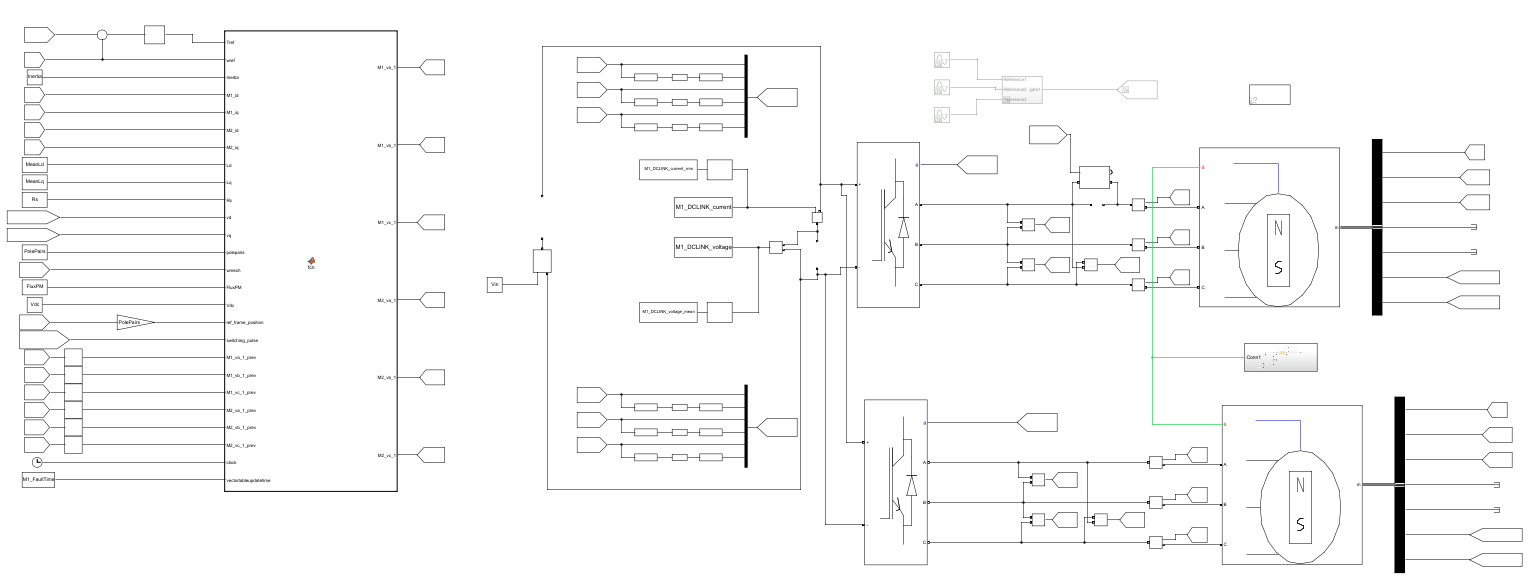
\includegraphics[scale=0.4]{Figures/TwoModuleSimulinkModel.PNG}
\caption{Two Module Simulink Model}
\label{fig:TwoModuleSimulinkModel}
\end{figure}

For two module configuration, the cost function has been evaluated with different configurations. These are:
\begin{itemize}
    \item Seperate cost functions for each module
    \item Combined cost function with the same switching vectors evaluated
    \item Combined cost function with all switching combinations evaluated
\end{itemize}

\subsection{Seperate Cost Functions for Each Module}
The seperate cost functions can be seen in line \ref{line:Two_Module_cost1} and line \ref{line:Two_Module_cost2} of Listing \ref{code:TwoModuleSeperateCost}. 


\subsubsection{Healthy Operation}


It can be seen from Figures \ref{fig:Tload_TwoModuleSeperateCost}, \ref{fig:Wshaft_TwoModuleSeperateCost}, \ref{fig:Current_dq_TwoModuleSeperateCost}, \ref{fig:Current_abc_TwoModuleSeperateCost}, that the steady state operation is achieved for seperate cost functions. However, the torque ripple is still considerably high for both modules.



\begin{figure}[H]
\centering
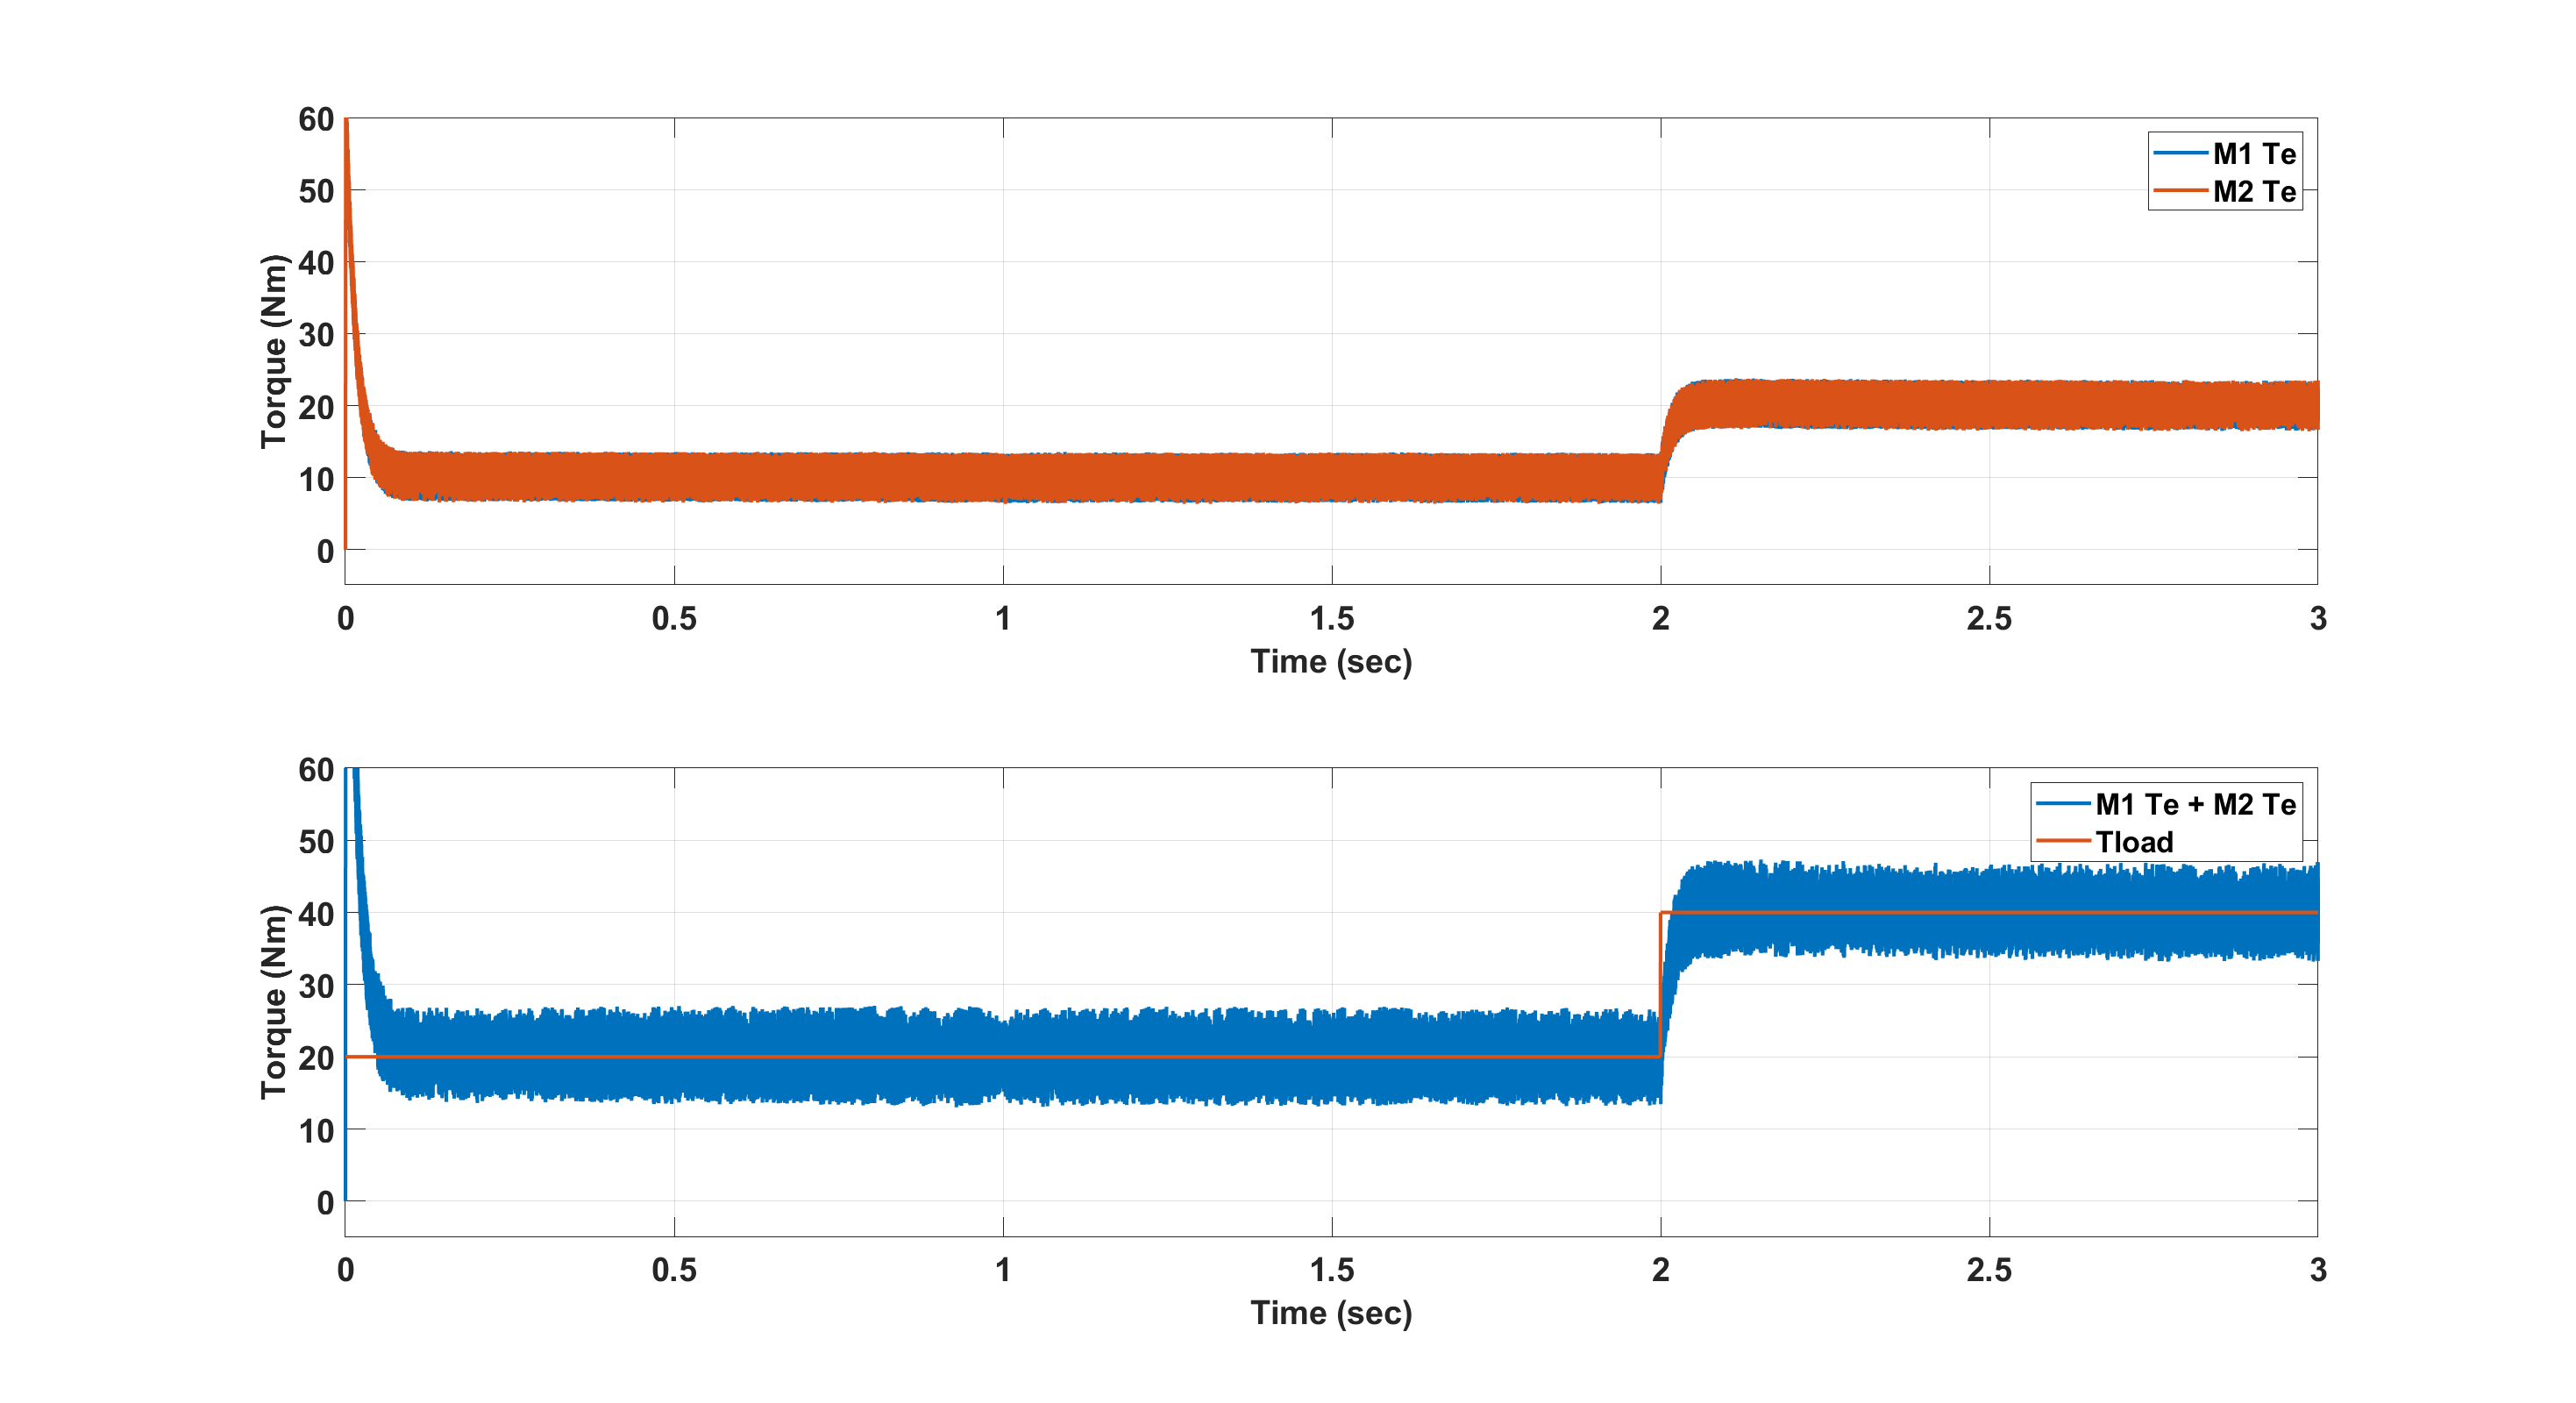
\includegraphics[scale=0.3]{Figures/TwoModule/SeperateCost/Torques.eps}
\caption{Torque generation of each module with seperate cost functions with no open circuit fault}
\label{fig:Tload_TwoModuleSeperateCost}
\end{figure}
\begin{figure}[H]
\centering
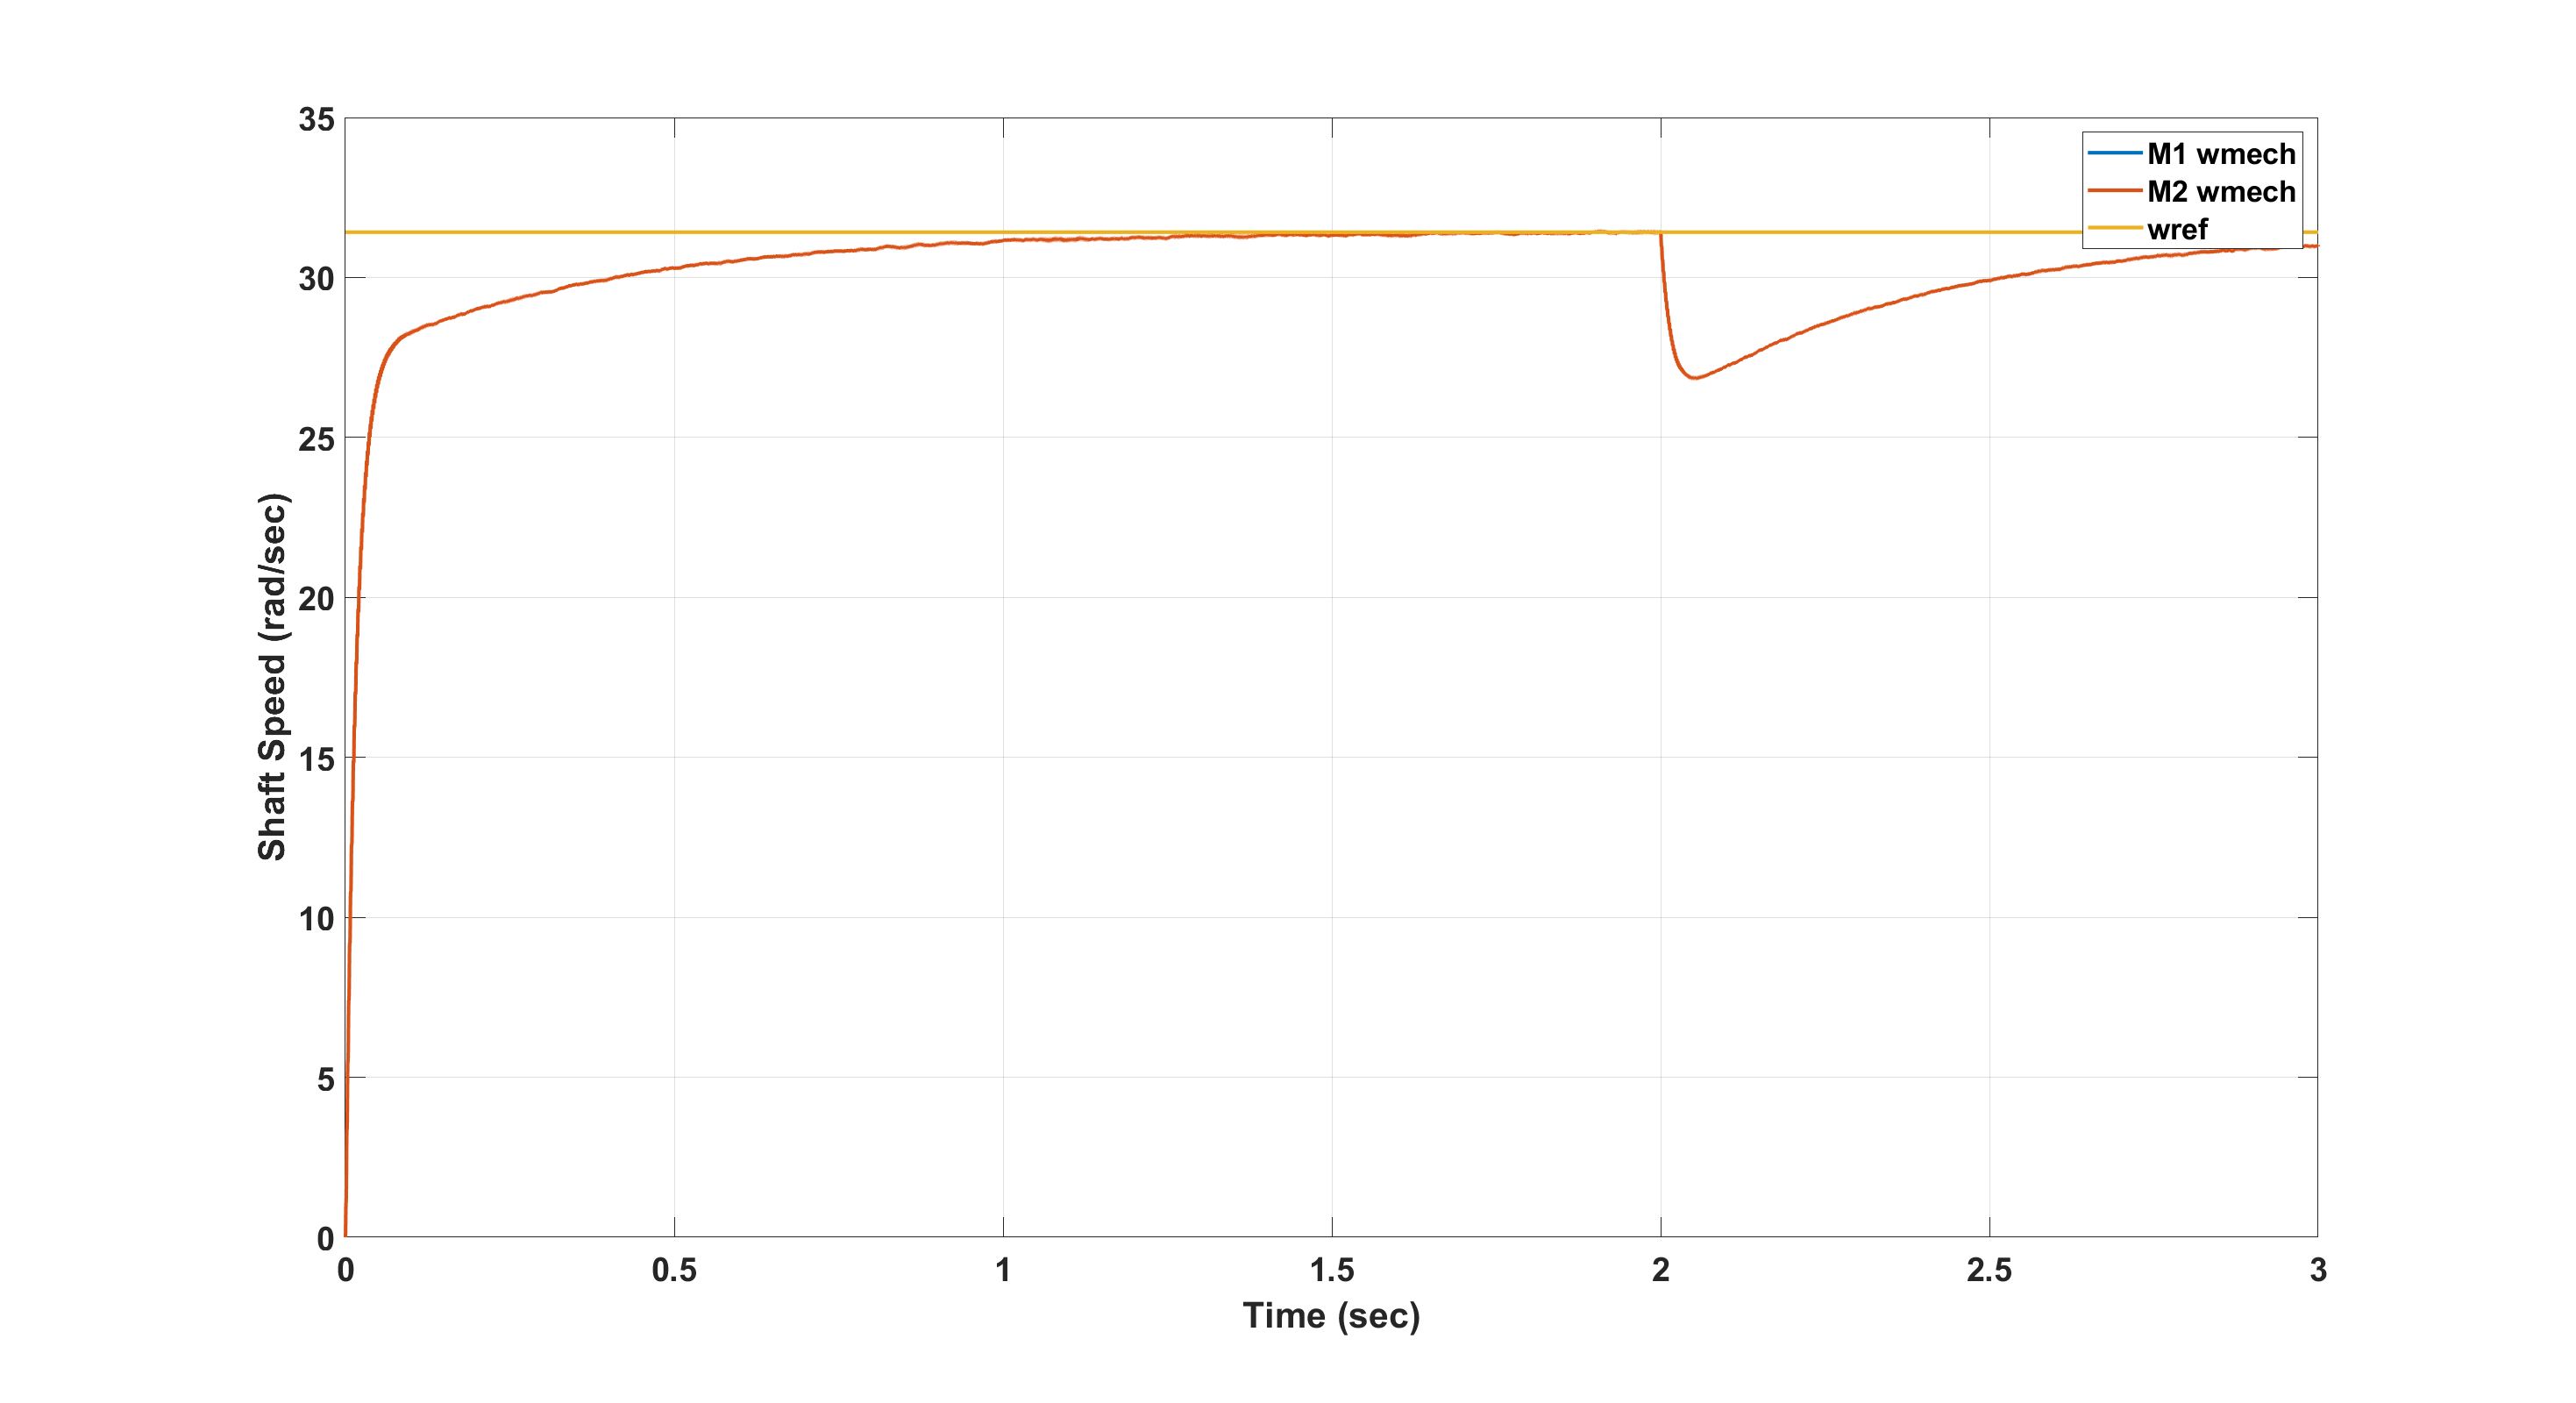
\includegraphics[scale=0.3]{Figures/TwoModule/SeperateCost/ShaftSpeed.eps}
\caption{Shaft speed with seperate cost functions no open circuit fault}
\label{fig:Wshaft_TwoModuleSeperateCost}
\end{figure}
\begin{figure}[H]
\centering
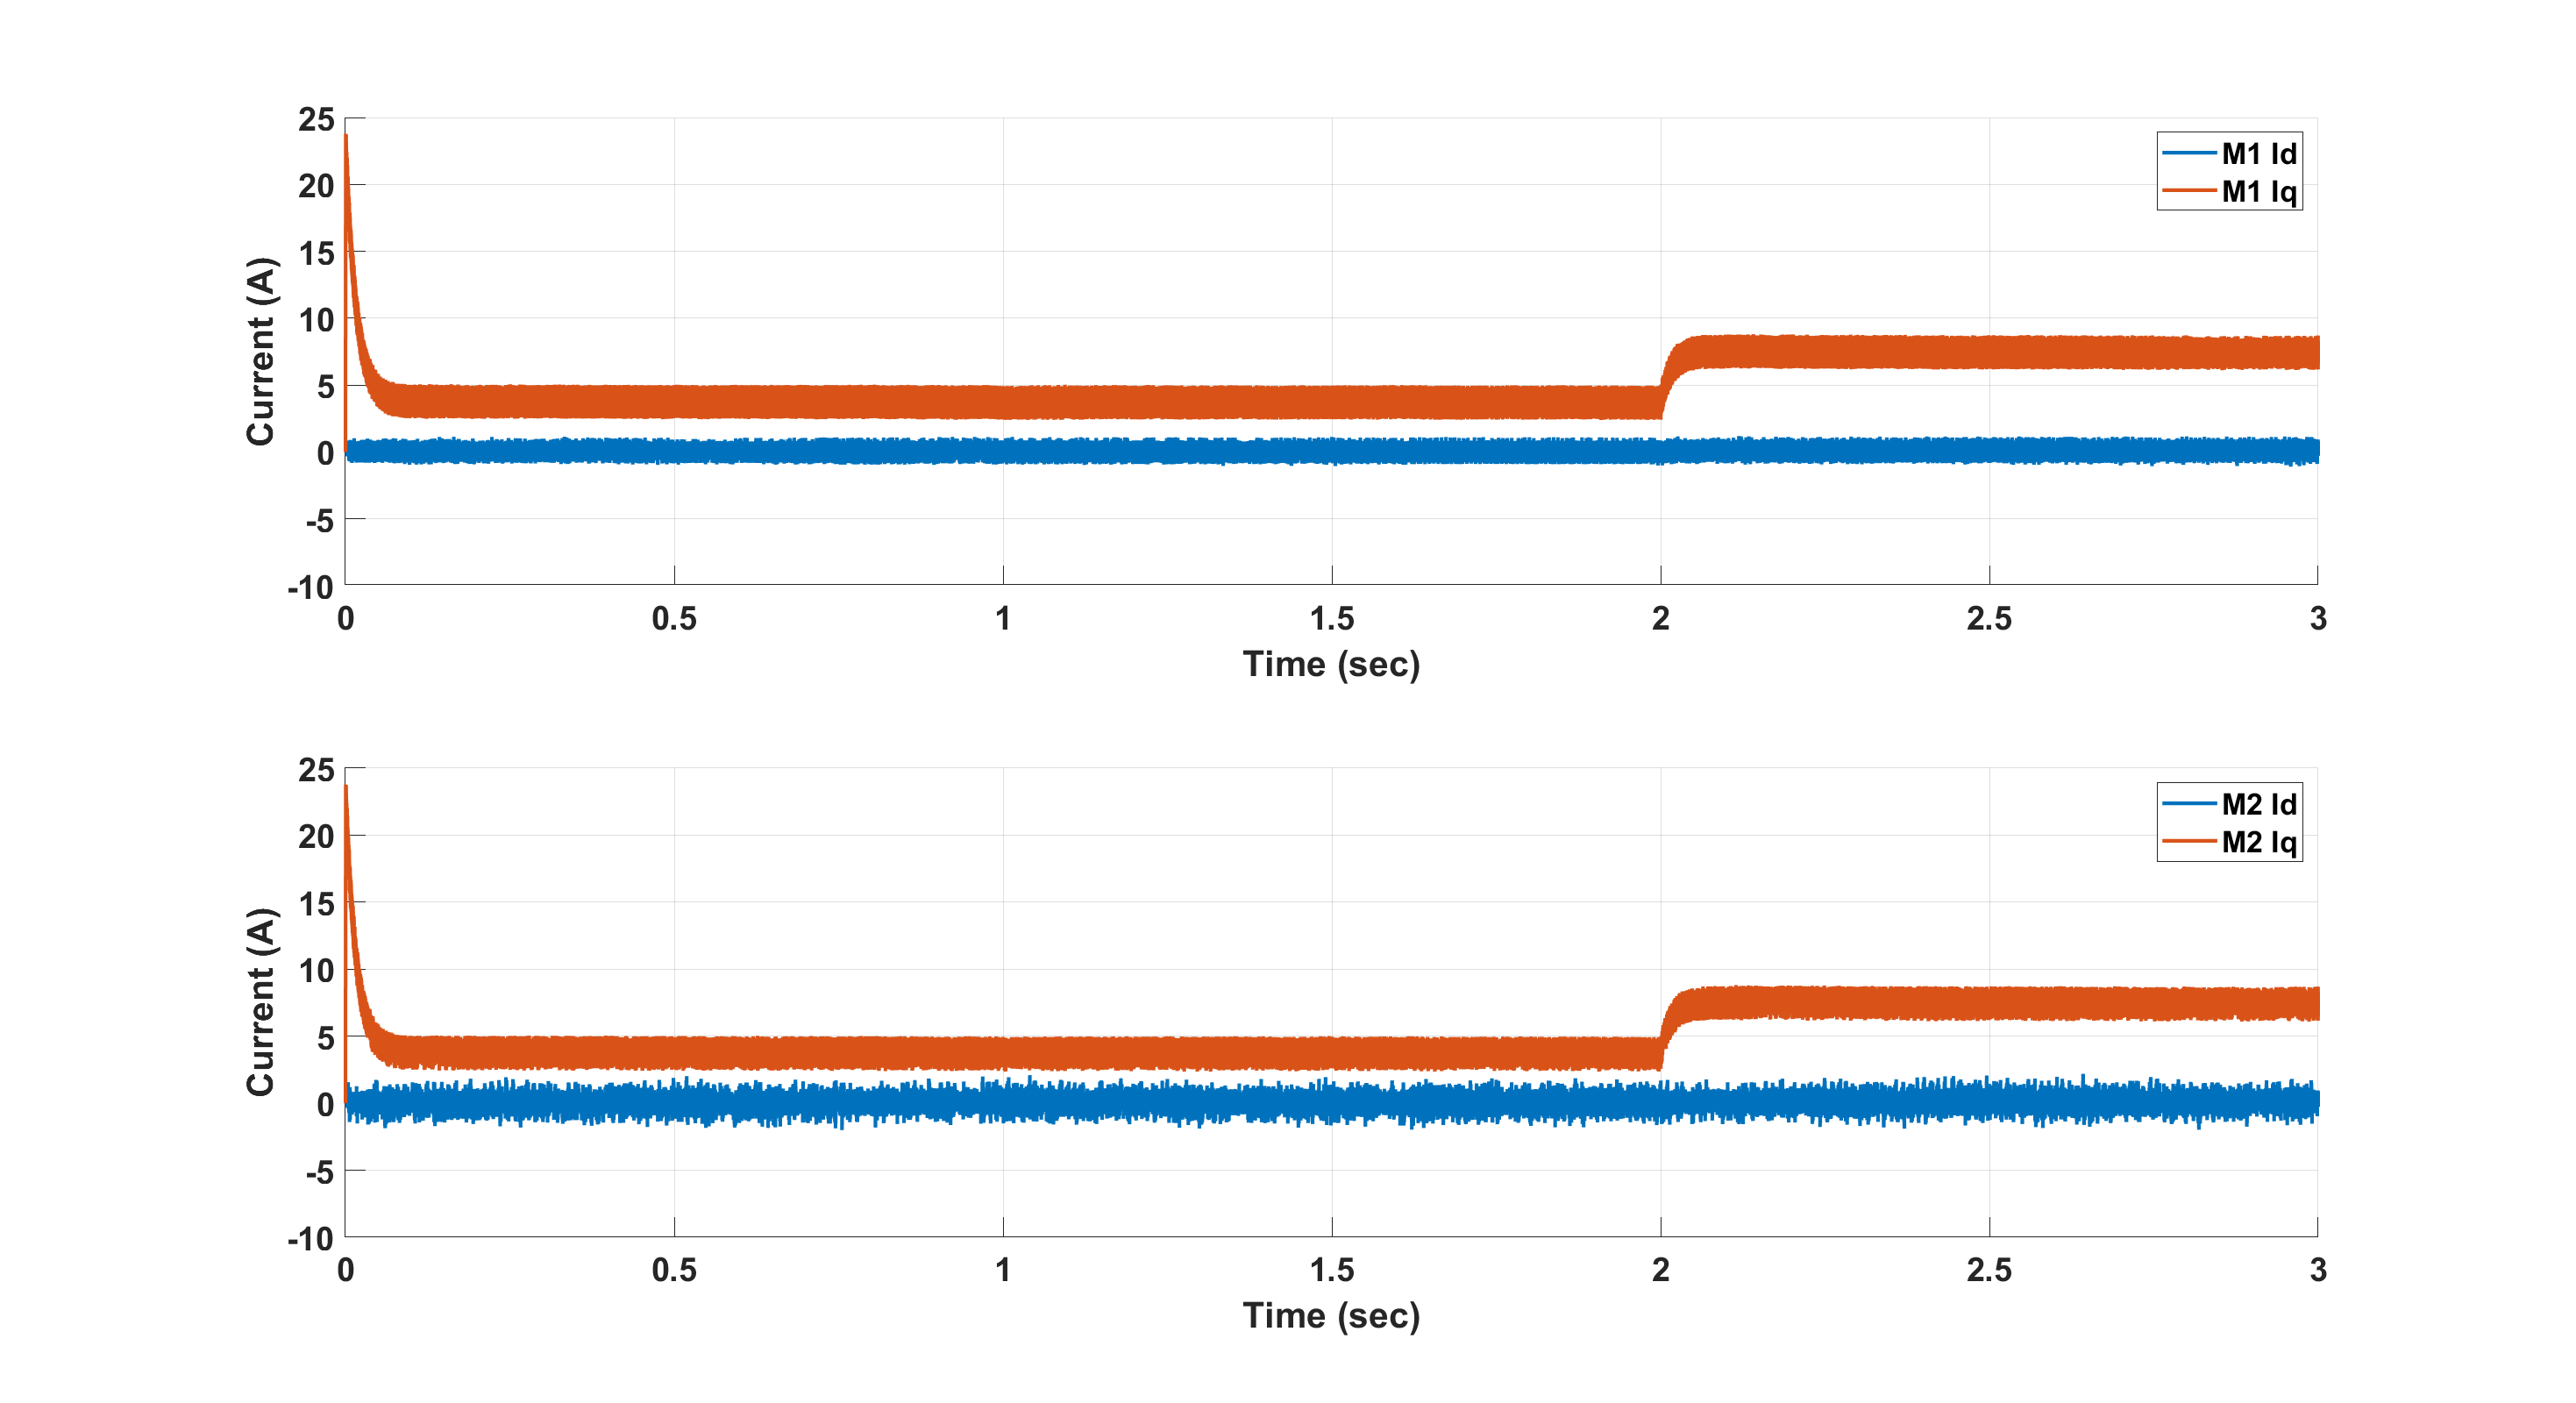
\includegraphics[scale=0.3]{Figures/TwoModule/SeperateCost/Id_Iq.eps}
\caption{Id Iq for Two Modules with seperate cost functions no open circuit fault}
\label{fig:Current_dq_TwoModuleSeperateCost}
\end{figure}
\begin{figure}[H]
\centering
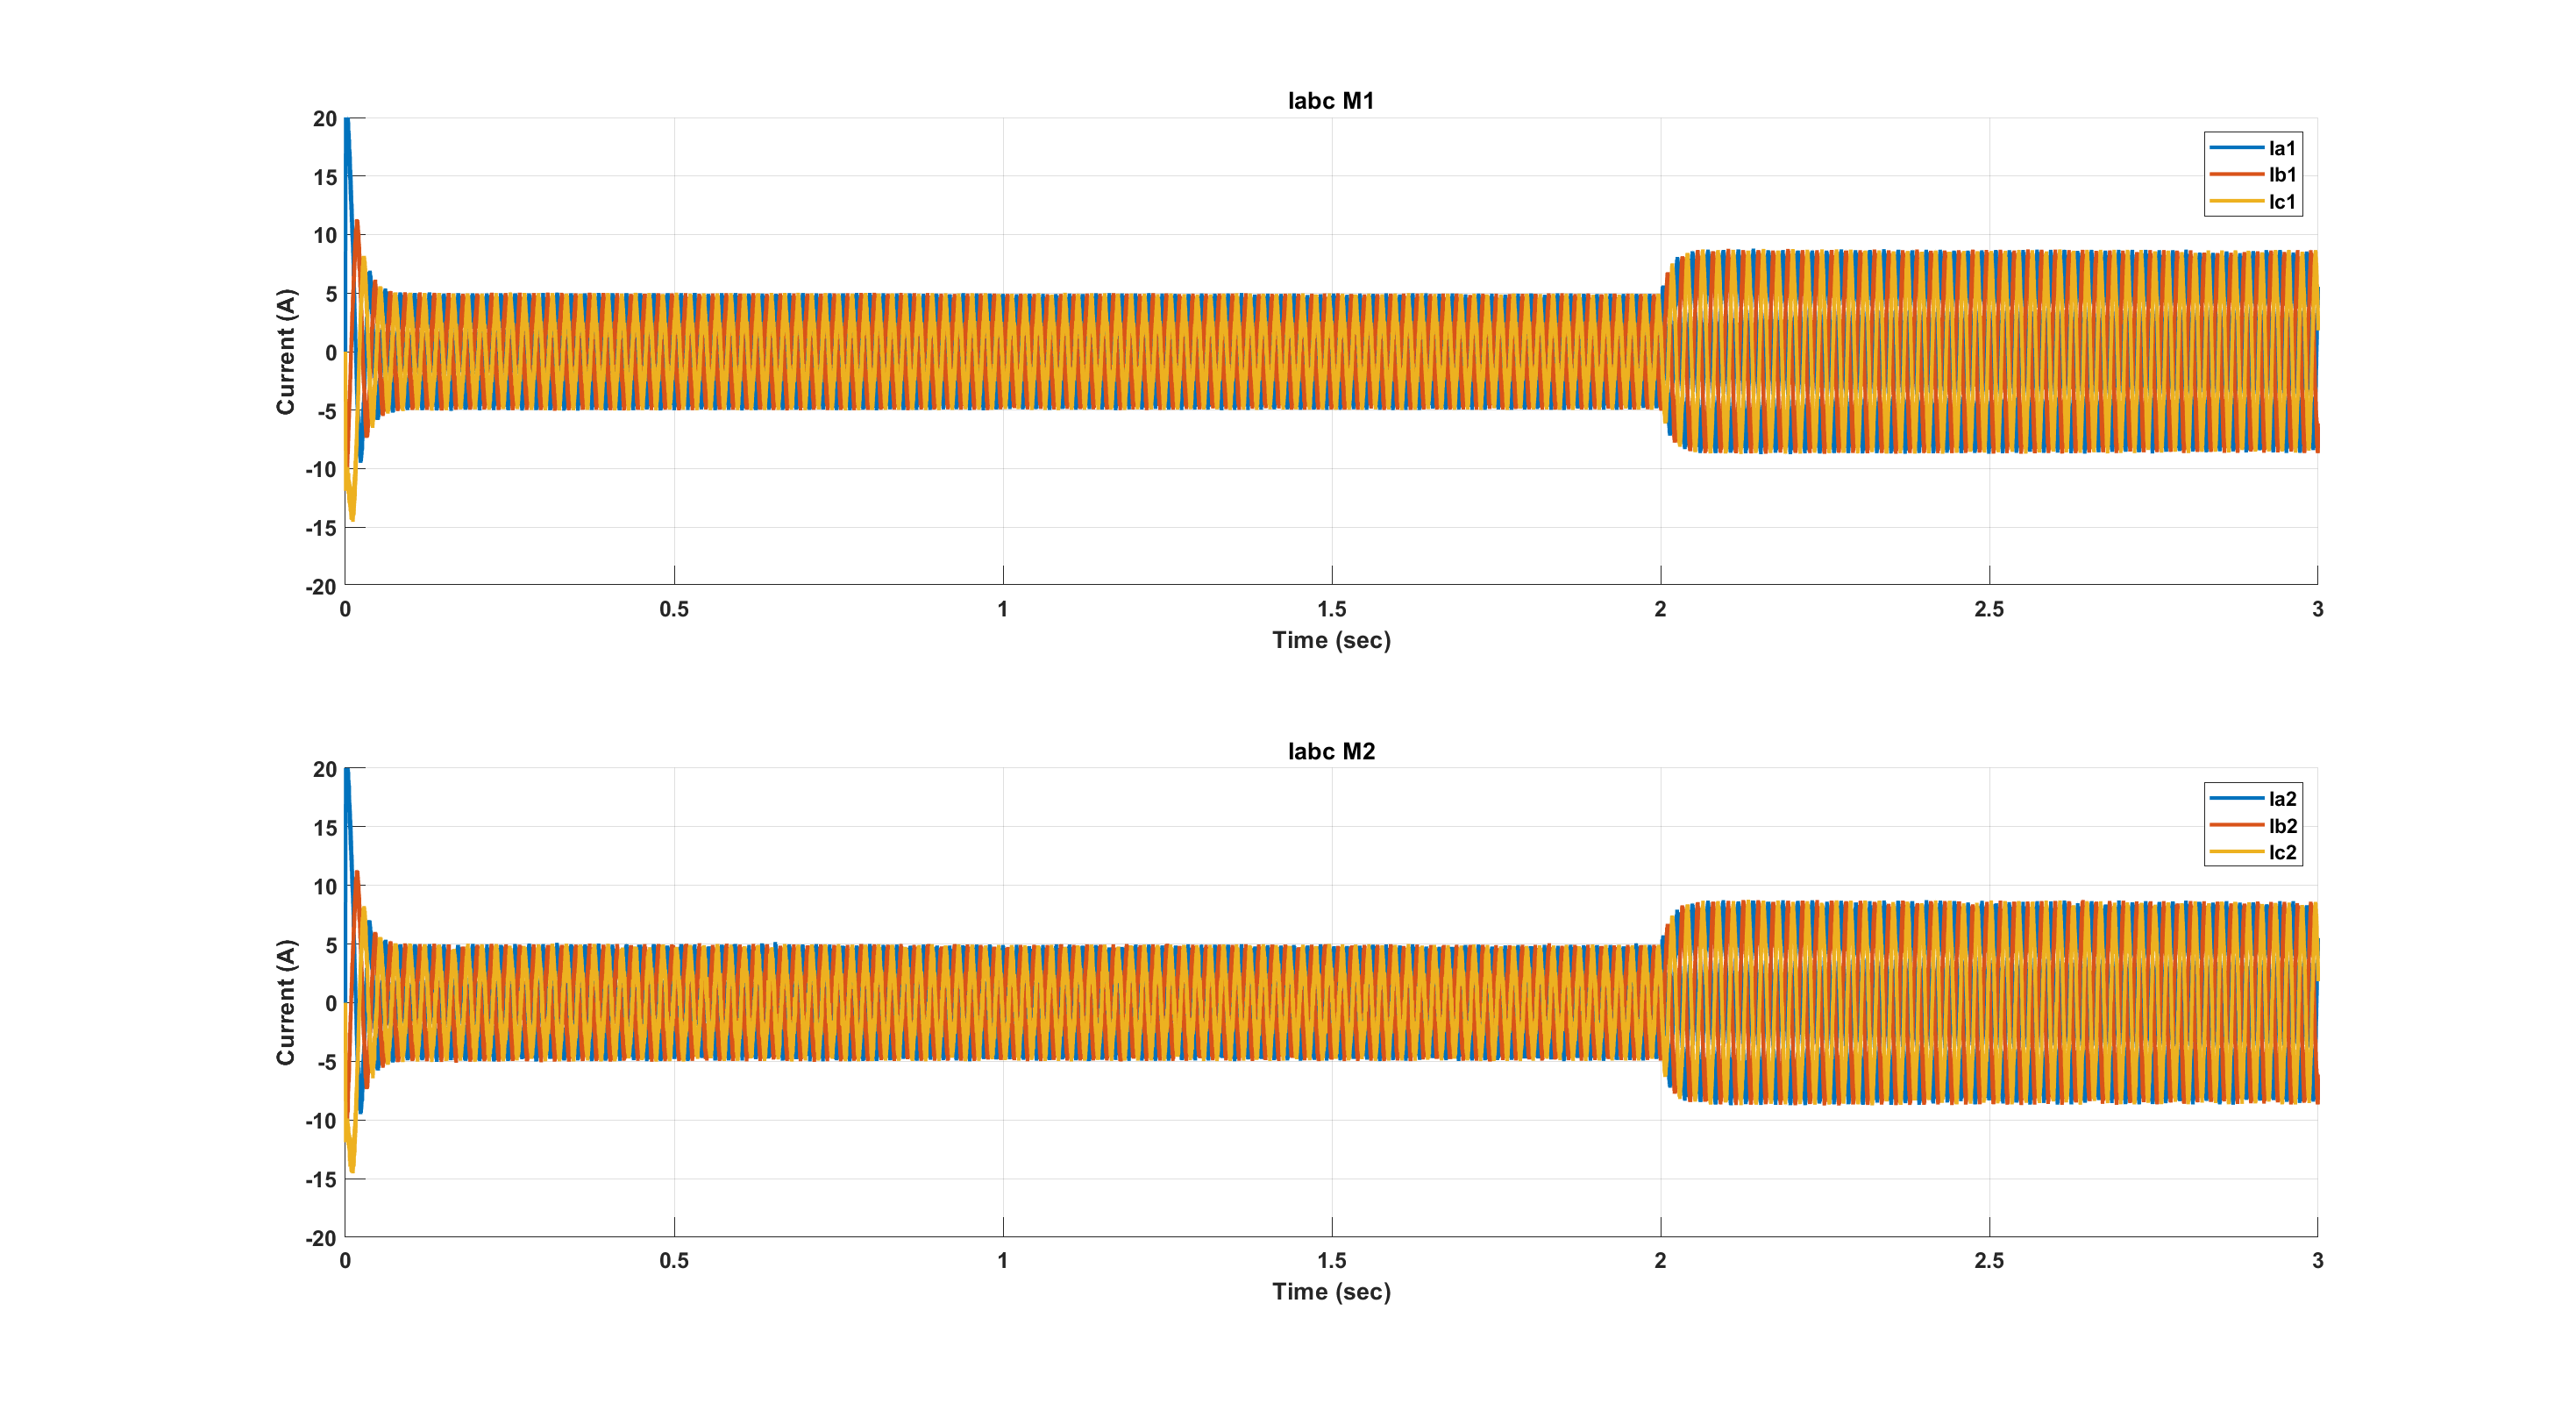
\includegraphics[scale=0.3]{Figures/TwoModule/SeperateCost/Ia_Ib_Ic.eps}
\caption{Phase Currents for Two Modules with seperate cost functions no open circuit fault}
\label{fig:Current_abc_TwoModuleSeperateCost}
\end{figure}
\subsubsection{Faulty Operation}
Even though this approach is suitable for steady state operations, the fault performance is not as expected. The reason is that, since each module is evaluated seperately, each module tries to optimize its own parameters. During the fault, the torque ripple of the faulty module directly added to the shaft torque which not desired (see Figure \ref{fig:FaultMomentSeperateCost}).

\begin{figure}[H]
\centering
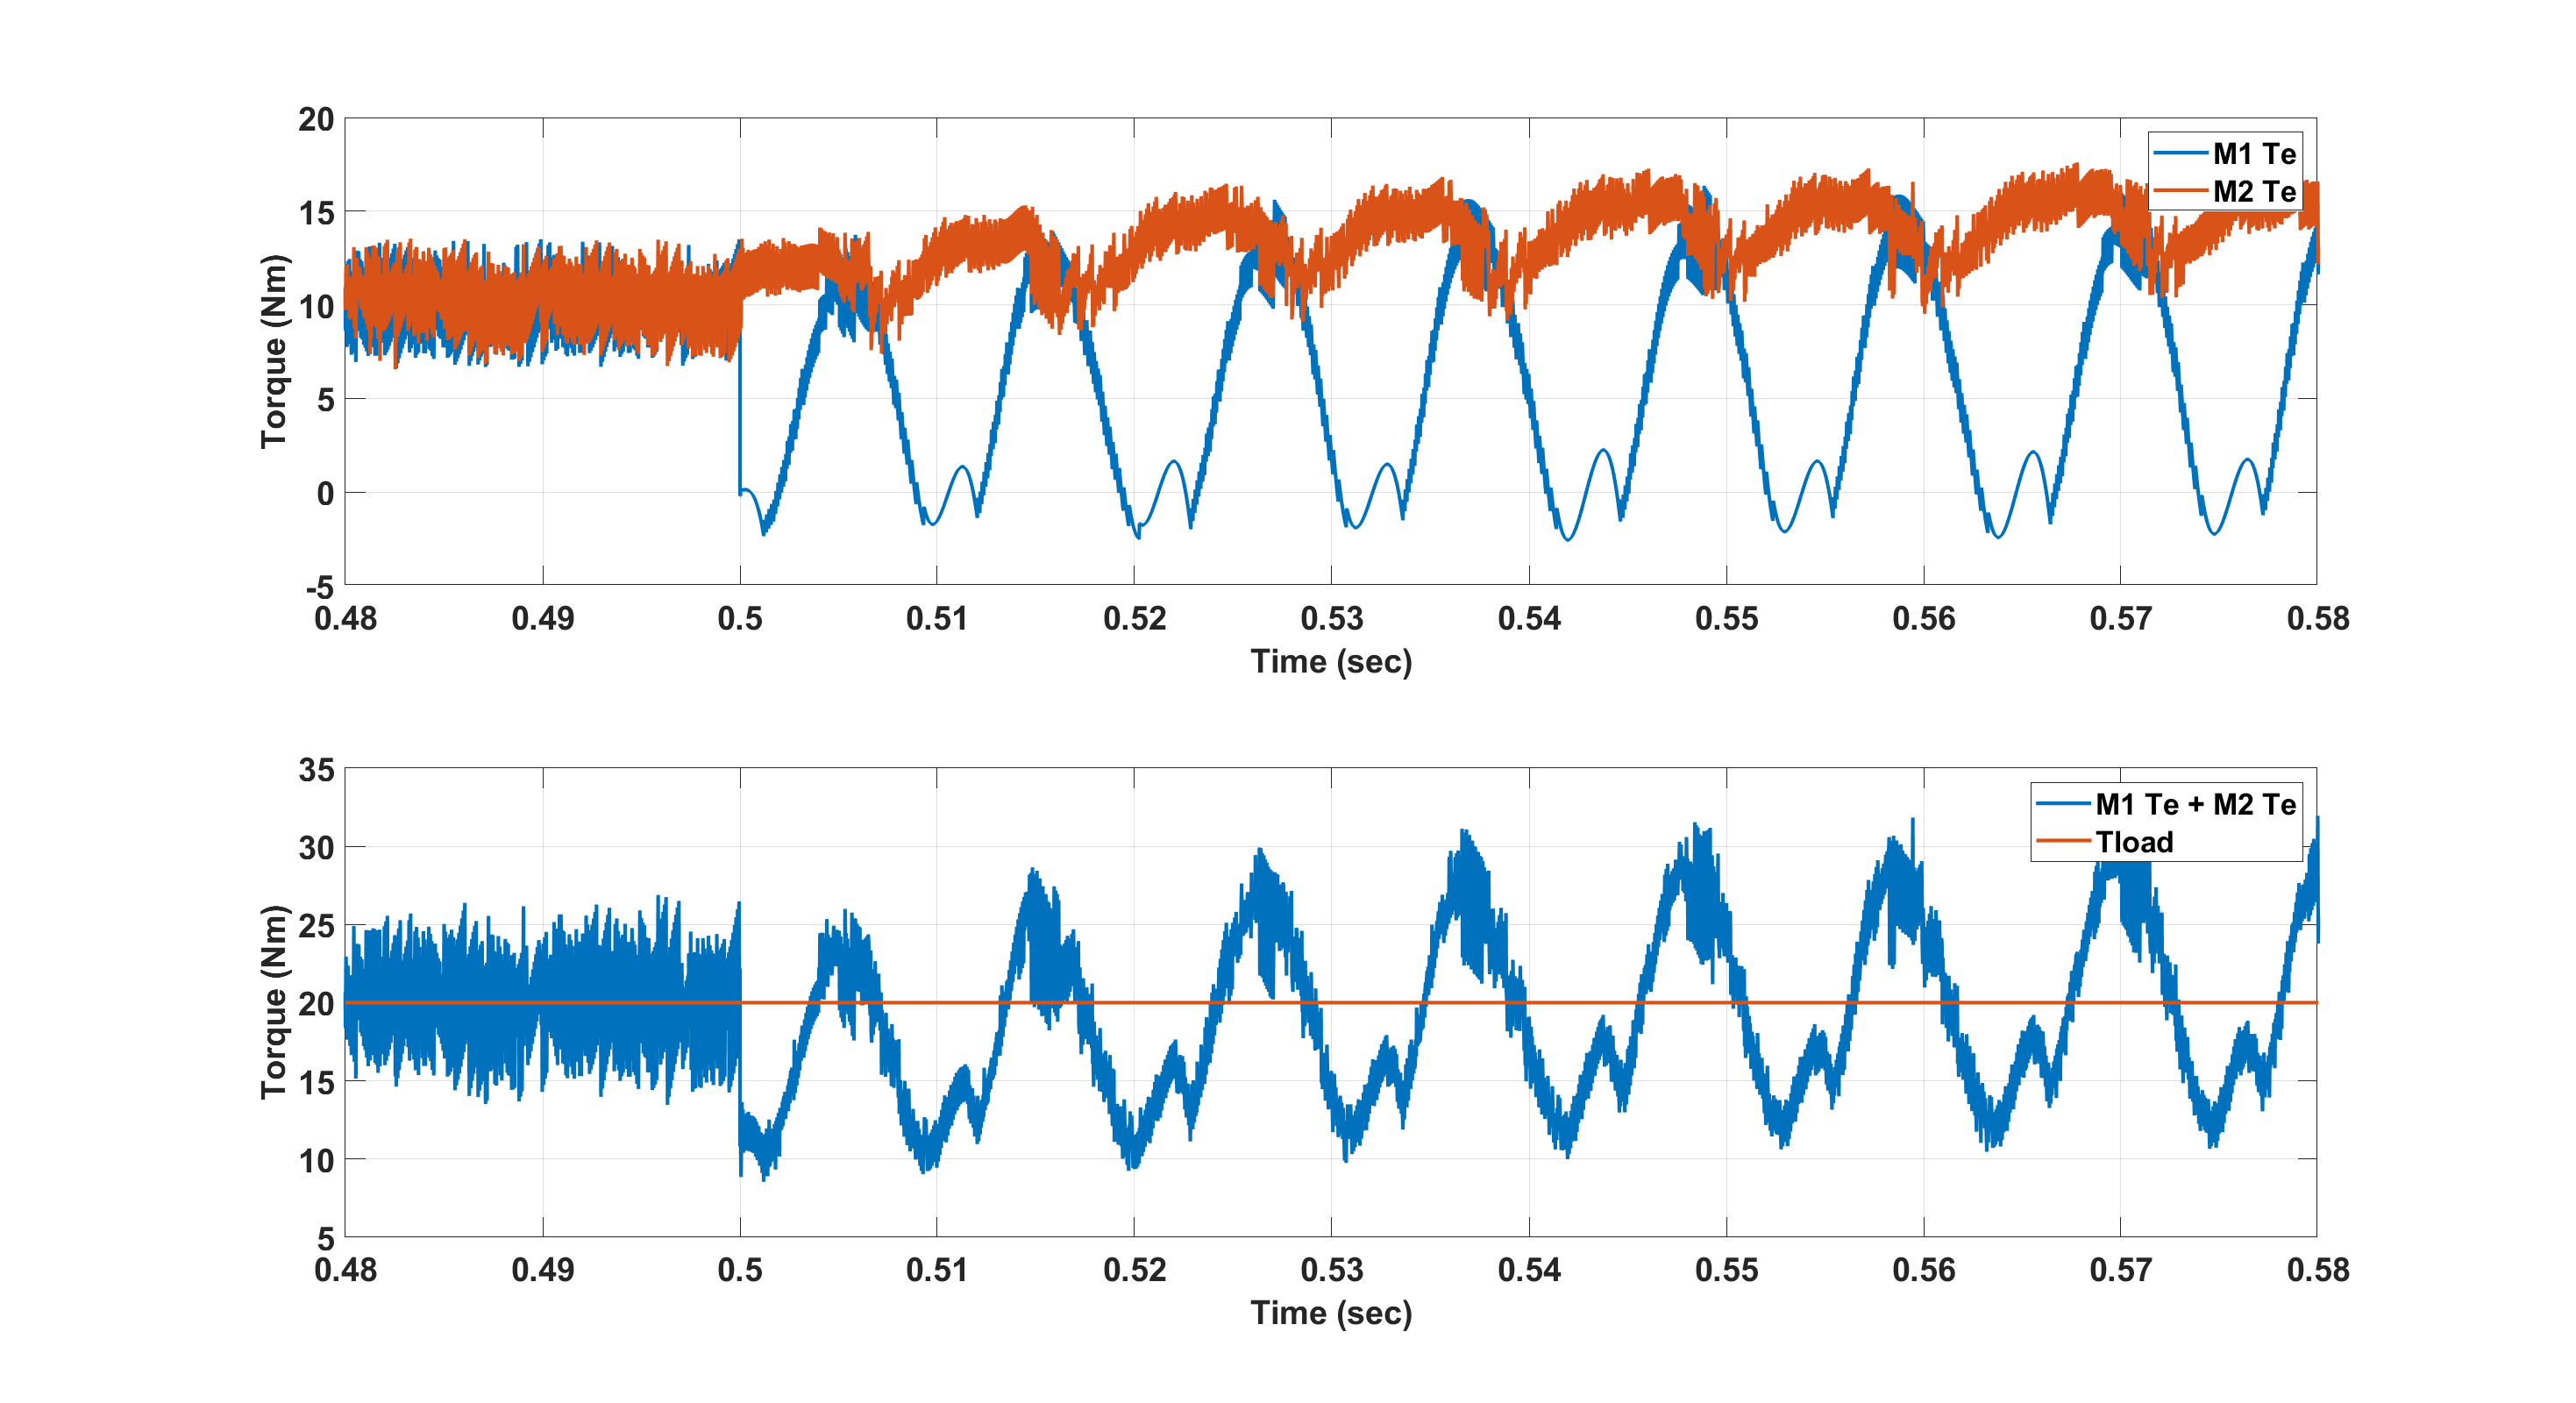
\includegraphics[scale=0.3]{Figures/TwoModule/SeperateCost/FaultMoment.eps}
\caption{Torque Generation at Fault Moment of each module for seperate cost functions}
\label{fig:FaultMomentSeperateCost}
\end{figure}

\subsection{Combined Cost Function}
The combined cost function can be seen in line \ref{line:Two_Module_cost_combined} of Listing \ref{code:TwoModuleCombinedCost}. Note that the combined cost function is evaluated.

\subsubsection{Healthy Operation}
The simulation results for Healthy operation for combined cost function is provided in Figures \ref{fig:Tload_TwoModuleCombinedCost}, \ref{fig:Wshaft_TwoModuleCombinedCost}, \ref{fig:Current_dq_TwoModuleCombinedCost}, \ref{fig:Current_abc_TwoModuleCombinedCost}.



\begin{figure}[H]
\centering
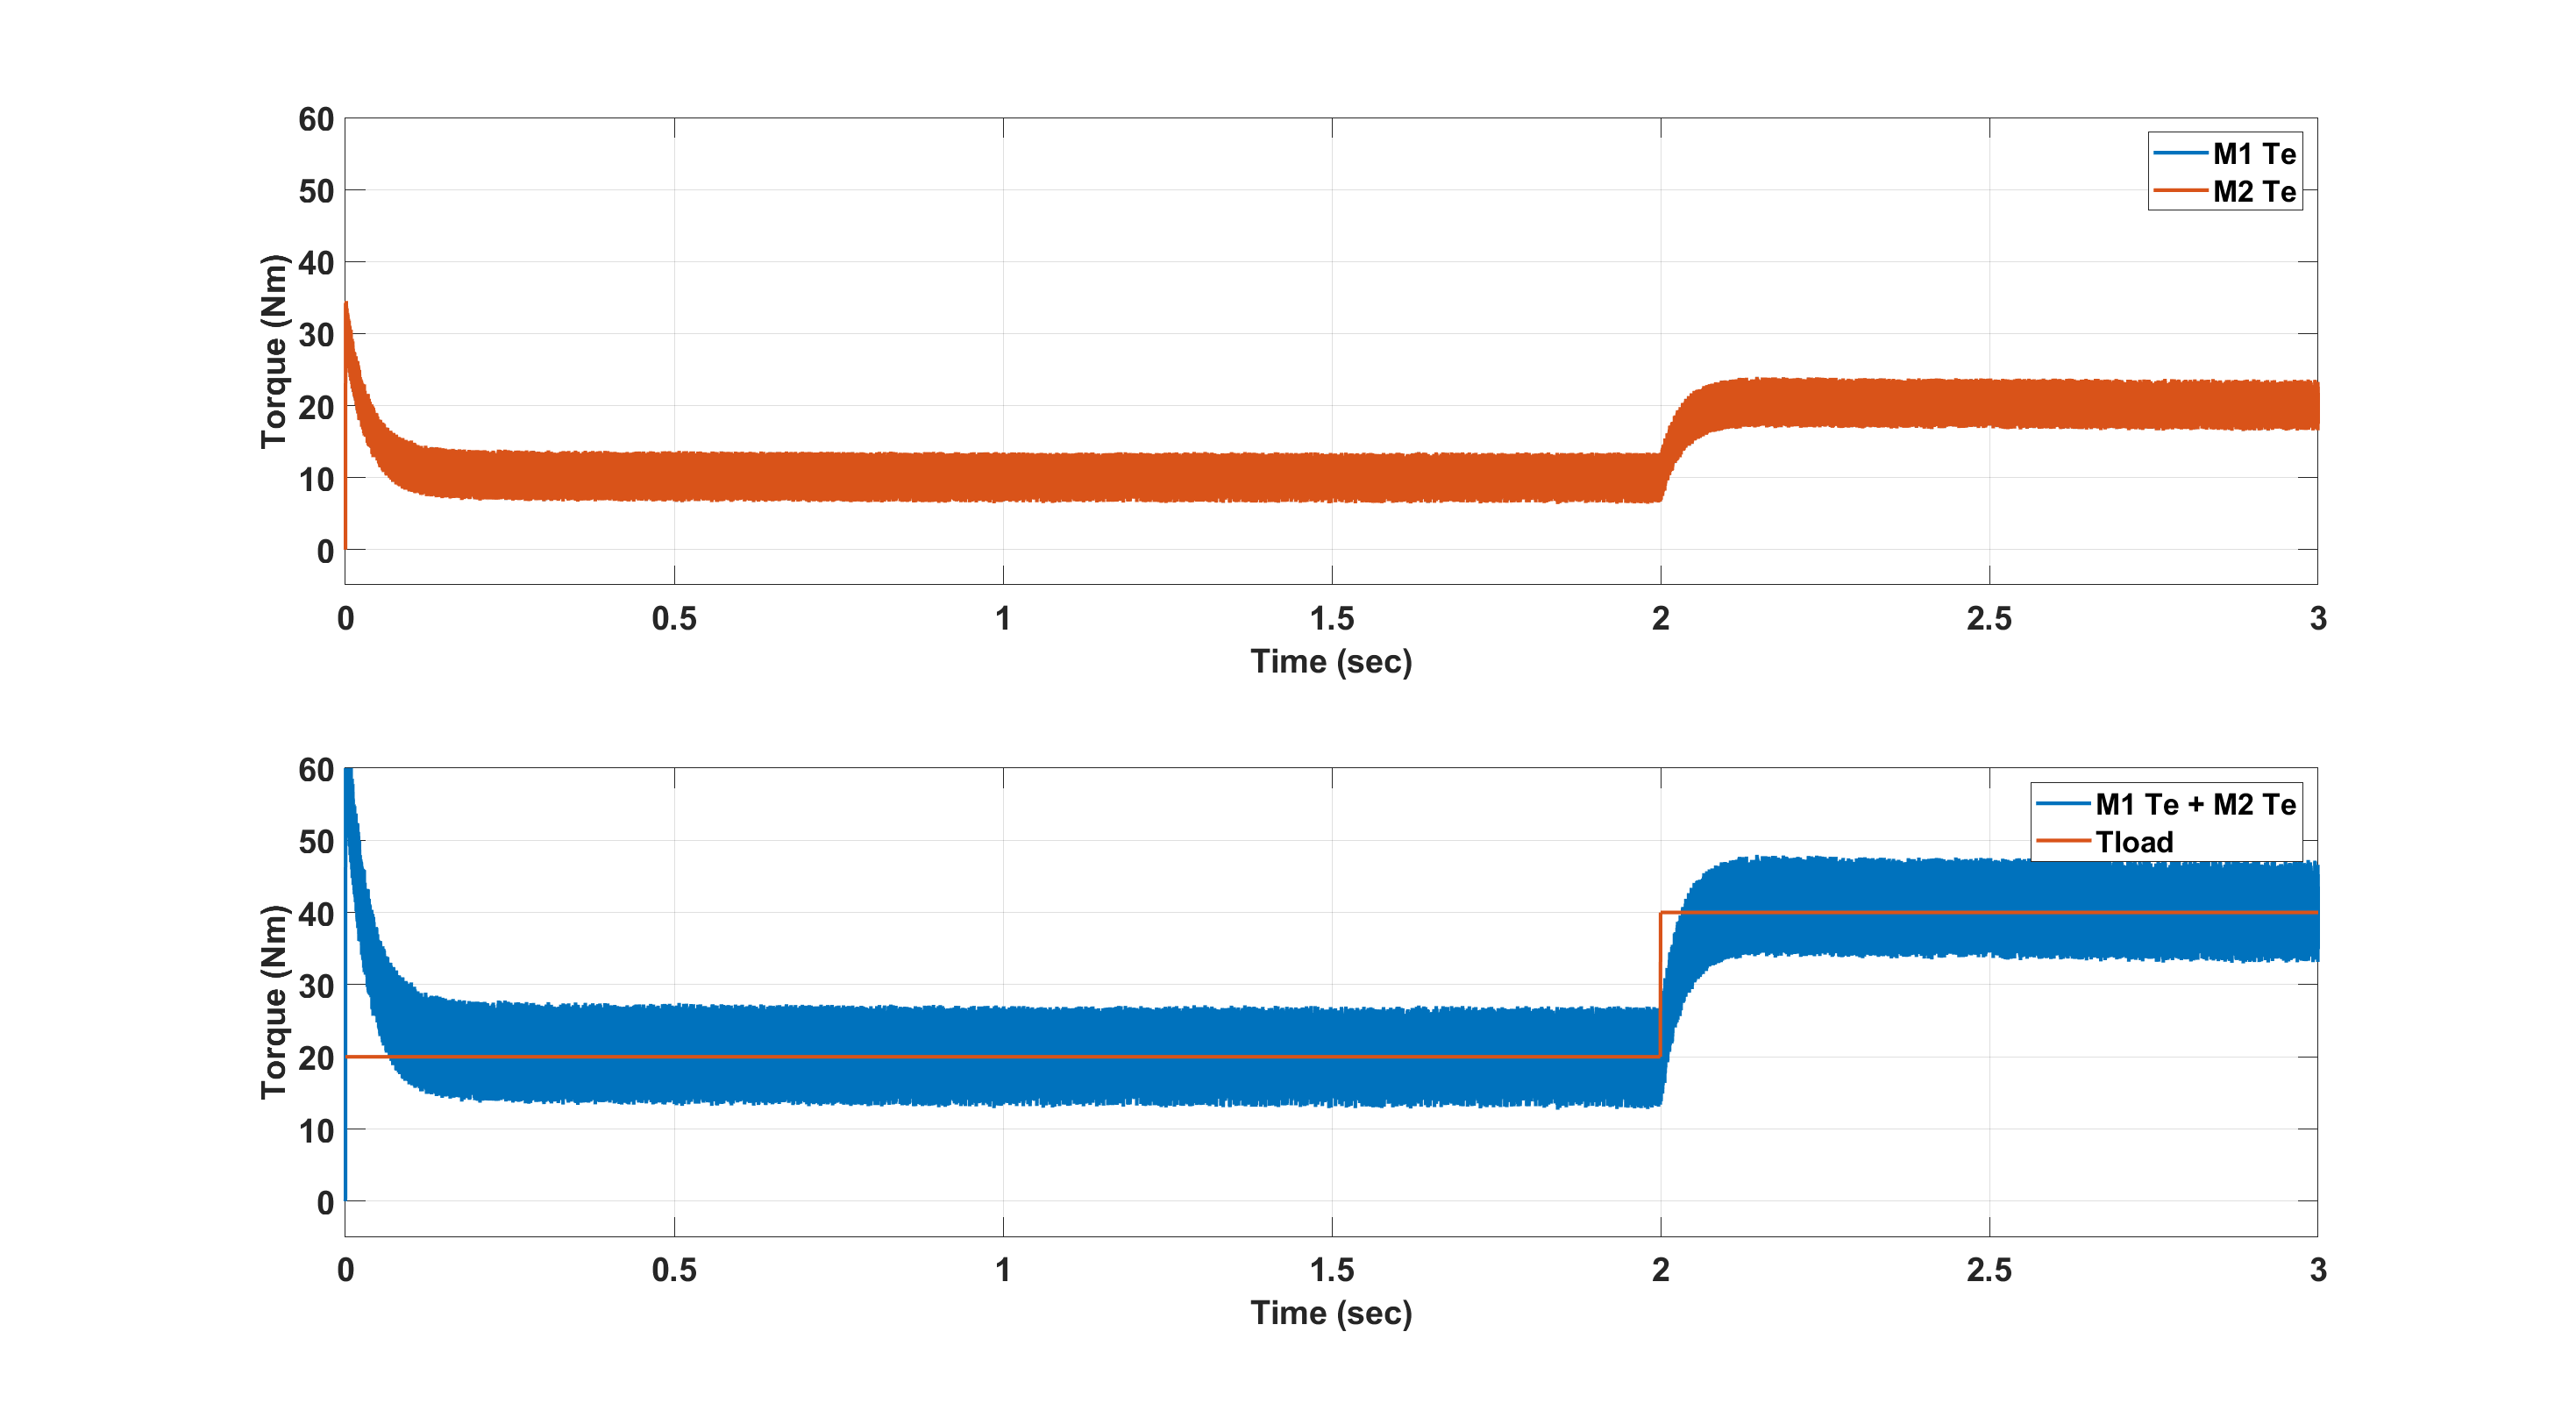
\includegraphics[scale=0.3]{Figures/TwoModule/CombinedCost/Torques.eps}
\caption{Torque generation of each module with combined cost function with no open circuit fault}
\label{fig:Tload_TwoModuleCombinedCost}
\end{figure}
\begin{figure}[H]
\centering
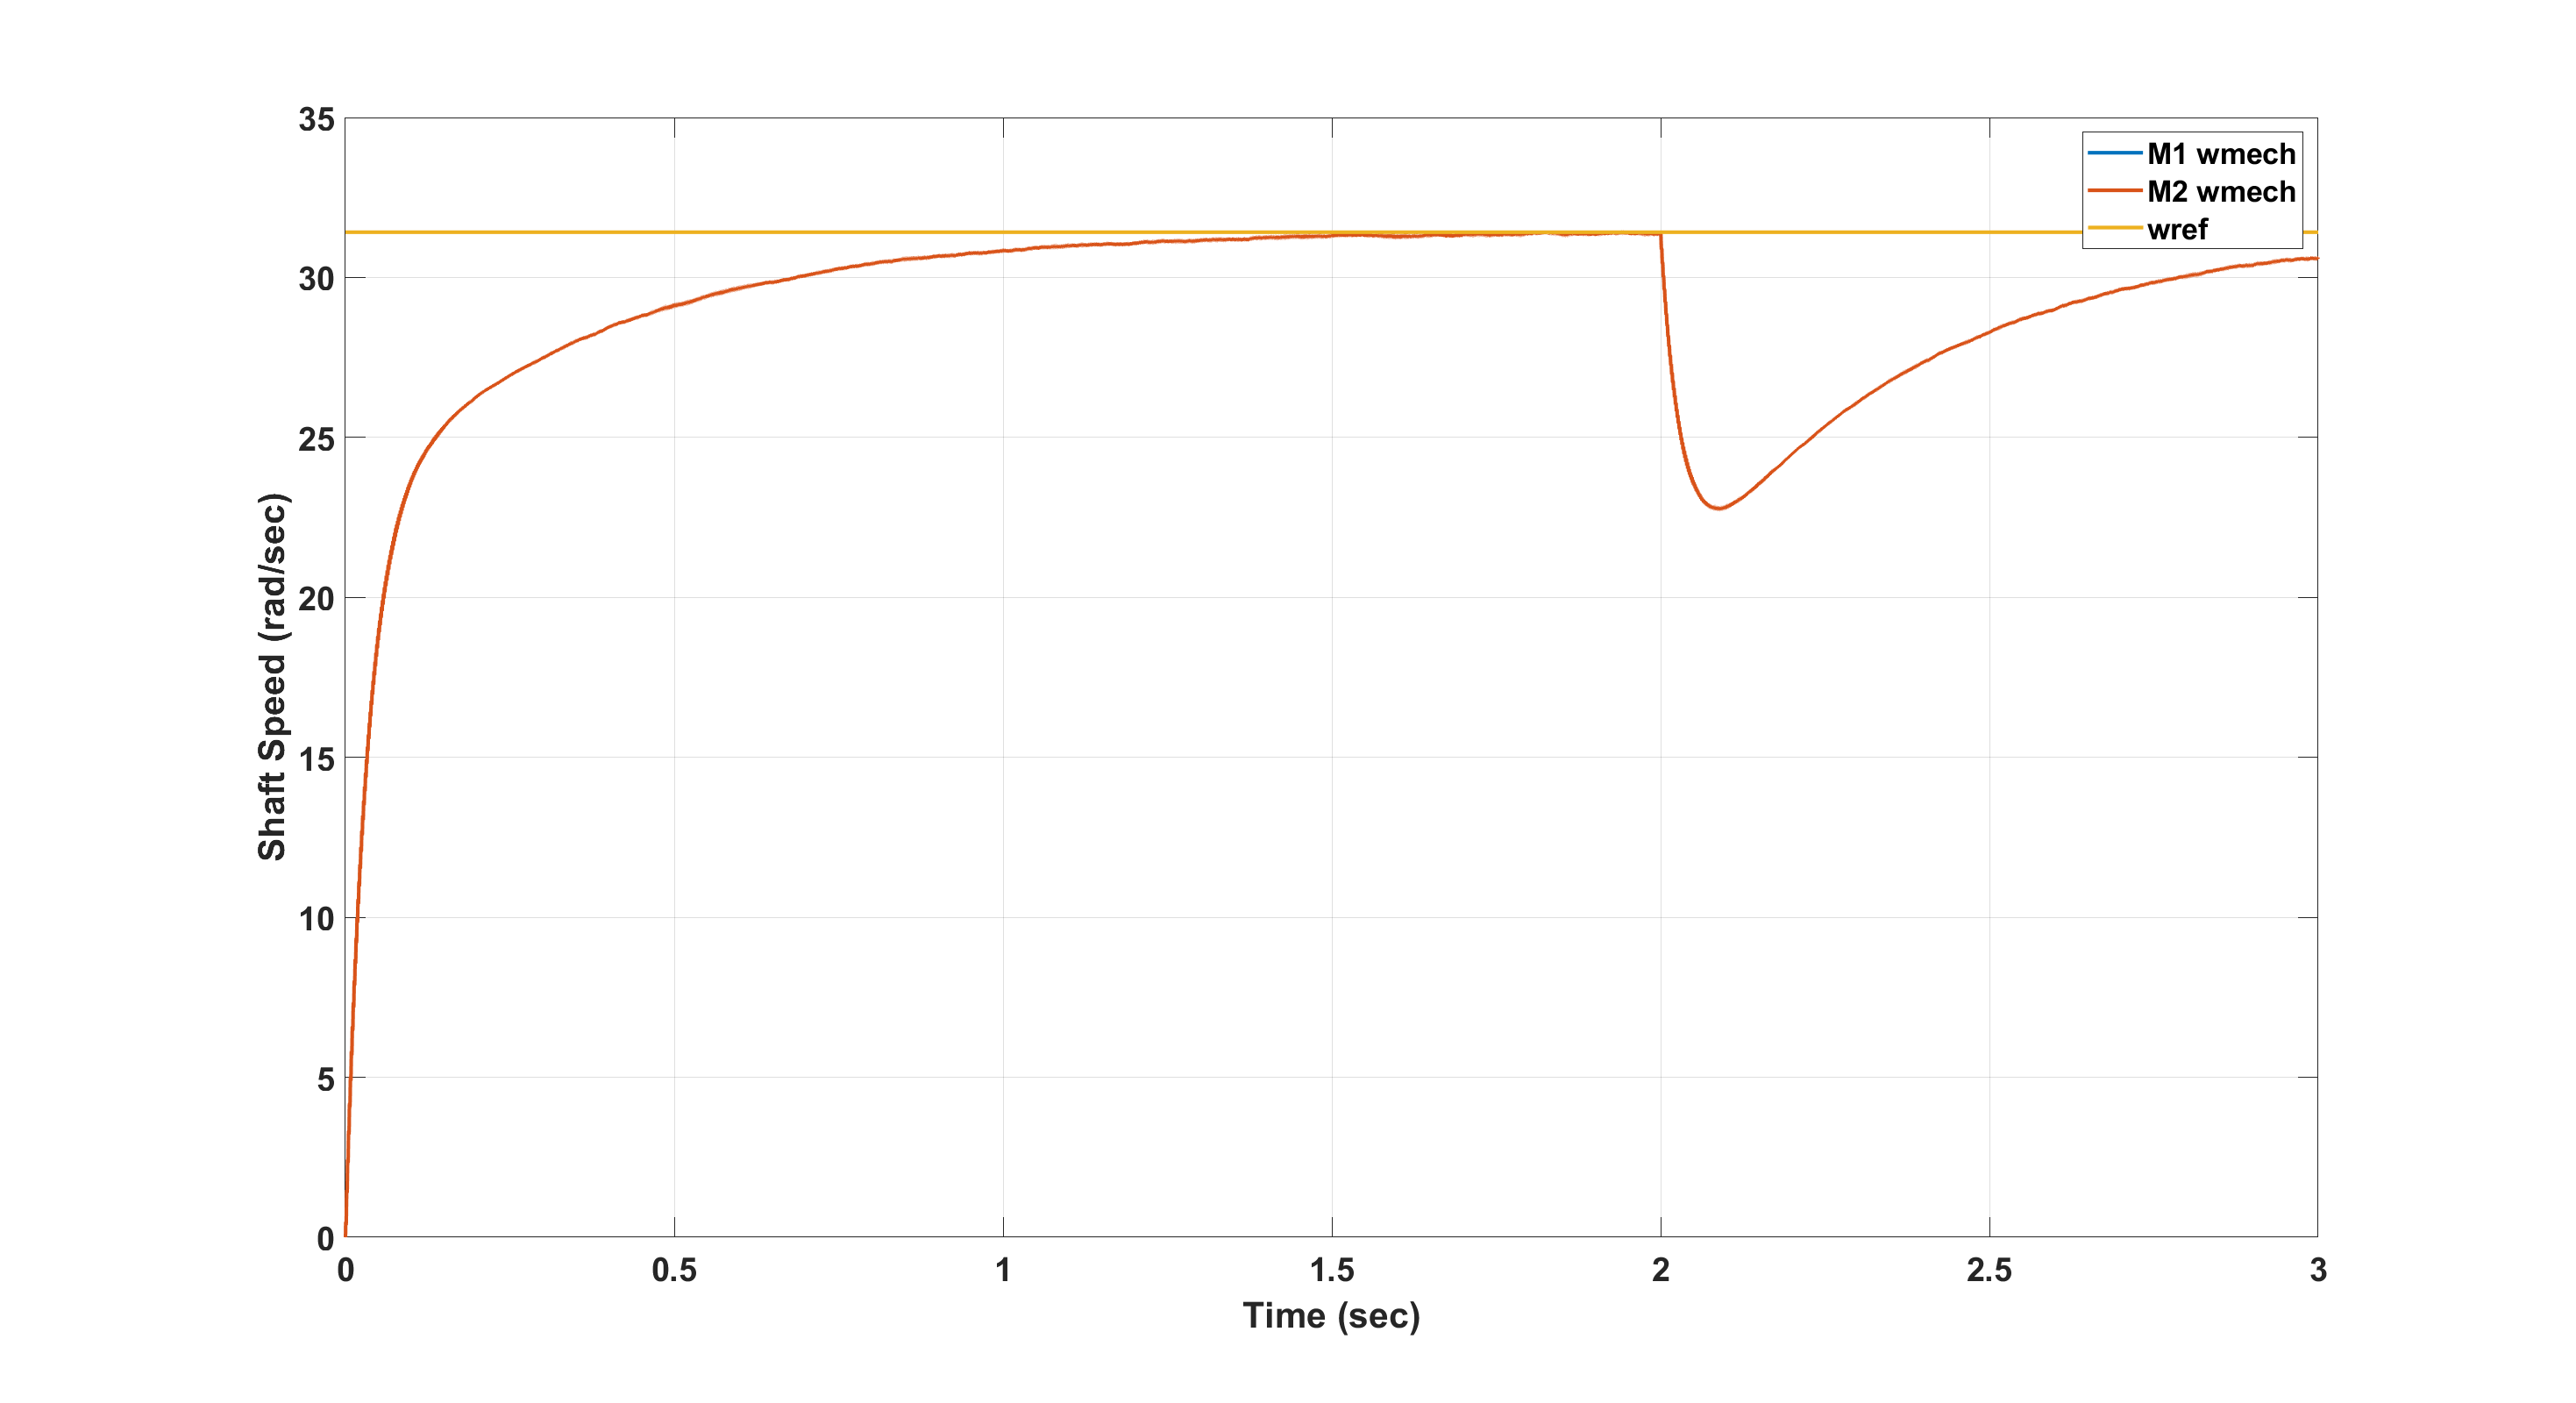
\includegraphics[scale=0.3]{Figures/TwoModule/CombinedCost/ShaftSpeed.eps}
\caption{Shaft speed with combined cost function no open circuit fault}
\label{fig:Wshaft_TwoModuleCombinedCost}
\end{figure}
\begin{figure}[H]
\centering
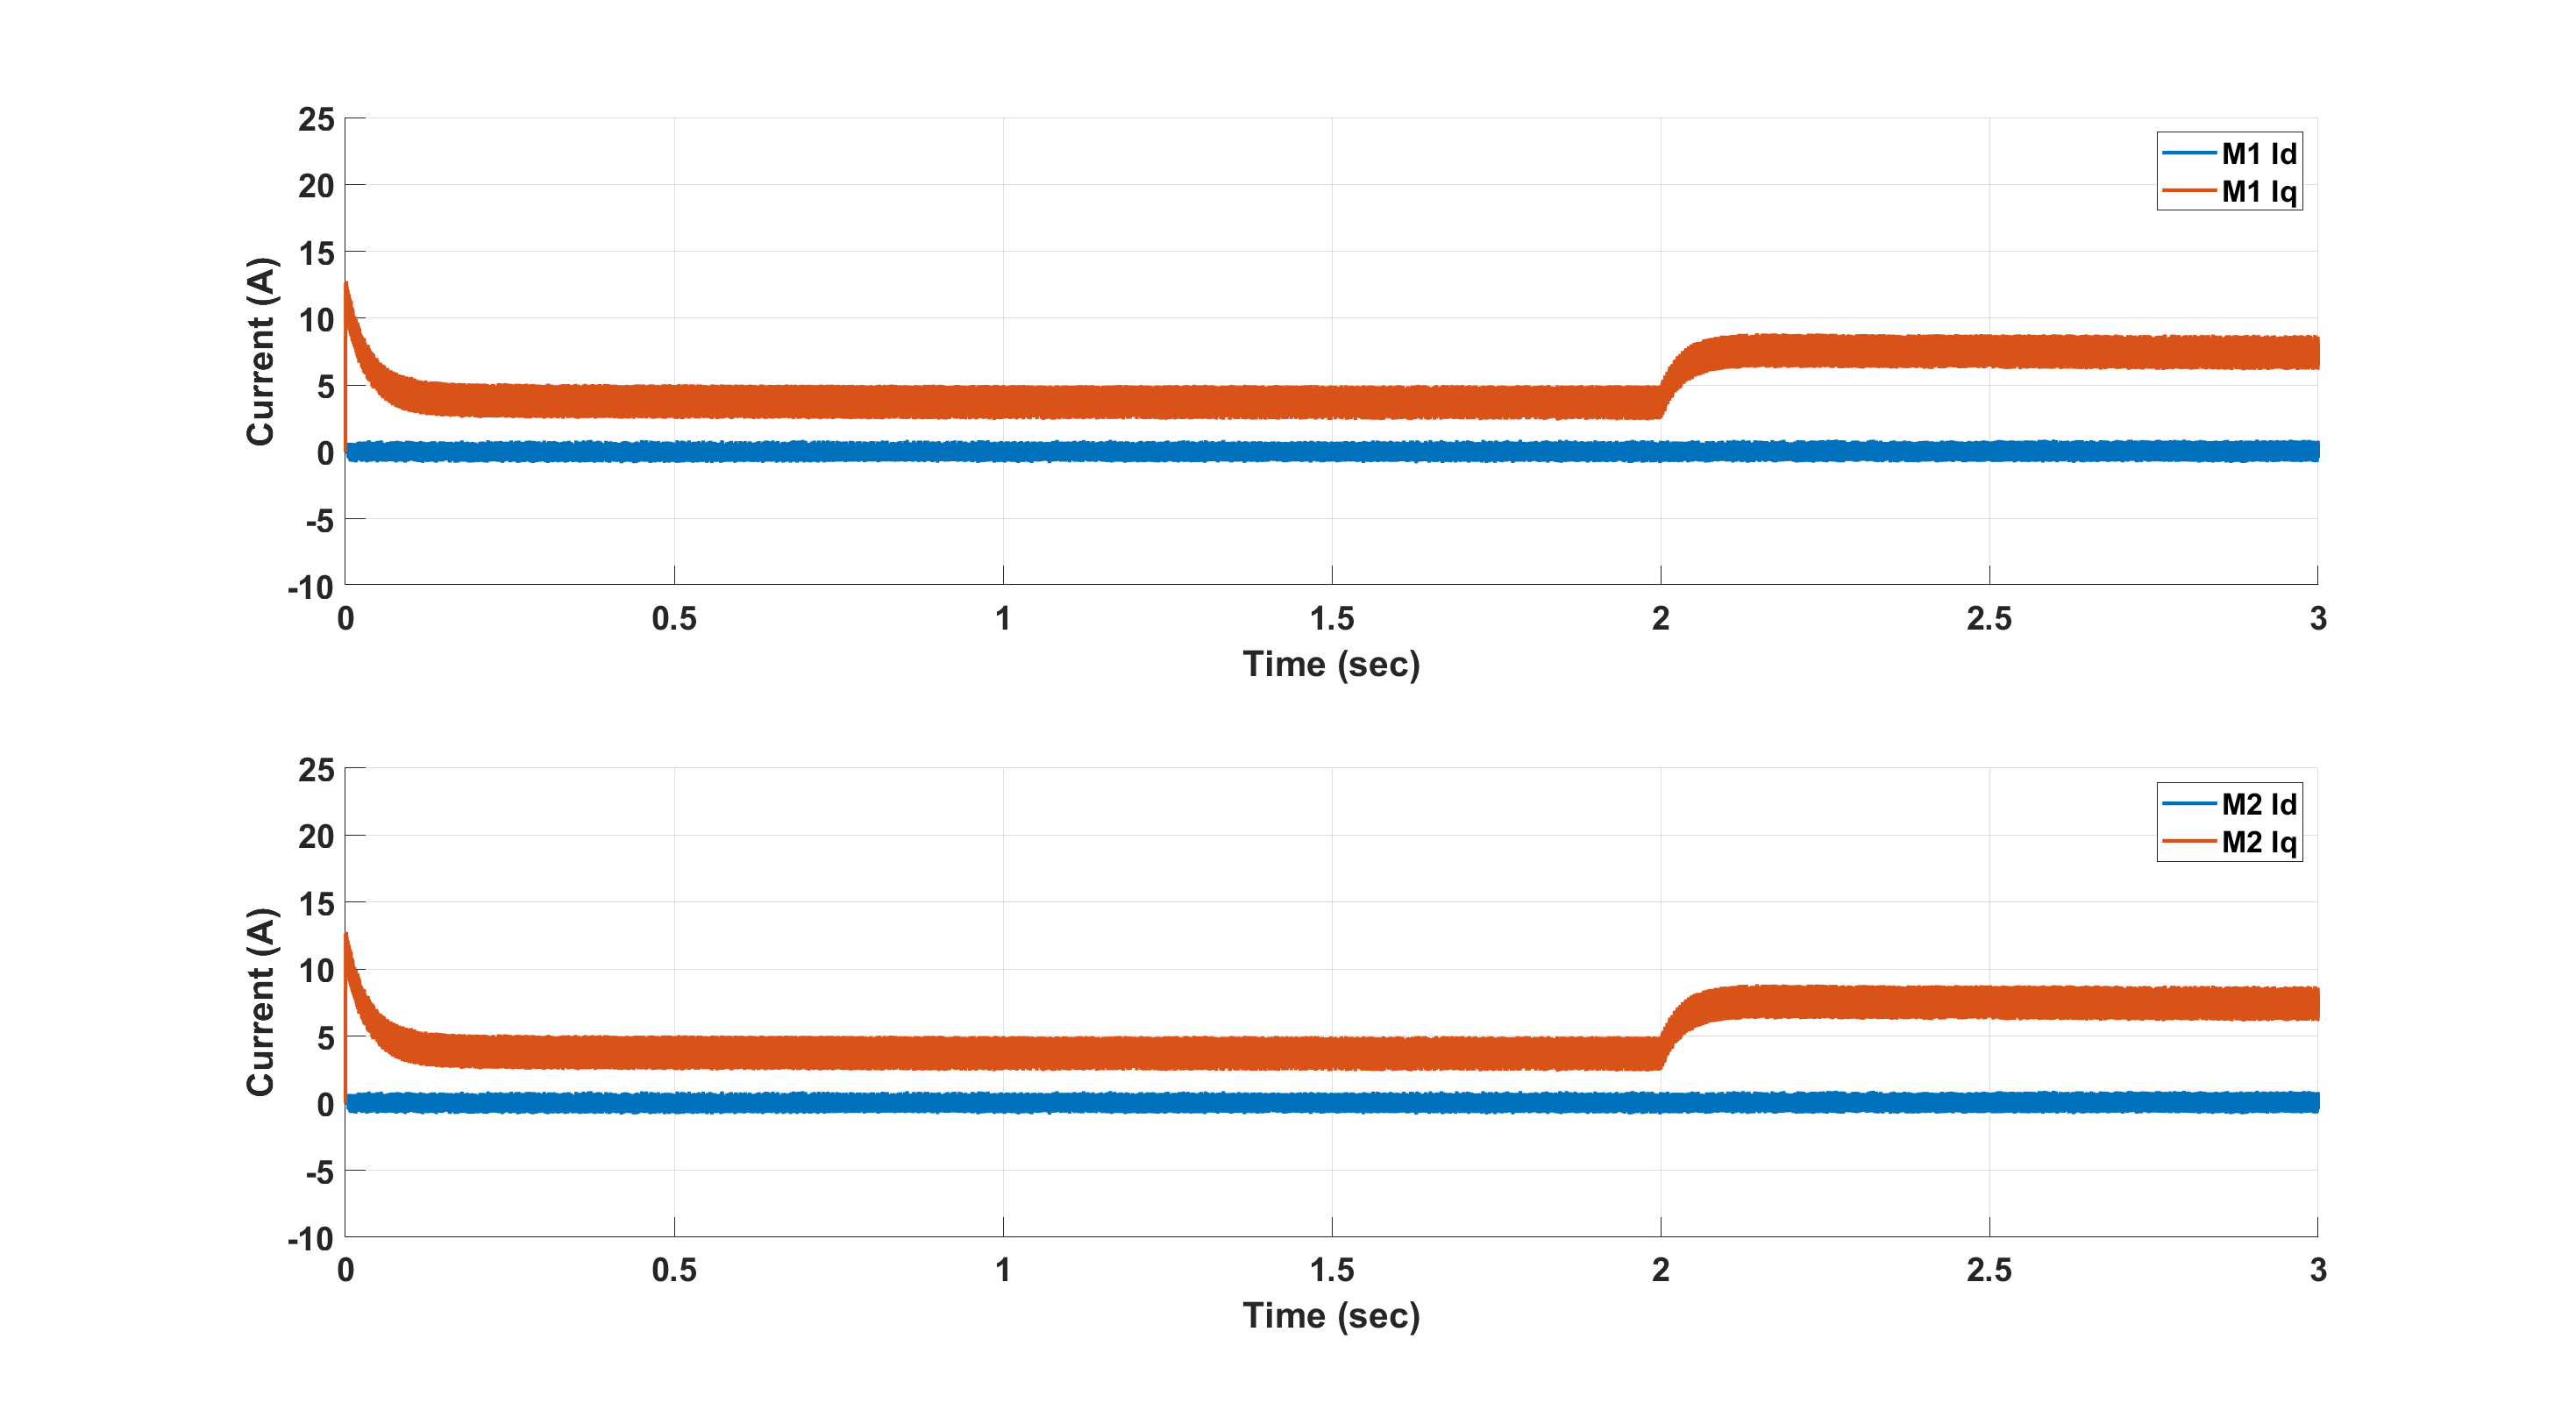
\includegraphics[scale=0.3]{Figures/TwoModule/CombinedCost/Id_Iq.eps}
\caption{Id Iq for Two Modules with combined cost function no open circuit fault}
\label{fig:Current_dq_TwoModuleCombinedCost}
\end{figure}
\begin{figure}[H]
\centering
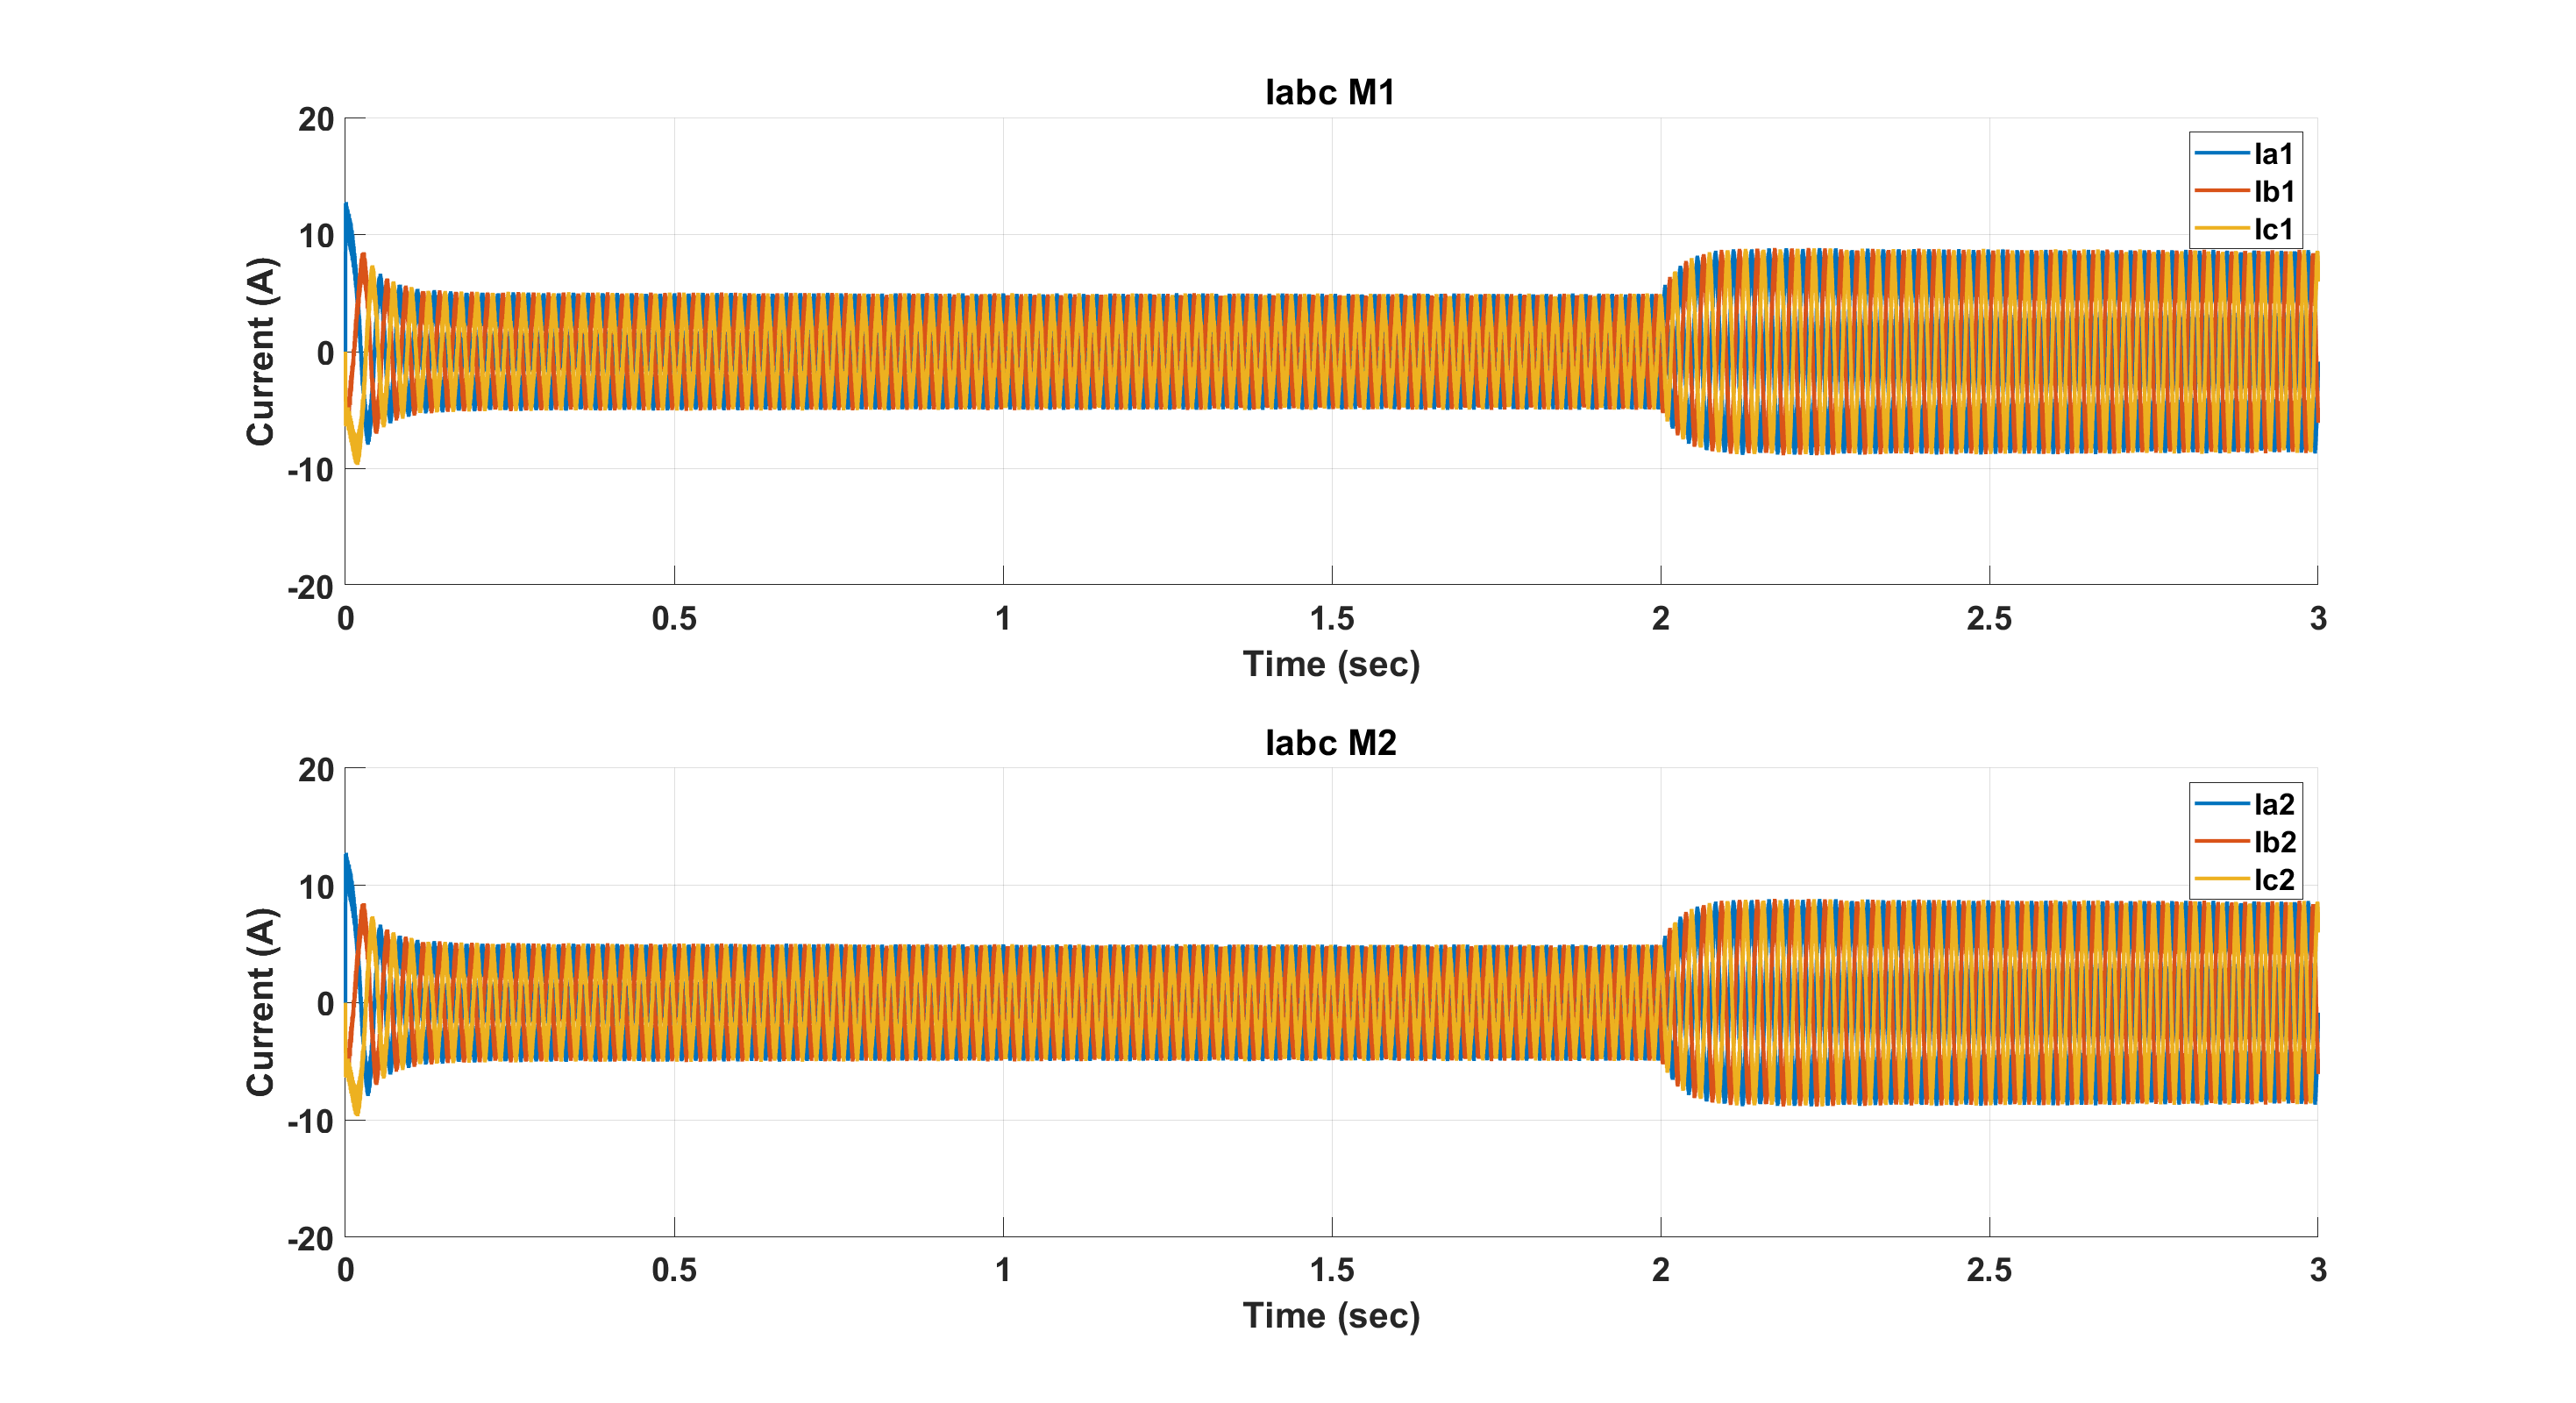
\includegraphics[scale=0.3]{Figures/TwoModule/CombinedCost/Ia_Ib_Ic.eps}
\caption{Phase Currents for Two Modules with combined cost function no open circuit fault}
\label{fig:Current_abc_TwoModuleCombinedCost}
\end{figure}

\subsubsection{Faulty Operation}
In the open circuit operation, the combined cost function method resulted in a more desirable operation. As can be seen in Figure \ref{fig:FaultMomentCombinedCost}. However, in this configuration, the same switching vectors are evaluated for both modules. To be more clear, only 8 switching vectors (same vector for both modules) are evaluted for the combined cost function. The switching vector chosen in this configuration may not be optimum, since all the vector combinations are not evaluted. This is further evaluted in the next section.

\begin{figure}[H]
\centering
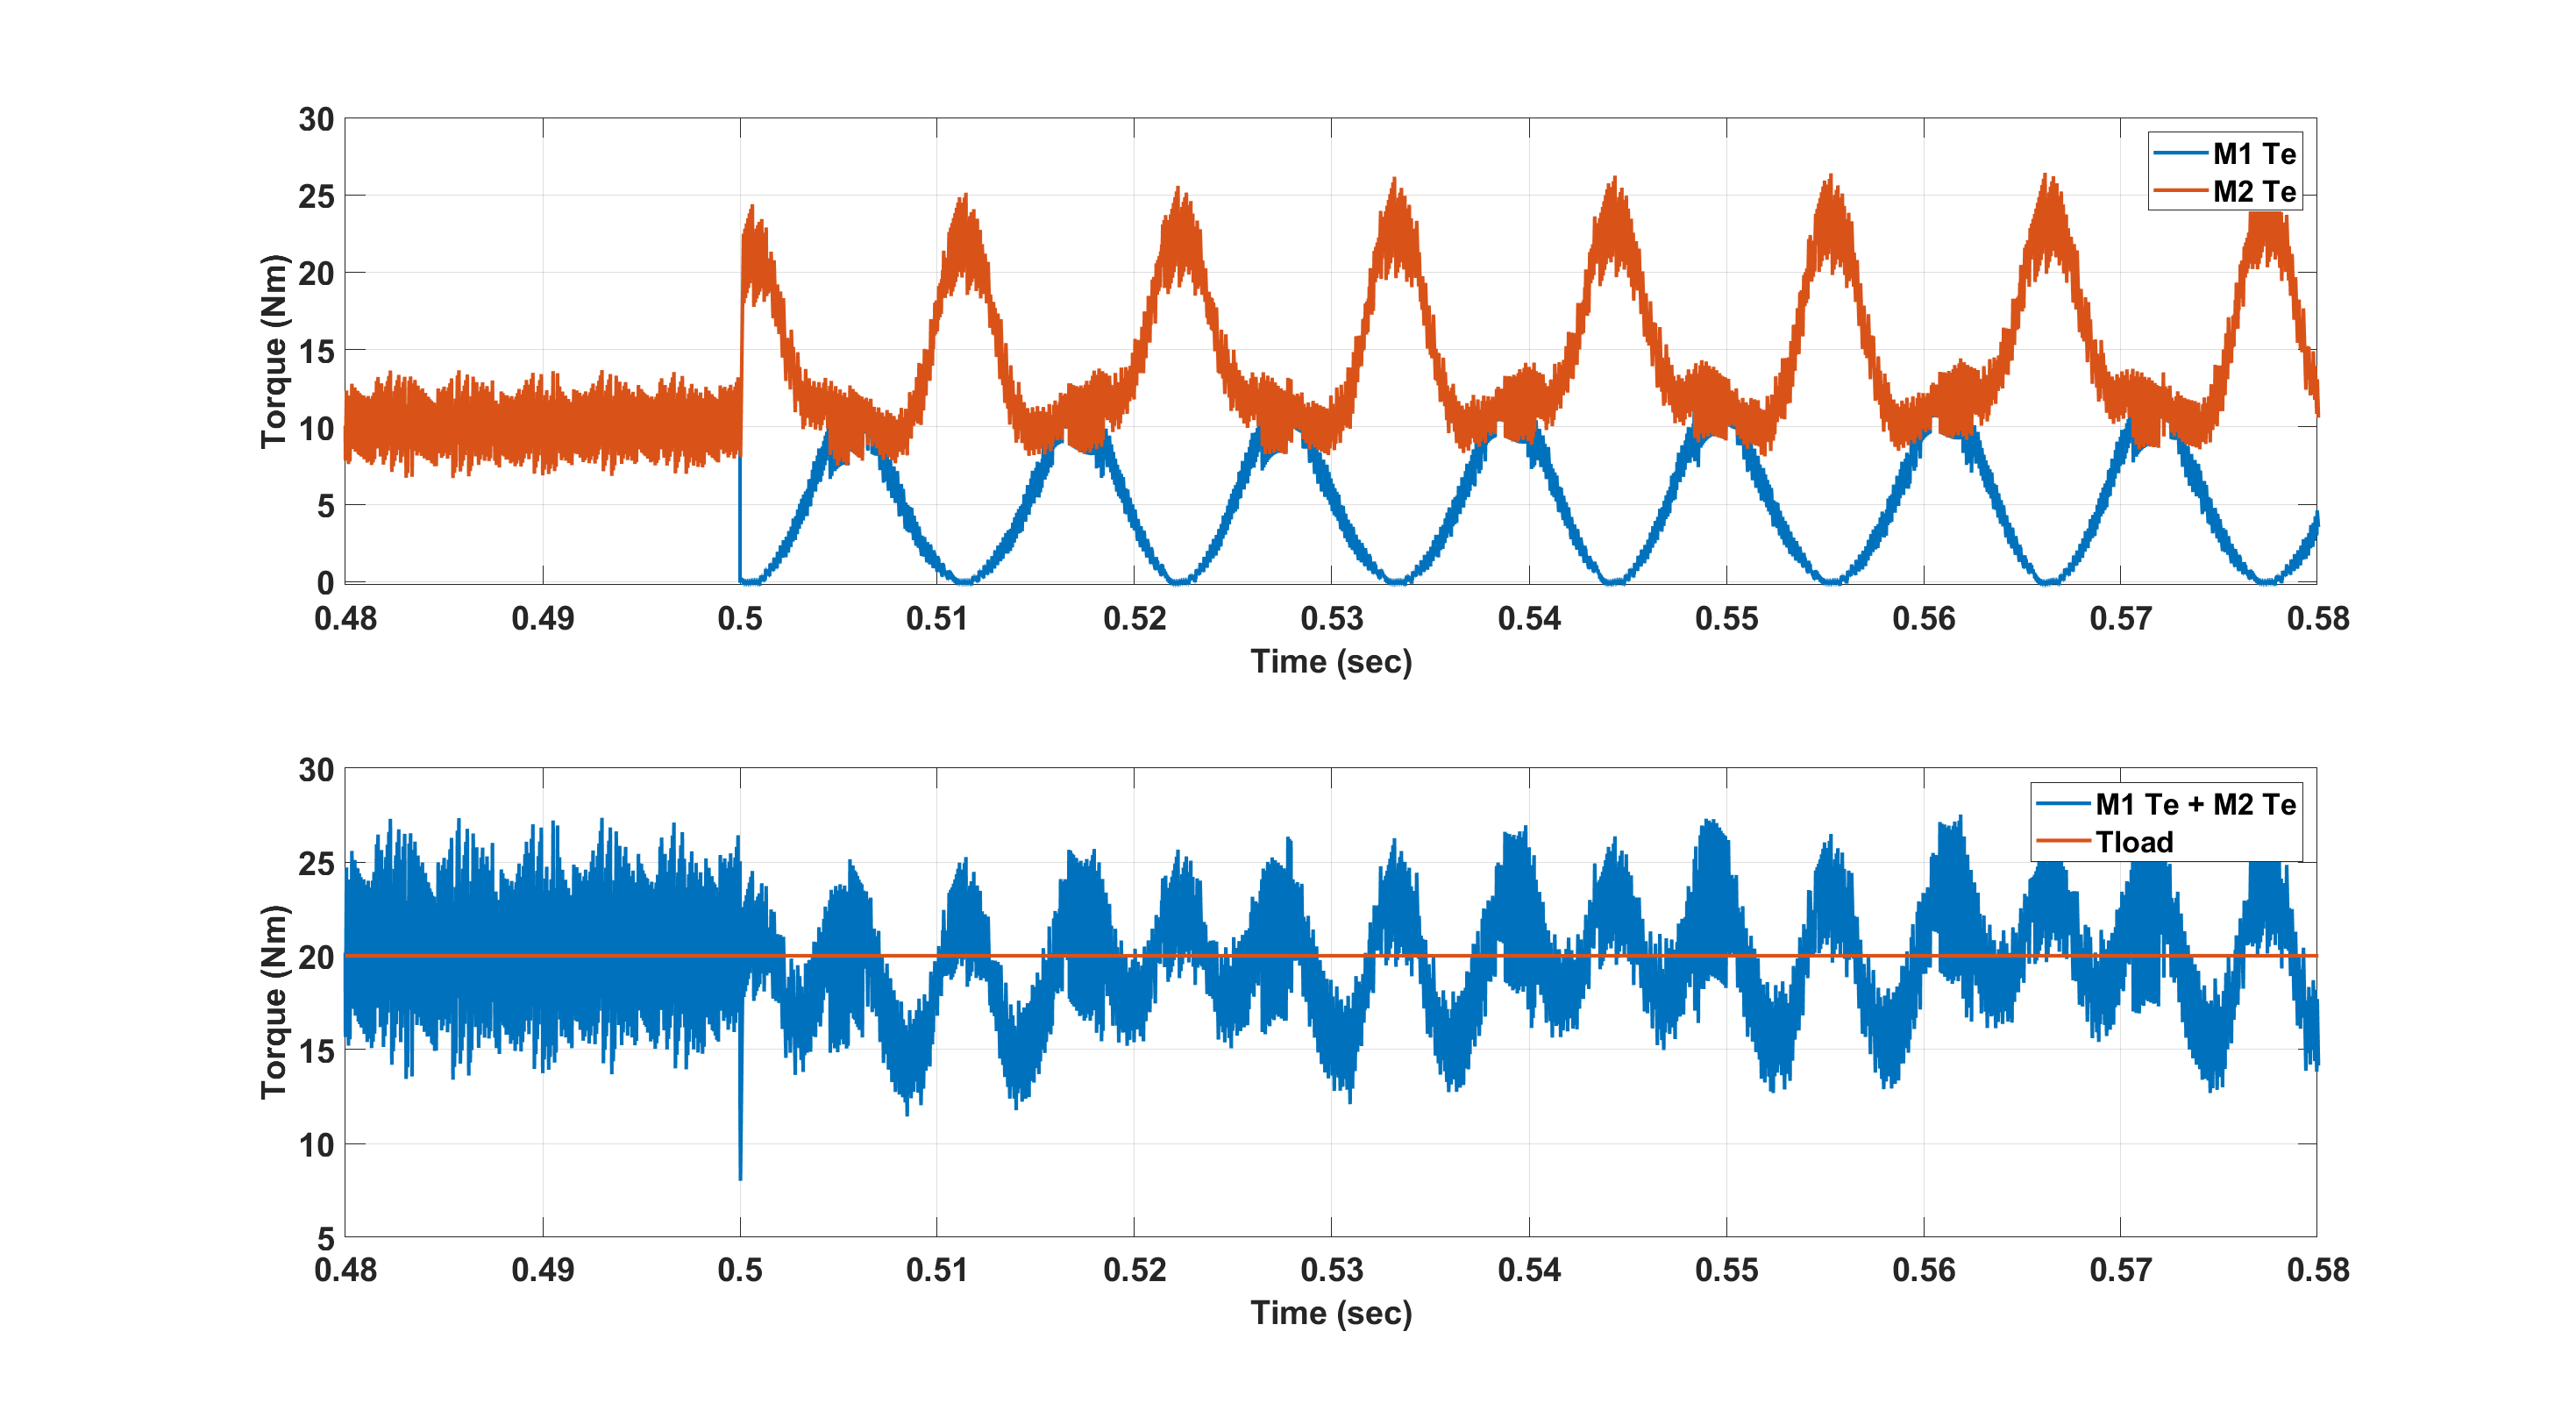
\includegraphics[scale=0.3]{Figures/TwoModule/CombinedCost/FaultMoment.eps}
\caption{Torque Generation at Fault Moment of each module for combined cost function}
\label{fig:FaultMomentCombinedCost}
\end{figure}

\subsection{Combined Cost Function V2, evaluation of every switching vector combinations for two modules}
In this section, the switching vector evaluation for every possible switching combinations (8*8=64) for two modules is provided. This approach can provide the optimum switching vector since all the combinations are evaluated with the cost function. The drawback is that the computational load increases exponentially. 

The total cost function at line \ref{line:Two_Module_cost_combined_V2} of listings \ref{code:TwoModuleCombinedCostV2}. There two for loops for evaluating to evaluate every switching combinations.

\subsubsection{Healthy Operation}
\label{section:HealthyTwoModuleCombinedV2}
The simulation results for Healthy operation for combined cost function is provided in Figures \ref{fig:Tload_TwoModuleCombinedCostV2}, \ref{fig:Wshaft_TwoModuleCombinedCostV2}, \ref{fig:Current_dq_TwoModuleCombinedCostV2}, \ref{fig:Current_abc_TwoModuleCombinedCostV2}. In the cost function, the following parameters evaluated (as can be seen in line \ref{line:Two_Module_cost_combined_V2} of listing \ref{code:TwoModuleCombinedCostV2}).
\begin{itemize}
    \item Torque error
    \item Module 1 Id current
    \item Module 2 Id current
    \item Torque and current limits.
\end{itemize}
In the healthy operation simulations, it can be seen that the combined torque generated seem to be not different from other simulations (Figure \ref{fig:Tload_TwoModuleCombinedCostV2}). However, individual current and torque values of the modules seem to have a high ripples. In my opinion there needs to be an extra constraint for the selection of switching vectors. "Lack of constraints cause freedom of choice of switching vectors, which is not optimum", see Section \ref{section:FaultyTwoModuleCombinedV2}.
At first, I tried to make the modules to share the same torque value. However, under the faulty condition, the healthy modules started to produce the same torque as the faulty module, their torque ripples are added up, which is not desired. Therefore I concluded that there needs to be an extra constraint on the cost function evalution such as minimizing the conduction loss for both modules. 

\begin{figure}[H]
\centering
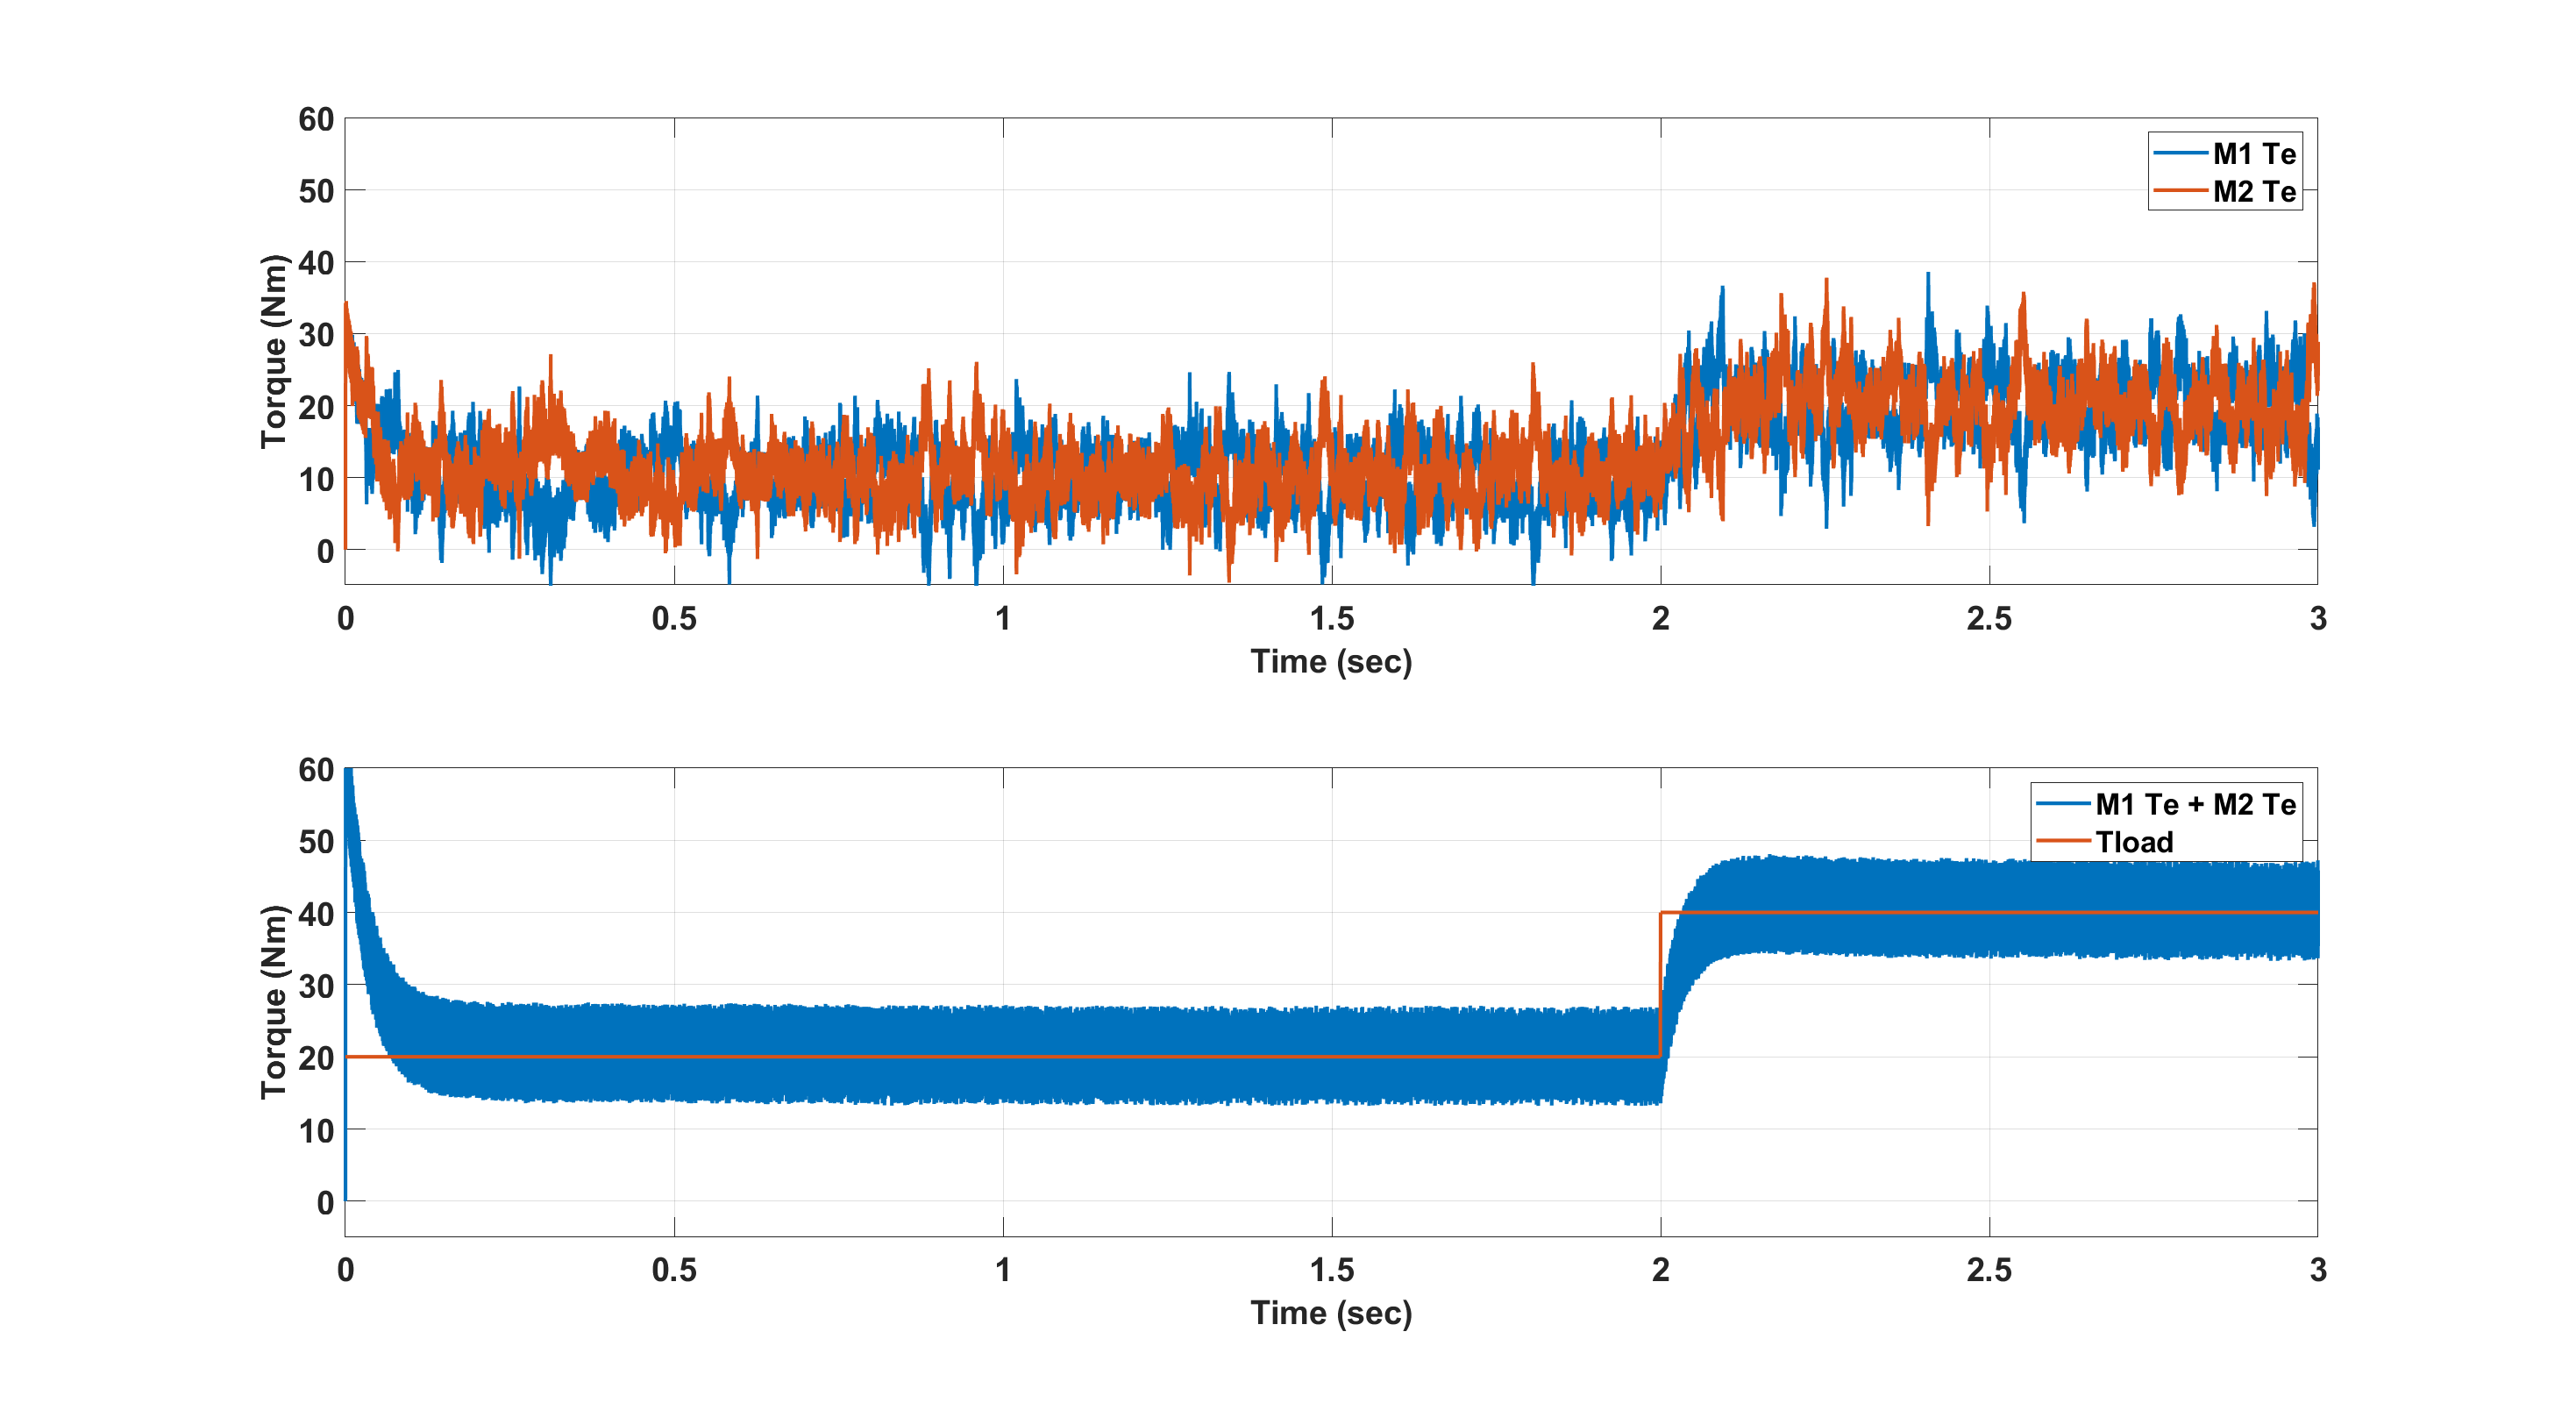
\includegraphics[scale=0.3]{Figures/TwoModule/CombinedCostV2/Torques.eps}
\caption{Torque generation of each module with combined cost function V2 with no open circuit fault}
\label{fig:Tload_TwoModuleCombinedCostV2}
\end{figure}
\begin{figure}[H]
\centering
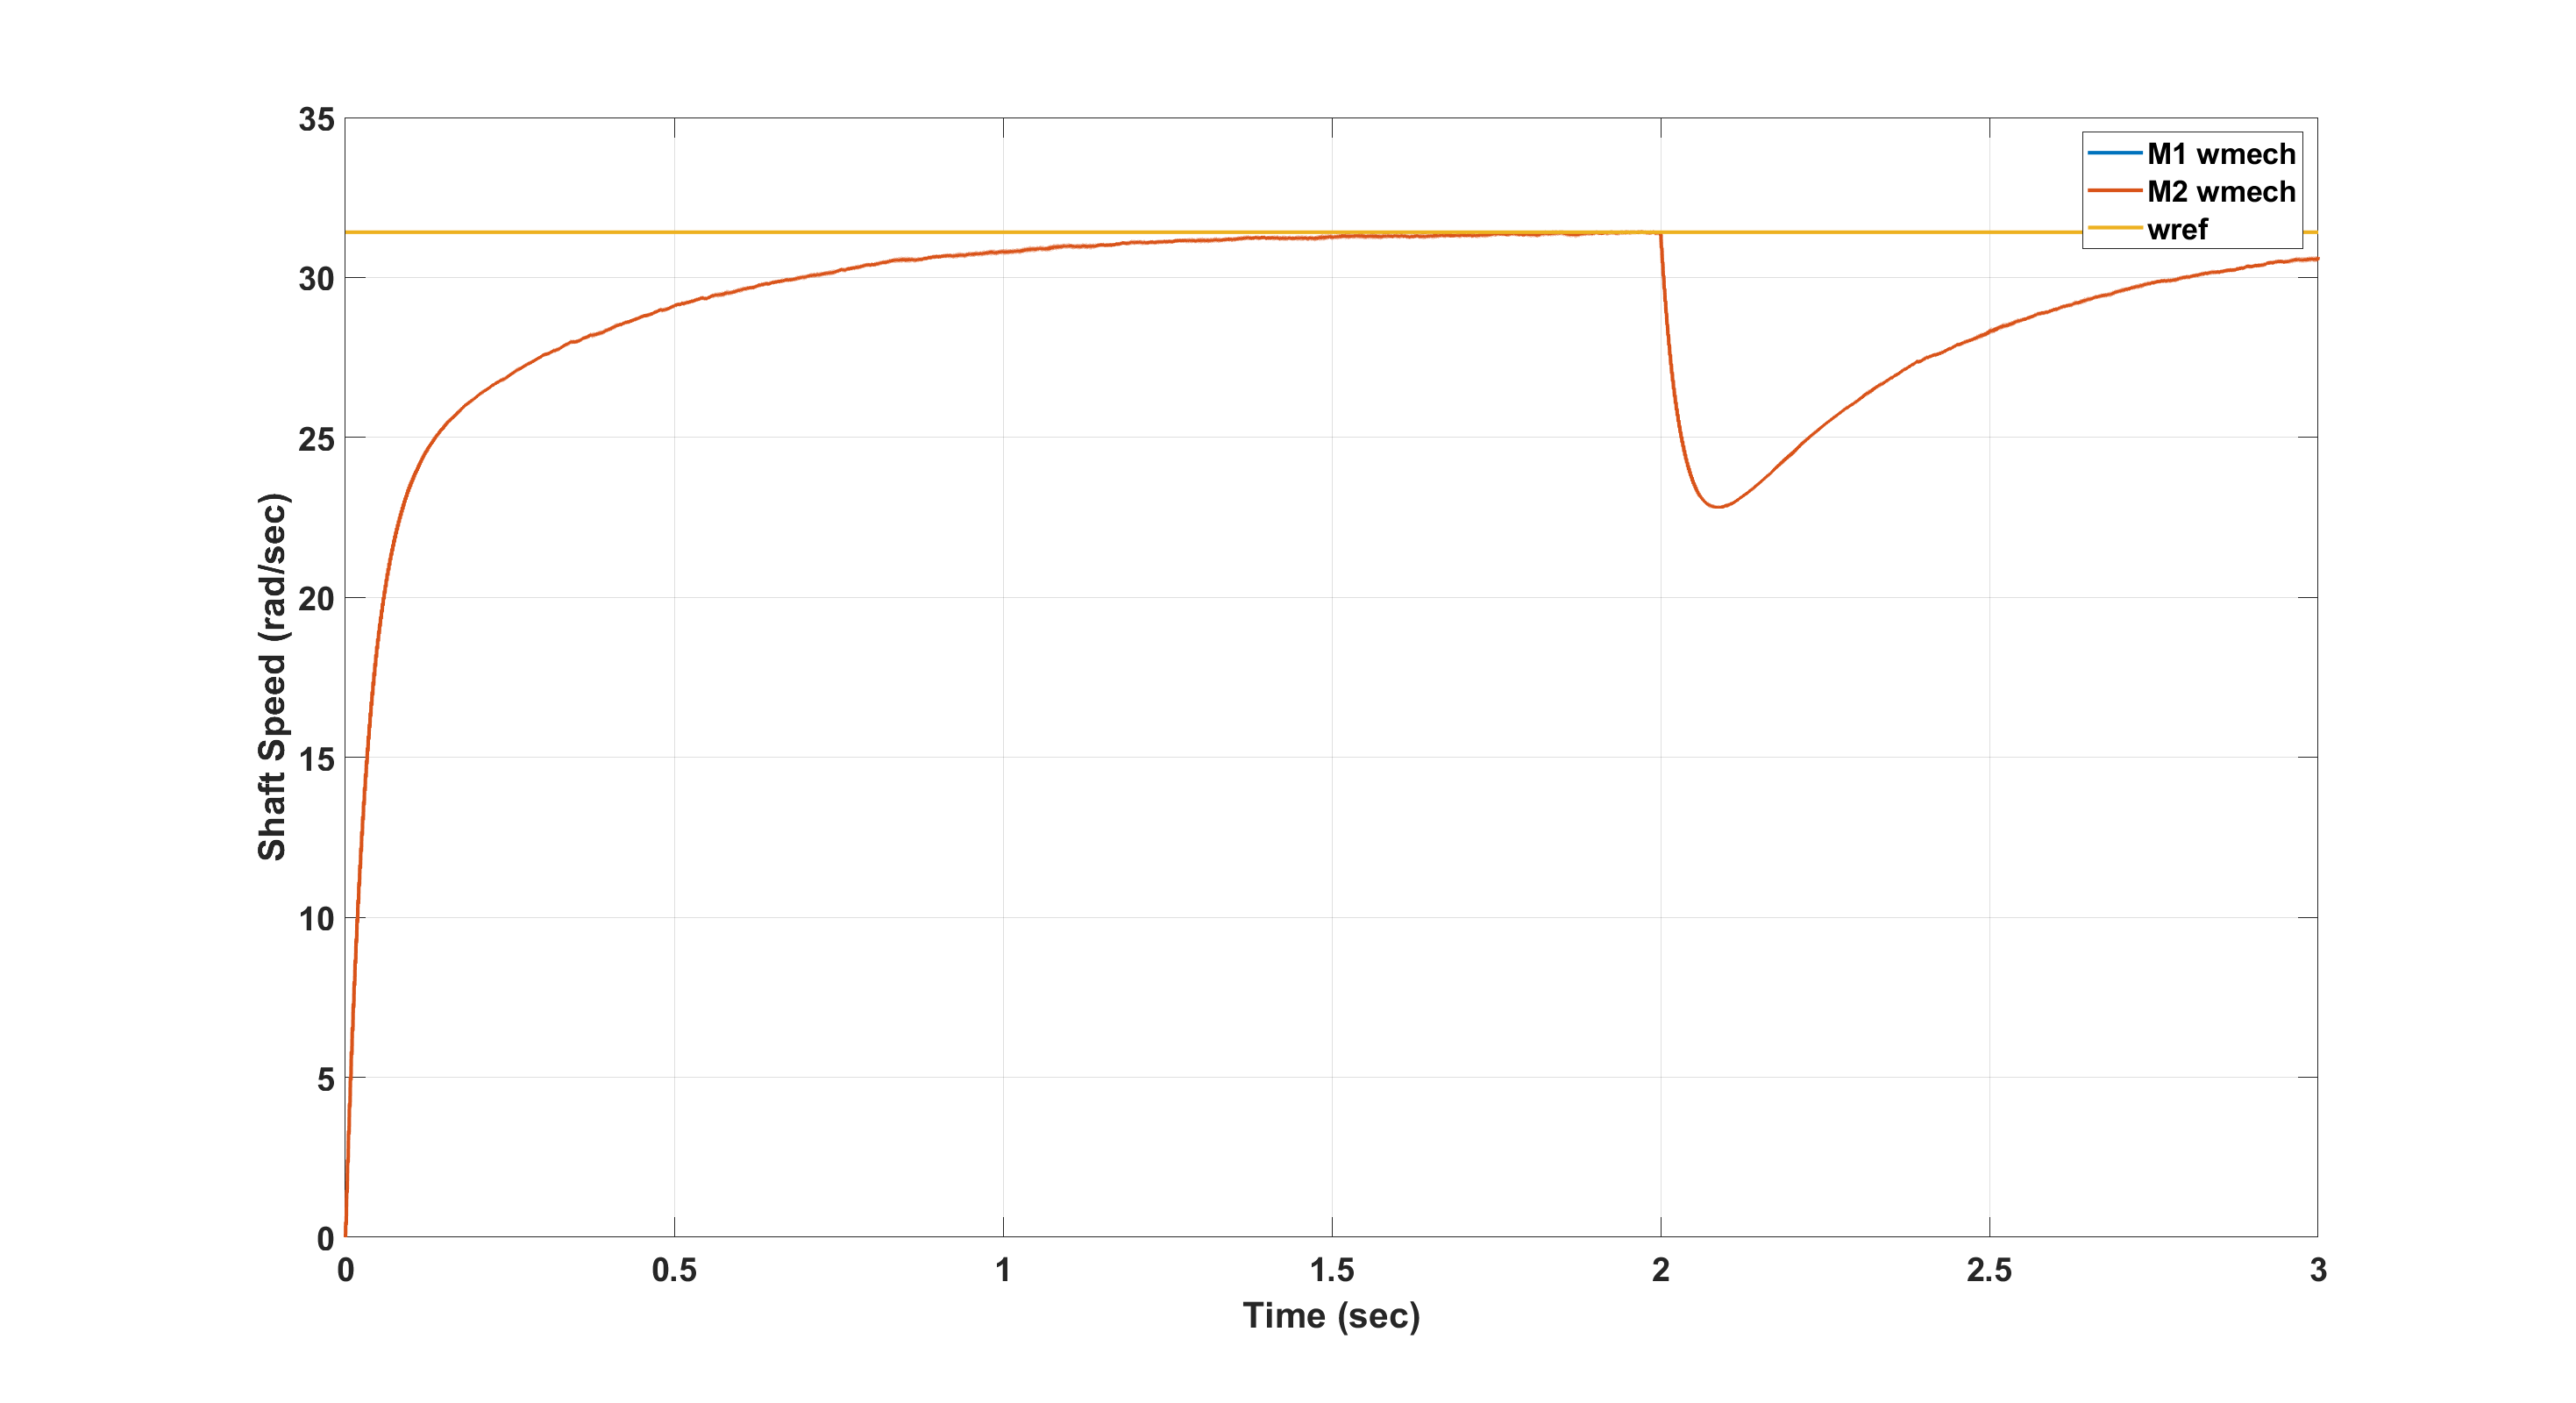
\includegraphics[scale=0.3]{Figures/TwoModule/CombinedCostV2/ShaftSpeed.eps}
\caption{Shaft speed with combined cost function V2 no open circuit fault}
\label{fig:Wshaft_TwoModuleCombinedCostV2}
\end{figure}
\begin{figure}[H]
\centering
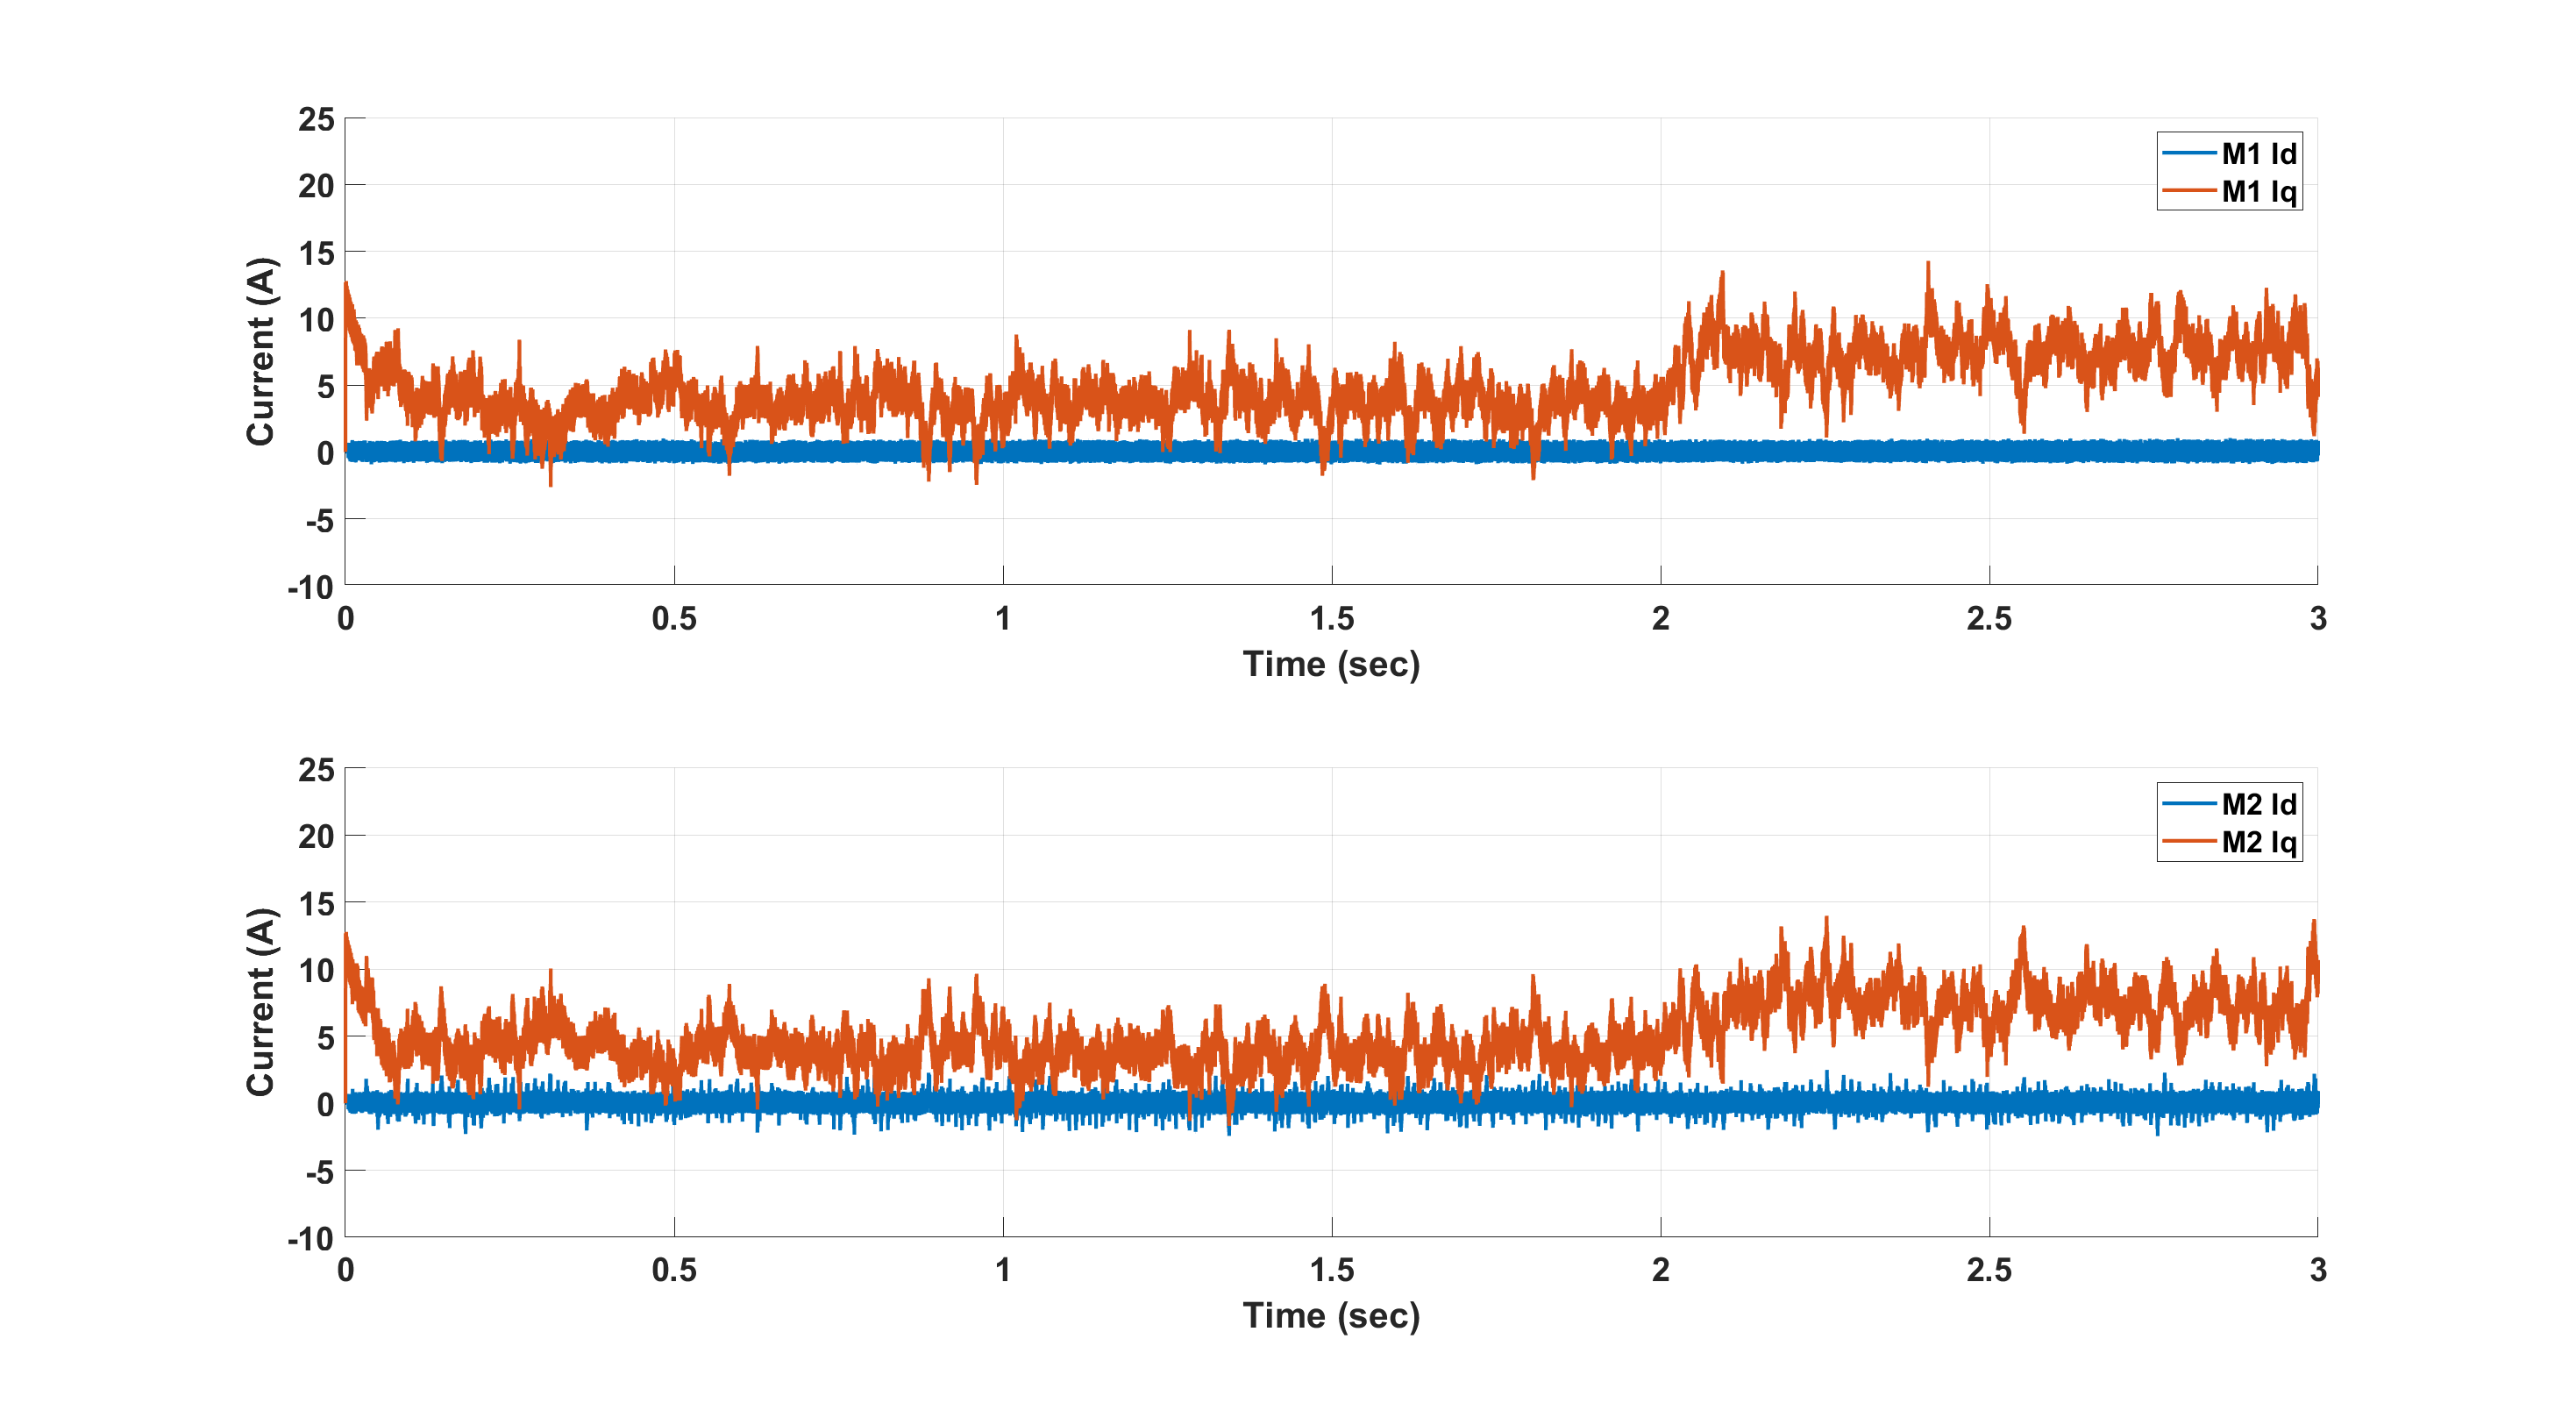
\includegraphics[scale=0.3]{Figures/TwoModule/CombinedCostV2/Id_Iq.eps}
\caption{Id Iq for Two Modules with combined cost function V2 no open circuit fault}
\label{fig:Current_dq_TwoModuleCombinedCostV2}
\end{figure}
\begin{figure}[H]
\centering
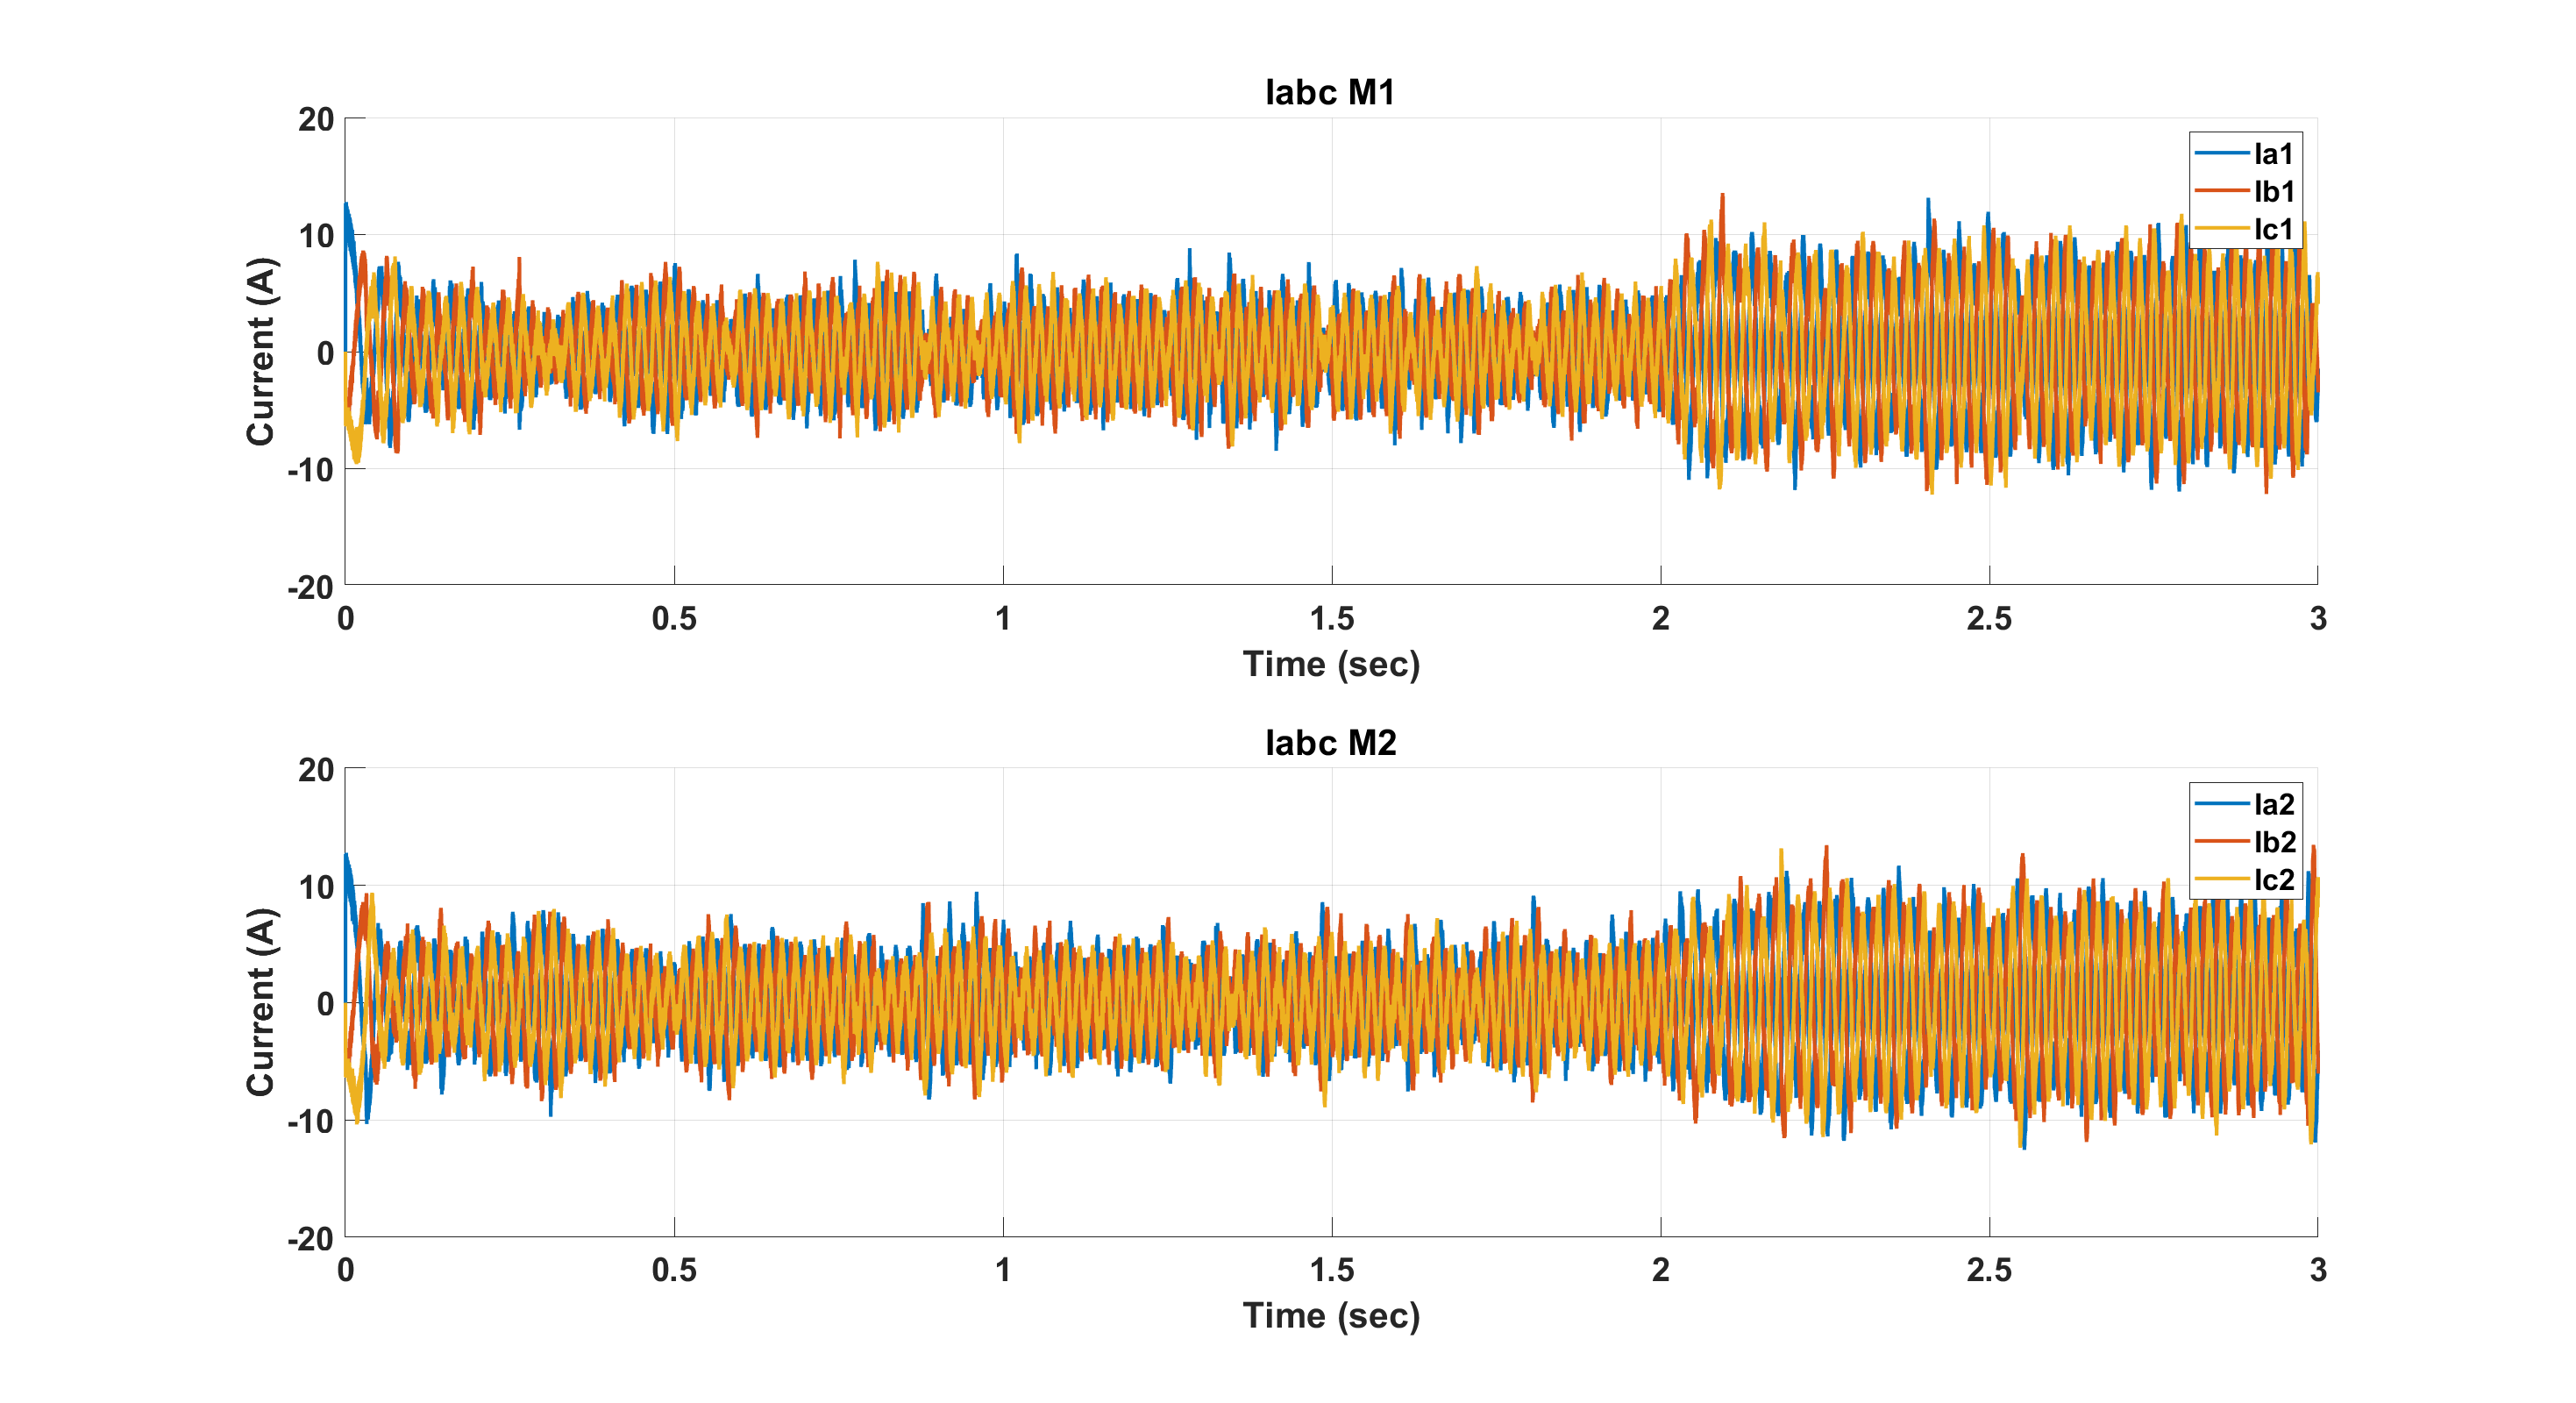
\includegraphics[scale=0.3]{Figures/TwoModule/CombinedCostV2/Ia_Ib_Ic.eps}
\caption{Phase Currents for Two Modules with combined cost function V2 no open circuit fault}
\label{fig:Current_abc_TwoModuleCombinedCostV2}
\end{figure}

\subsubsection{Faulty Operation}
\label{section:FaultyTwoModuleCombinedV2}
The problem of freedom of switching vector choice that is mentioned in \ref{section:HealthyTwoModuleCombinedV2} causes more drastic problem under fault condition. As can be seen in Figure \ref{fig:FaultMomentCombinedCostV2}, even though the combined torque of the system is not absurd, the individual torque generated by each module gets absurd values. 

\begin{figure}[H]
\centering
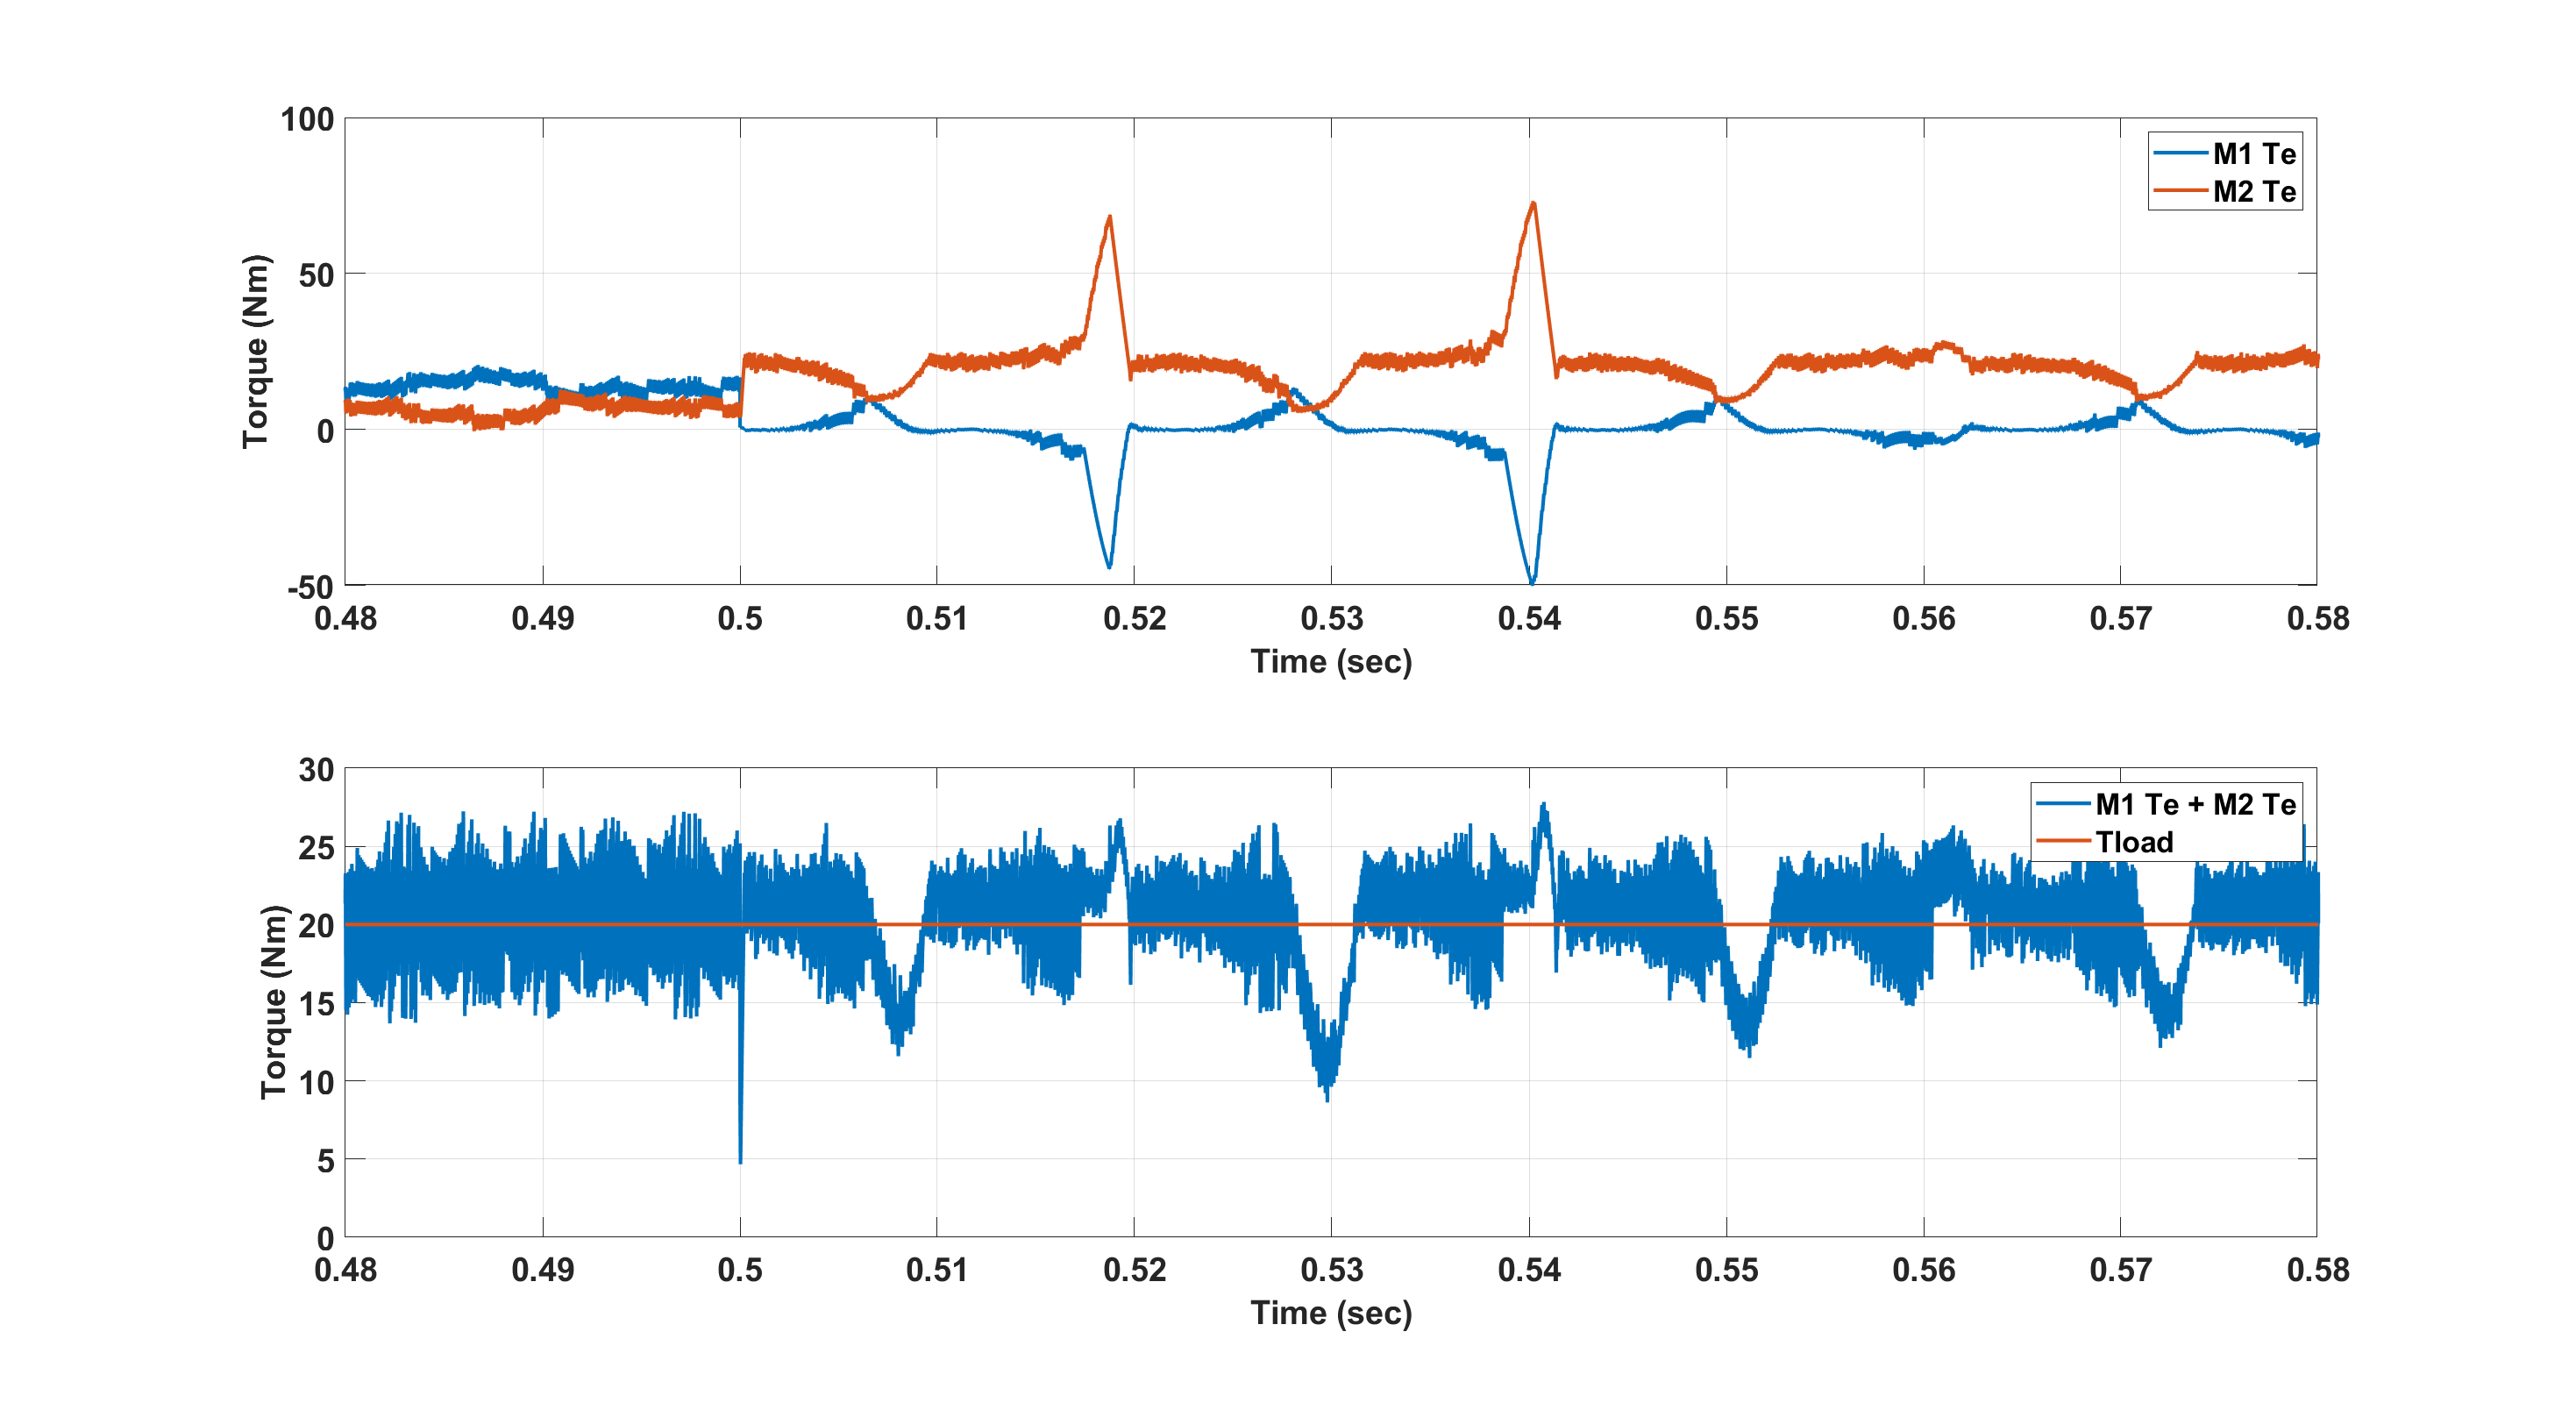
\includegraphics[scale=0.3]{Figures/TwoModule/CombinedCostV2/FaultMoment.eps}
\caption{Torque Generation at Fault Moment of each module for combined cost function V2}
\label{fig:FaultMomentCombinedCostV2}
\end{figure}

\section{Conclusion}
As I have stated in \ref{section:HealthyTwoModuleCombinedV2} and \ref{section:FaultyTwoModuleCombinedV2}, there needs to be extra constaint on the choice of an optimum vector choice. After this point, I am planning to add more constraints on the cost function that is mentioned in \ref{section:HealthyTwoModuleCombinedV2}, such as minimizing the conduction losses. The problems that are needs to be solved can be listed as follows.

\begin{itemize}
    \item In every case, the torque ripples are very high.
    \item An extra constaint will be used in the cost function (as mentioned in \ref{section:HealthyTwoModuleCombinedV2} and \ref{section:FaultyTwoModuleCombinedV2})
    \item Literature will be revised for faulty operations.
    \item Clarke and Park transformation will be modified for the faulty conditions.
    \item Rather than controlling the torque reference out of the PI controller, the iq value may need to be controlled.
\end{itemize}

Some of these problems may require longer time. 

\section{Appendix}
\lstinputlisting[language=Matlab, frame=single, caption=Matlab Function for One Module Implementation, label=code:SingleModule, escapechar=|]{Codes/one_module_prediction.m}
\lstinputlisting[language=Matlab, frame=single, caption=Matlab Function for Two Module Implementation With Seperate Cost Functions, label=code:TwoModuleSeperateCost, escapechar=|]{Codes/two_module_seperate_cost_function.m}
\lstinputlisting[language=Matlab, frame=single, caption=Matlab Function for Two Module Implementation Combined Cost Function, label=code:TwoModuleCombinedCost, escapechar=|]{Codes/two_module_combined_cost_function.m}
\lstinputlisting[language=Matlab, frame=single, caption=Matlab Function for Two Module Implementation Combined Cost Function V2, label=code:TwoModuleCombinedCostV2, escapechar=|]{Codes/two_module_combined_cost_function_V2.m}



\bibliographystyle{plain}
\bibliography{references}
\end{document}
